% !TEX program = pdflatex
% Defensa de Tesis de Licenciatura — Asimetrías Azimutales de la Densidad de Muones (UMD, Auger)
% Lautaro Silva Pizzi — FCEN-UBA / ITeDA (CNEA-CONICET-UNSAM) — 16 de octubre de 2026
% Base: claude_work/presentacion_rafa_2026. Figuras copiadas de Tesis - Latex/capitulos/imagenes_capitulos.
\documentclass[aspectratio=169,11pt]{beamer}

\usetheme{metropolis}
\usepackage[utf8]{inputenc}
\usepackage[T1]{fontenc}
\usepackage[spanish,es-tabla,es-nodecimaldot]{babel}
\usepackage{lmodern}
\renewcommand{\familydefault}{\sfdefault}
\usepackage{amsmath,amssymb}
\usepackage{cancel}
\usepackage{graphicx}
\usepackage{booktabs}
\usepackage{tikz}
\usetikzlibrary{arrows.meta, positioning, shapes.geometric, calc, shadows}
\usepackage{appendixnumberbeamer}
\graphicspath{{figuras/}}

% Paleta ITeDA (muestreada del logo institucional) y ajustes de color sobre metropolis.
\definecolor{itedaTeal}{HTML}{1B5E7E}
\definecolor{itedaTealDark}{HTML}{123847}
\definecolor{itedaOrange}{HTML}{F07E26}
\definecolor{itedaLight}{HTML}{F5F7F8}
\definecolor{itedaGray}{HTML}{5A6B72}

\setbeamercolor{palette primary}{bg=itedaTeal, fg=white}
\setbeamercolor{palette secondary}{bg=itedaTealDark, fg=white}
\setbeamercolor{palette tertiary}{bg=itedaTealDark, fg=white}
\setbeamercolor{title separator}{fg=itedaOrange}
\setbeamercolor{progress bar}{fg=itedaOrange, bg=itedaTeal!25}
\setbeamercolor{progress bar in head/foot}{fg=itedaOrange, bg=itedaTeal!35}
\setbeamercolor{frametitle}{bg=itedaTeal, fg=white}
\setbeamercolor{normal text}{fg=itedaTealDark}
\setbeamercolor{alerted text}{fg=itedaOrange}
\setbeamercolor{example text}{fg=itedaTeal}
\setbeamercolor{background canvas}{bg=white}
\setbeamercolor{itemize item}{fg=itedaOrange}
\setbeamercolor{itemize subitem}{fg=itedaTeal}
\setbeamercolor{block title}{bg=itedaTeal, fg=white}
\setbeamercolor{block body}{bg=itedaLight, fg=itedaTealDark}
\setbeamercolor{block title alerted}{bg=itedaOrange, fg=white}
\setbeamercolor{block body alerted}{bg=itedaOrange!12, fg=itedaTealDark}

% Colores que replican las trazas de la Fig. "Componentes del SD: EM & Muónica vs. UMD"
\definecolor{plotBlue}{HTML}{1414B4}
\definecolor{plotGreen}{HTML}{2E8B57}
\definecolor{plotMaroon}{HTML}{8B1A1A}


\setbeamertemplate{navigation symbols}{}
\setbeamertemplate{frame numbering}[fraction]
\setbeamerfont{footnote}{size=\tiny}
\setbeamerfont{itemize/enumerate body}{size=\small}
\setbeamerfont{itemize/enumerate subbody}{size=\small}
\setbeamerfont{block title}{size=\normalsize}
\setbeamerfont{block body}{size=\small}
\setlength{\itemsep}{2pt}

% --- Insignias de estado: dentro de la barra del título, a la derecha ---
% #1 color de fondo, #2 color de texto, #3 texto.
\newcommand{\badge}[3]{%
  \begin{tikzpicture}[remember picture, overlay]
    \node[anchor=east, xshift=-0.3cm, yshift=-0.5cm, fill=#1,
      rounded corners=1pt, inner sep=3pt] at (current page.north east)
      {\scriptsize\textcolor{#2}{\textbf{#3}}};
  \end{tikzpicture}%
}
\newcommand{\badgeMC}{\badge{white}{itedaTeal}{SIMULACIONES}}
\newcommand{\badgeAD}{\badge{white}{itedaTeal}{SIMULACIONES -- ANILLO DENSO}}
\newcommand{\badgeIF}{\badge{white}{itedaTeal}{SIMULACIONES -- INFILL}}
\newcommand{\badgeDATA}{\badge{itedaOrange}{white}{DATOS DE CAMPO}}
\newcommand{\badgeMATH}{\badge{white}{itedaTeal}{ANALÍTICO}}
\newcommand{\badgeHIP}{\badge{itedaOrange}{white}{HIPÓTESIS}}

% Etiquetas cortas de "qué región favorece"
\newcommand{\favTemprana}{\textcolor{plotBlue}{\textbf{favorece la región temprana}}}
\newcommand{\favTardia}{\textcolor{plotMaroon}{\textbf{favorece la región tardía}}}
\newcommand{\fuente}[1]{\par\vfill{\tiny\color{itedaGray}#1}}

\begin{document}

% ============================================================
% 1. PORTADA
% ============================================================
\begin{frame}[plain]
  \begin{center}
    
\includegraphics[height=1.3cm]{logo_uba.png}\hspace{1.2cm}%
    
\includegraphics[height=1.15cm]{logo_iteda.png}

    \vspace{0.6em}
    {\large\bfseries Asimetrías Azimutales de la Densidad de Muones\\[0.15em]
    en Lluvias Atmosféricas Extensas con el Detector Subterráneo\\[0.15em]
    de Muones del Observatorio Pierre Auger}

    \vspace{0.4em}
    {\color{itedaOrange}\rule{0.55\textwidth}{1pt}}

    \vspace{0.4em}
    {\large Lautaro Silva Pizzi}

    \vspace{0.3em}
    {\normalsize Directores: Dr.\ Juan Manuel Figueira \textbf{---} Dr.\ Federico Sánchez}

    \vspace{0.35em}
    {\small\color{itedaTealDark} Tesis de Licenciatura en Ciencias Físicas \textbf{---}
    Departamento de Física, FCEN-UBA\\
    ITeDA (CNEA-CONICET-UNSAM) \textbf{---} 16 de octubre de 2026}
  \end{center}
\end{frame}

% ============================================================
\section{Rayos cósmicos de ultra-alta energía}
% ============================================================

\begin{frame}{¿Qué son los rayos cósmicos de ultra-alta energía?}
  \begin{columns}[T]
    \column{0.45\textwidth}
      \begin{itemize}
        \item Partículas cargadas de origen astrofísico que llegan a la Tierra con
          energías $E > 10^{18}$~eV, hasta $\sim 10^{20}$~eV.
        \item \alert{Flujo extremadamente bajo}: de varias partículas/m$^2$/s
          ($E\sim10^{11}$~eV) a \alert{$\sim$1 partícula por km$^2$ por
          \emph{siglo}} ($E>10^{19}$~eV).
        \item Tres preguntas abiertas:
          \begin{itemize}
            \item su \textbf{origen},
            \item su \textbf{mecanismo de aceleración},
            \item su \textbf{composición química}.
          \end{itemize}
      \end{itemize}
    \column{0.51\textwidth}
      \centering
      \vspace{0.8em}
      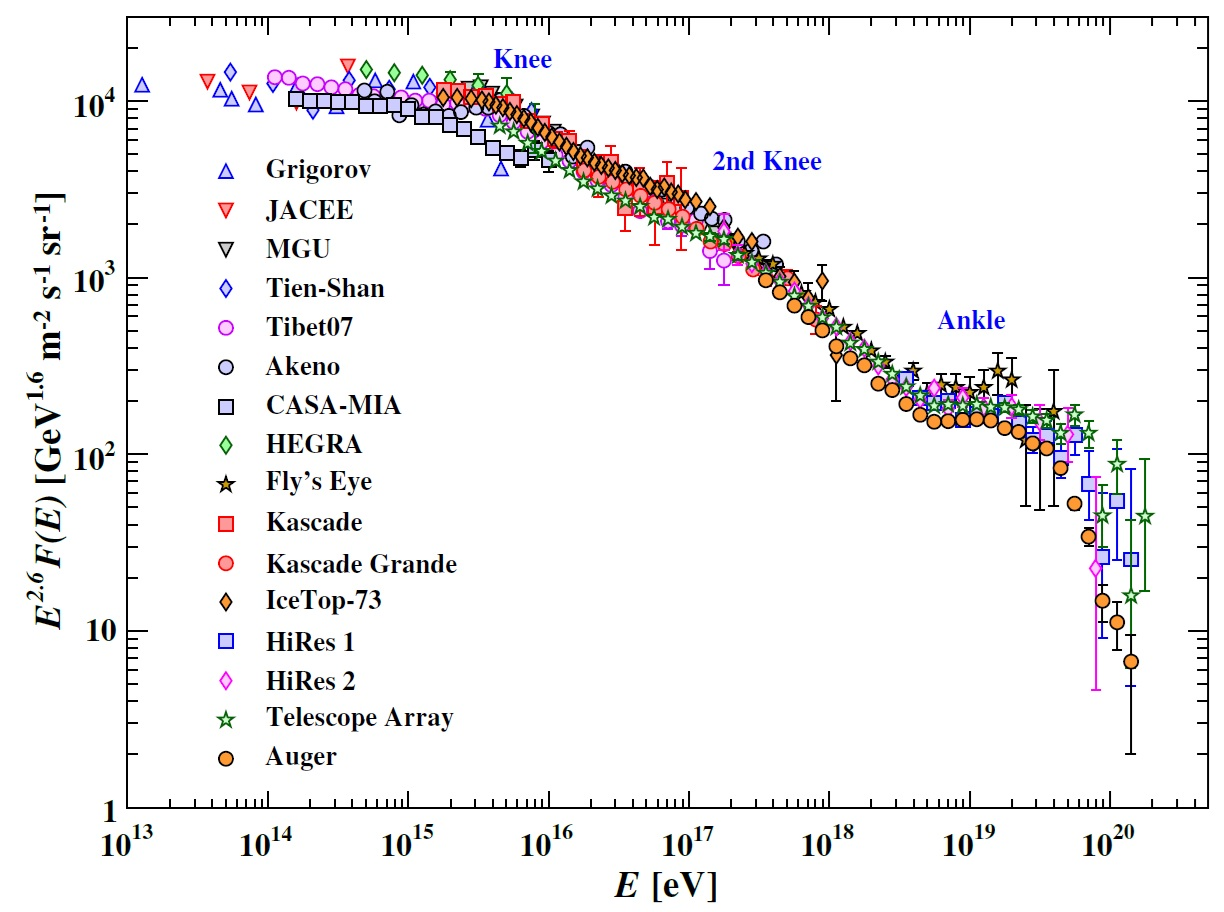
\includegraphics[width=\textwidth]{espectro_completo.jpg}
  \end{columns}
  \fuente{Fuente: PDG (2018).}
\end{frame}

\begin{frame}{Las estructuras del espectro a ultra-alta energía}
  \begin{columns}[c]
    \column{0.36\textwidth}
      \begin{itemize}
        \item \emph{Segunda rodilla} ($\sim10^{17}$~eV), \emph{tobillo}
          ($\sim5\times10^{18}$~eV), \emph{instep} ($\sim10^{19}$~eV) y
          \emph{supresión} ($>4\times10^{19}$~eV).
        \item Interpretar cada una (transición galáctica/extragaláctica,
          GZK, límite de las fuentes) requiere conocer \textbf{de qué está
          hecho} el primario.
      \end{itemize}
    \column{0.6\textwidth}
      \centering
      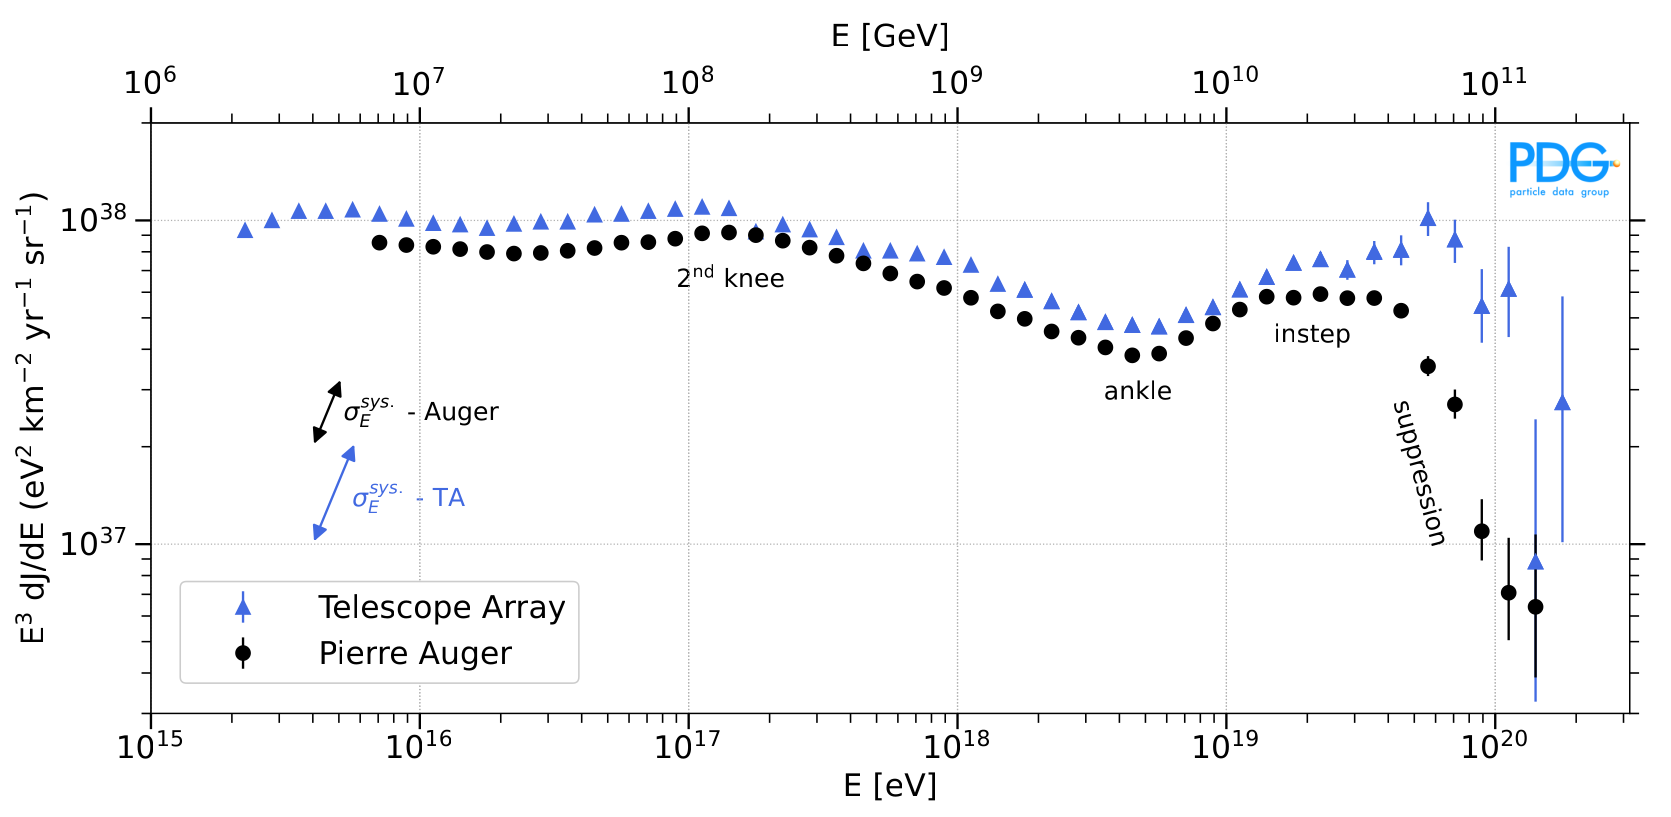
\includegraphics[width=\textwidth]{espectro_uhecr.png}
  \end{columns}
  \fuente{Fuente: PDG (2024).}
\end{frame}

\begin{frame}{Anatomía de una lluvia y el $X_{\max}$}
  \begin{columns}[T]
    \column{0.5\textwidth}
      \footnotesize
      \begin{itemize}
        \item Dos componentes: \textbf{electromagnética} ($e^\pm,\gamma$),
          numerosa, se absorbe rápido; \textbf{muónica}
          ($\pi^\pm,K^\pm\to\mu$), penetrante.
        \item Primero cada interacción \textbf{multiplica} las partículas;
          cuando su energía cae bajo un valor crítico dejan de
          multiplicarse y su número \textbf{disminuye}.
        \item $X_{\max}$: profundidad atmosférica (g/cm$^2$) con el
          \textbf{máximo número de partículas}. No es geométrico: la lluvia
          se sigue abriendo, lo que cae es el número.
        \item $\langle X_{\max}\rangle\propto\ln(E/A)$: más profundo a
          \textbf{mayor energía} y para \textbf{livianos}.
      \end{itemize}
    \column{0.48\textwidth}
      \centering
      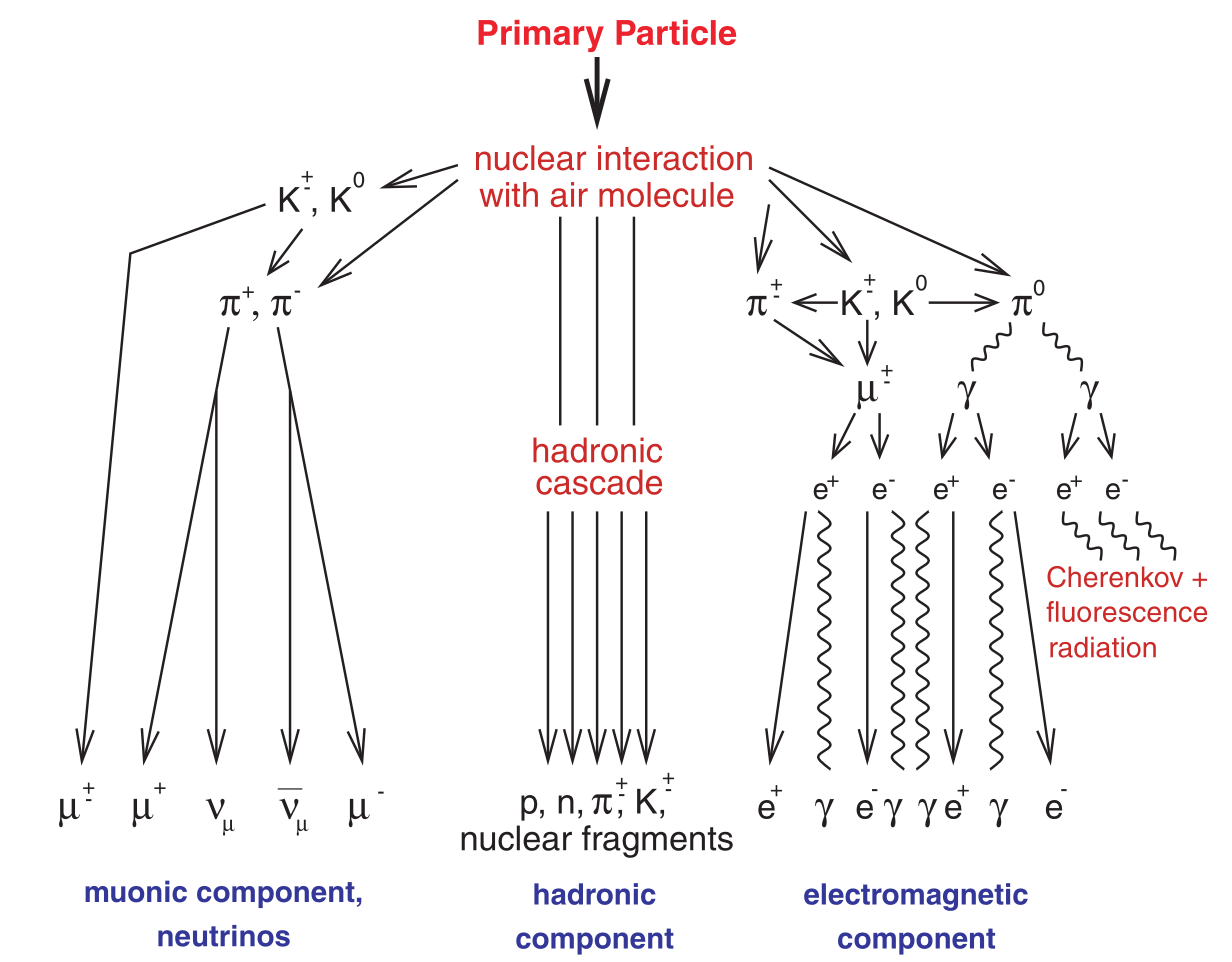
\includegraphics[width=\textwidth,height=4.5cm,keepaspectratio]{eas.png}

      \vspace{0.2em}
      \begin{tikzpicture}[x=1cm,y=1cm]
        \draw[-{Latex}] (0,0) -- (5.2,0) node[below left, font=\scriptsize] {$X$};
        \draw[-{Latex}] (0,0) -- (0,1.15) node[left, font=\scriptsize] {$N$};
        \draw[thick, itedaTeal, domain=0.05:5, samples=80, smooth]
          plot (\x, {1.0*pow(\x/1.8,1.8)*exp(1.8*(1-\x/1.8))});
        \draw[dashed, itedaOrange] (1.8,0) -- (1.8,1.0);
        \node[below, font=\scriptsize, itedaOrange] at (1.8,0) {$X_{\max}$};
        \node[font=\tiny] at (0.95,0.28) {multiplicación};
        \node[font=\tiny] at (3.3,0.28) {atenuación};
      \end{tikzpicture}
  \end{columns}
  \fuente{Fuente: Haungs \textit{et al.} (2003).}
\end{frame}

% ============================================================
\section{El Observatorio Pierre Auger}
% ============================================================

\begin{frame}{El Observatorio Pierre Auger}
  \begin{columns}[T]
    \column{0.5\textwidth}
      \begin{itemize}
        \item Malargüe, Mendoza. \textbf{3000~km$^2$}: el detector de rayos
          cósmicos más grande del mundo.
        \item \textbf{Detección híbrida}: 1660 tanques Cherenkov en agua (SD,
          espaciado 1500~m) + 24 telescopios de fluorescencia (FD) en 4 sitios.
        \item Arreglo \emph{Infill}: estaciones cada 750~m, umbral de energía
          más bajo.
        \item Duty cycle: SD $\sim$100\%; FD $\sim$15\% (sólo noches
          oscuras y despejadas).
      \end{itemize}
    \column{0.48\textwidth}
      \centering
      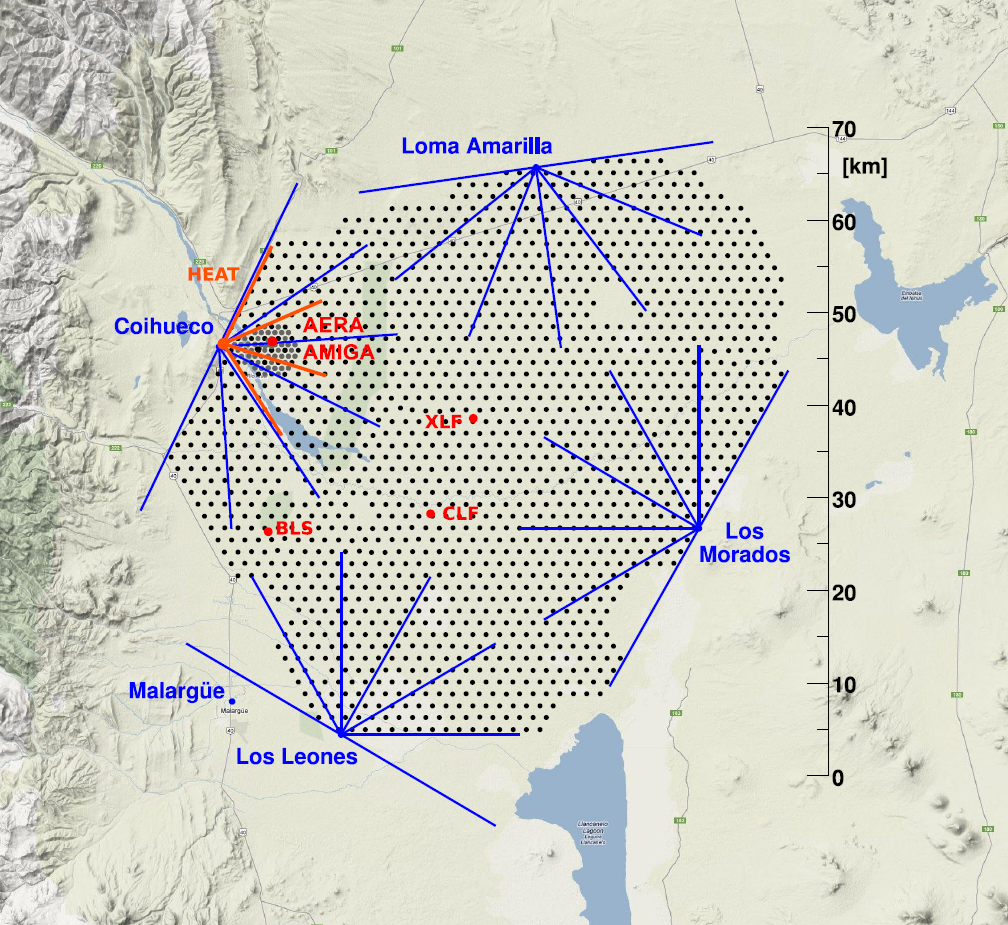
\includegraphics[width=\textwidth,height=5.3cm,keepaspectratio]{mapa_auger.png}
  \end{columns}
  \fuente{Fuente: Botti (2019).}
\end{frame}

\begin{frame}{AugerPrime}
  \begin{columns}[c]
    \column{0.44\textwidth}
      \begin{itemize}
        \item La gran actualización del Observatorio.
        \item Un \textbf{Centellador de Superficie} (SSD, $3.8$~m$^2$) sobre cada
          tanque: responde distinto a $e^\pm/\gamma$ que a muones.
        \item WCD+SSD permite \emph{desenredar estadísticamente} las dos
          componentes en superficie --- pero \textbf{no las separa
          físicamente}.
      \end{itemize}
    \column{0.5\textwidth}
      \centering
      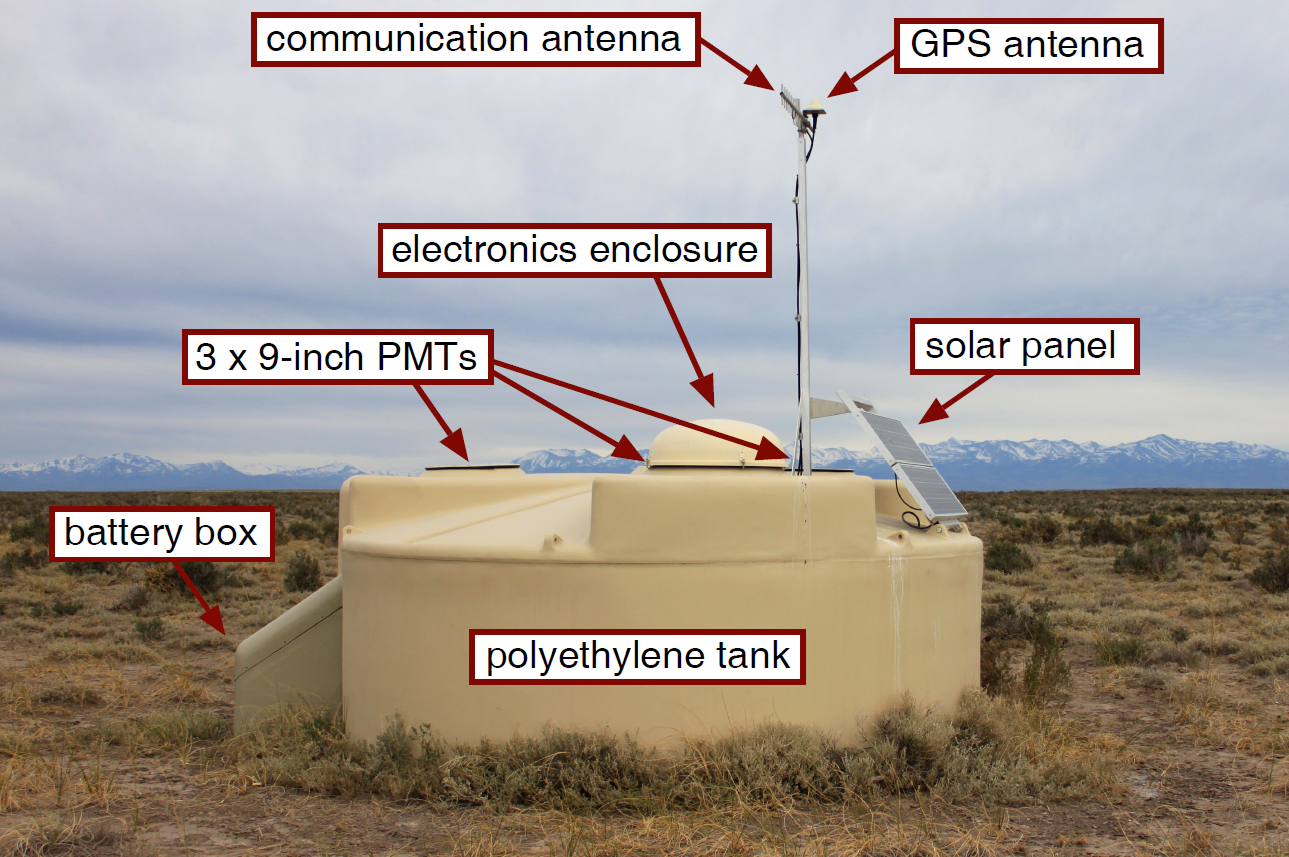
\includegraphics[width=\textwidth,height=5.1cm,keepaspectratio]{ssd.png}
  \end{columns}
  \fuente{Fuente: Botti (2019).}
\end{frame}

\begin{frame}{AMIGA y el Detector Subterráneo de Muones (UMD)}
  \begin{columns}[T]
    \column{0.48\textwidth}
      \begin{itemize}
        \item Centelladores \textbf{enterrados a 2.3~m} junto a cada tanque
          del \emph{Infill} $\Rightarrow \sim$\textbf{540~g/cm$^2$} de tierra,
          más de media atmósfera adicional.
        \item 3 módulos de 10~m$^2$ por estación, 64 tiras por módulo,
          lectura con fotomultiplicadores de silicio (SiPM).
        \item \textbf{Cuenta muones} directamente (modo de conteo
          segmentado).
      \end{itemize}
    \column{0.48\textwidth}
      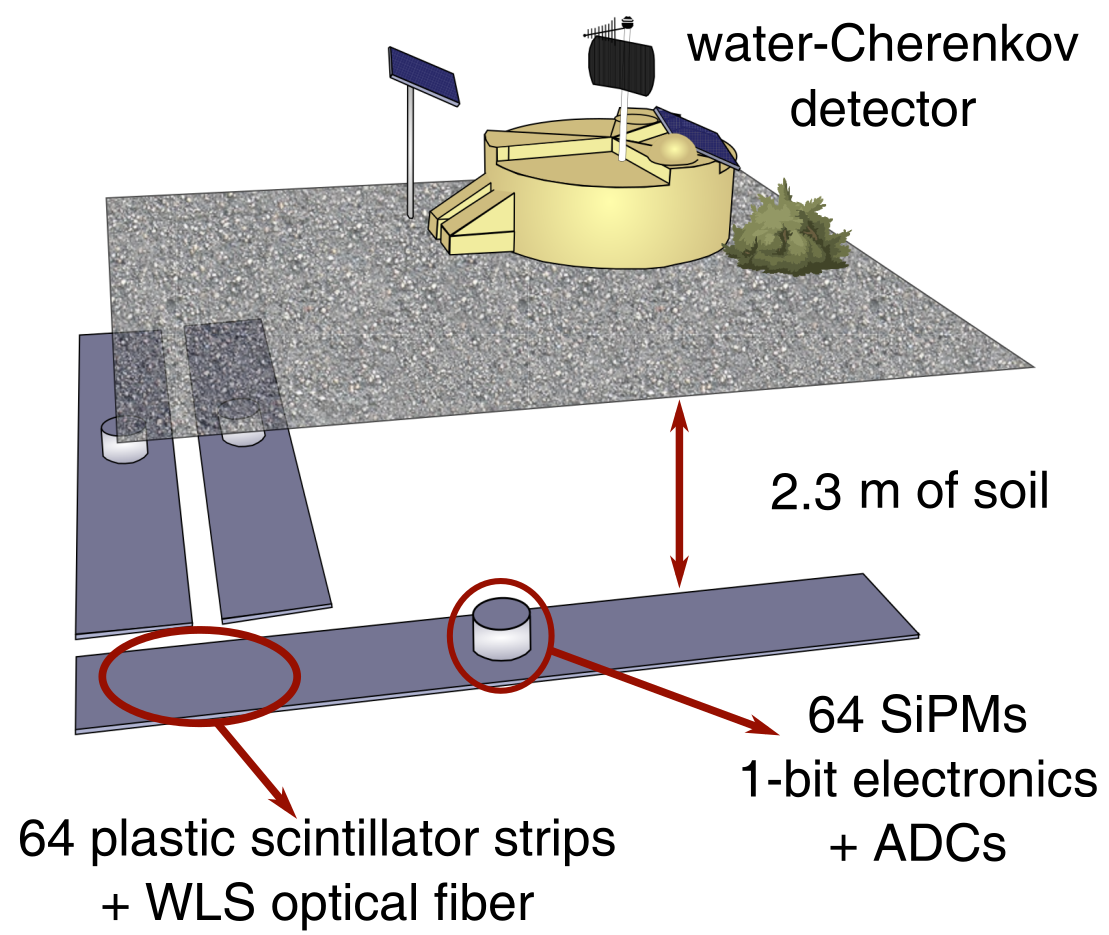
\includegraphics[width=\textwidth]{umd.png}
  \end{columns}
  \fuente{Fuente: Botti (2019).}
\end{frame}

\begin{frame}{¿Por qué el UMD es un detector distinto?}
  \begin{block}{El blindaje de tierra actúa como \textbf{doble filtro}}
    \begin{enumerate}
      \item \textbf{Absorción electromagnética}: la contribución de $e^\pm/\gamma$
        queda reducida a un nivel despreciable a las distancias al eje
        relevantes. La señal es \alert{muónica} --- sin la mezcla
        $S_{EM}+S_\mu$ del SD.
      \item \textbf{Umbral en energía}: sólo atraviesan la tierra los muones con
        $E_\mu \gtrsim 1~\text{GeV}/\cos\vartheta$, con $\vartheta$ el ángulo
        cenital \emph{local} de cada muón.
    \end{enumerate}
  \end{block}
  \vspace{0.4em}
  \begin{itemize}
    \item Los muones de la región tardía llegan más inclinados $\Rightarrow$
      atraviesan más tierra $\Rightarrow$ \textbf{umbral más alto}. Lo
      retomamos en la fenomenología.
  \end{itemize}
  \vspace{0.3em}
  \centering
  \large El UMD permite estudiar la física de la componente muónica aislada.
\end{frame}

% ============================================================
\section{Motivación y objetivos}
% ============================================================

\begin{frame}{Objetivos de la tesis}
  \small
  \begin{enumerate}
    \item \textbf{Asimetría azimutal en el UMD.} El estudio de la asimetría en
      el plano de la lluvia existe para el SD, pero no para el UMD, un detector
      nuevo. ¿Responde igual que el SD?
    \item \textbf{Sensibilidad a la masa del primario.} ¿Es la asimetría lo
      bastante distinta entre primarios como para distinguirlos?
    \item \textbf{Un modelo fenomenológico analítico.} Reunir todos los
      mecanismos que producen o modifican la asimetría, para hacer
      predicciones y contrastarlas con las simulaciones y los datos.
  \end{enumerate}
  \vspace{1.2em}
  \begin{block}{Herramientas}
    \textbf{Simulaciones} oficiales de la Colaboración (CORSIKA +
    \emph{Offline}), con diversos modelos hadrónicos y diversos primarios, en
    el \textbf{Anillo Denso} (12 estaciones virtuales a 450~m del eje) y en el
    arreglo \textbf{\emph{Infill}} real, más \textbf{datos de campo} del UMD
    en el arreglo \emph{Infill}.
  \end{block}
\end{frame}

\begin{frame}{Índice}
  \begin{enumerate}
    \setlength{\itemsep}{0.6em}
    \item Fenomenología de la asimetría azimutal y modelo analítico
    \item Asimetría en el UMD: simulaciones
    \item Comparación con el Detector de Superficie
    \item Origen de la diferencia entre SD y UMD
    \item Efectos de la reconstrucción
    \item Datos de campo y conclusiones
  \end{enumerate}
\end{frame}

% ============================================================
\section{Fenomenología de la asimetría azimutal}
% ============================================================

\begin{frame}{El plano de la lluvia}
  \begin{columns}[T]
    \column{0.44\textwidth}
      \begin{itemize}
        \item Coordenadas $(r,\phi)$ de cada estación, proyectada sobre el
          \textbf{plano perpendicular al eje}.
        \item Lluvia vertical: simetría circular.
        \item Lluvia inclinada:
        \begin{itemize}
          \item \textbf{Región temprana} ($\phi\approx0^\circ$): golpea el
            suelo primero, recorre \emph{menos} atmósfera.
          \item \textbf{Región tardía} ($\phi\approx\pm180^\circ$): golpea
            después, recorre \emph{más} atmósfera.
        \end{itemize}
        \item $\phi$ (de la estación) $\neq$ $\phi_{sh}$ (de arribo de la
          lluvia).
      \end{itemize}
    \column{0.54\textwidth}
      \centering
      \vspace{2.6em}
      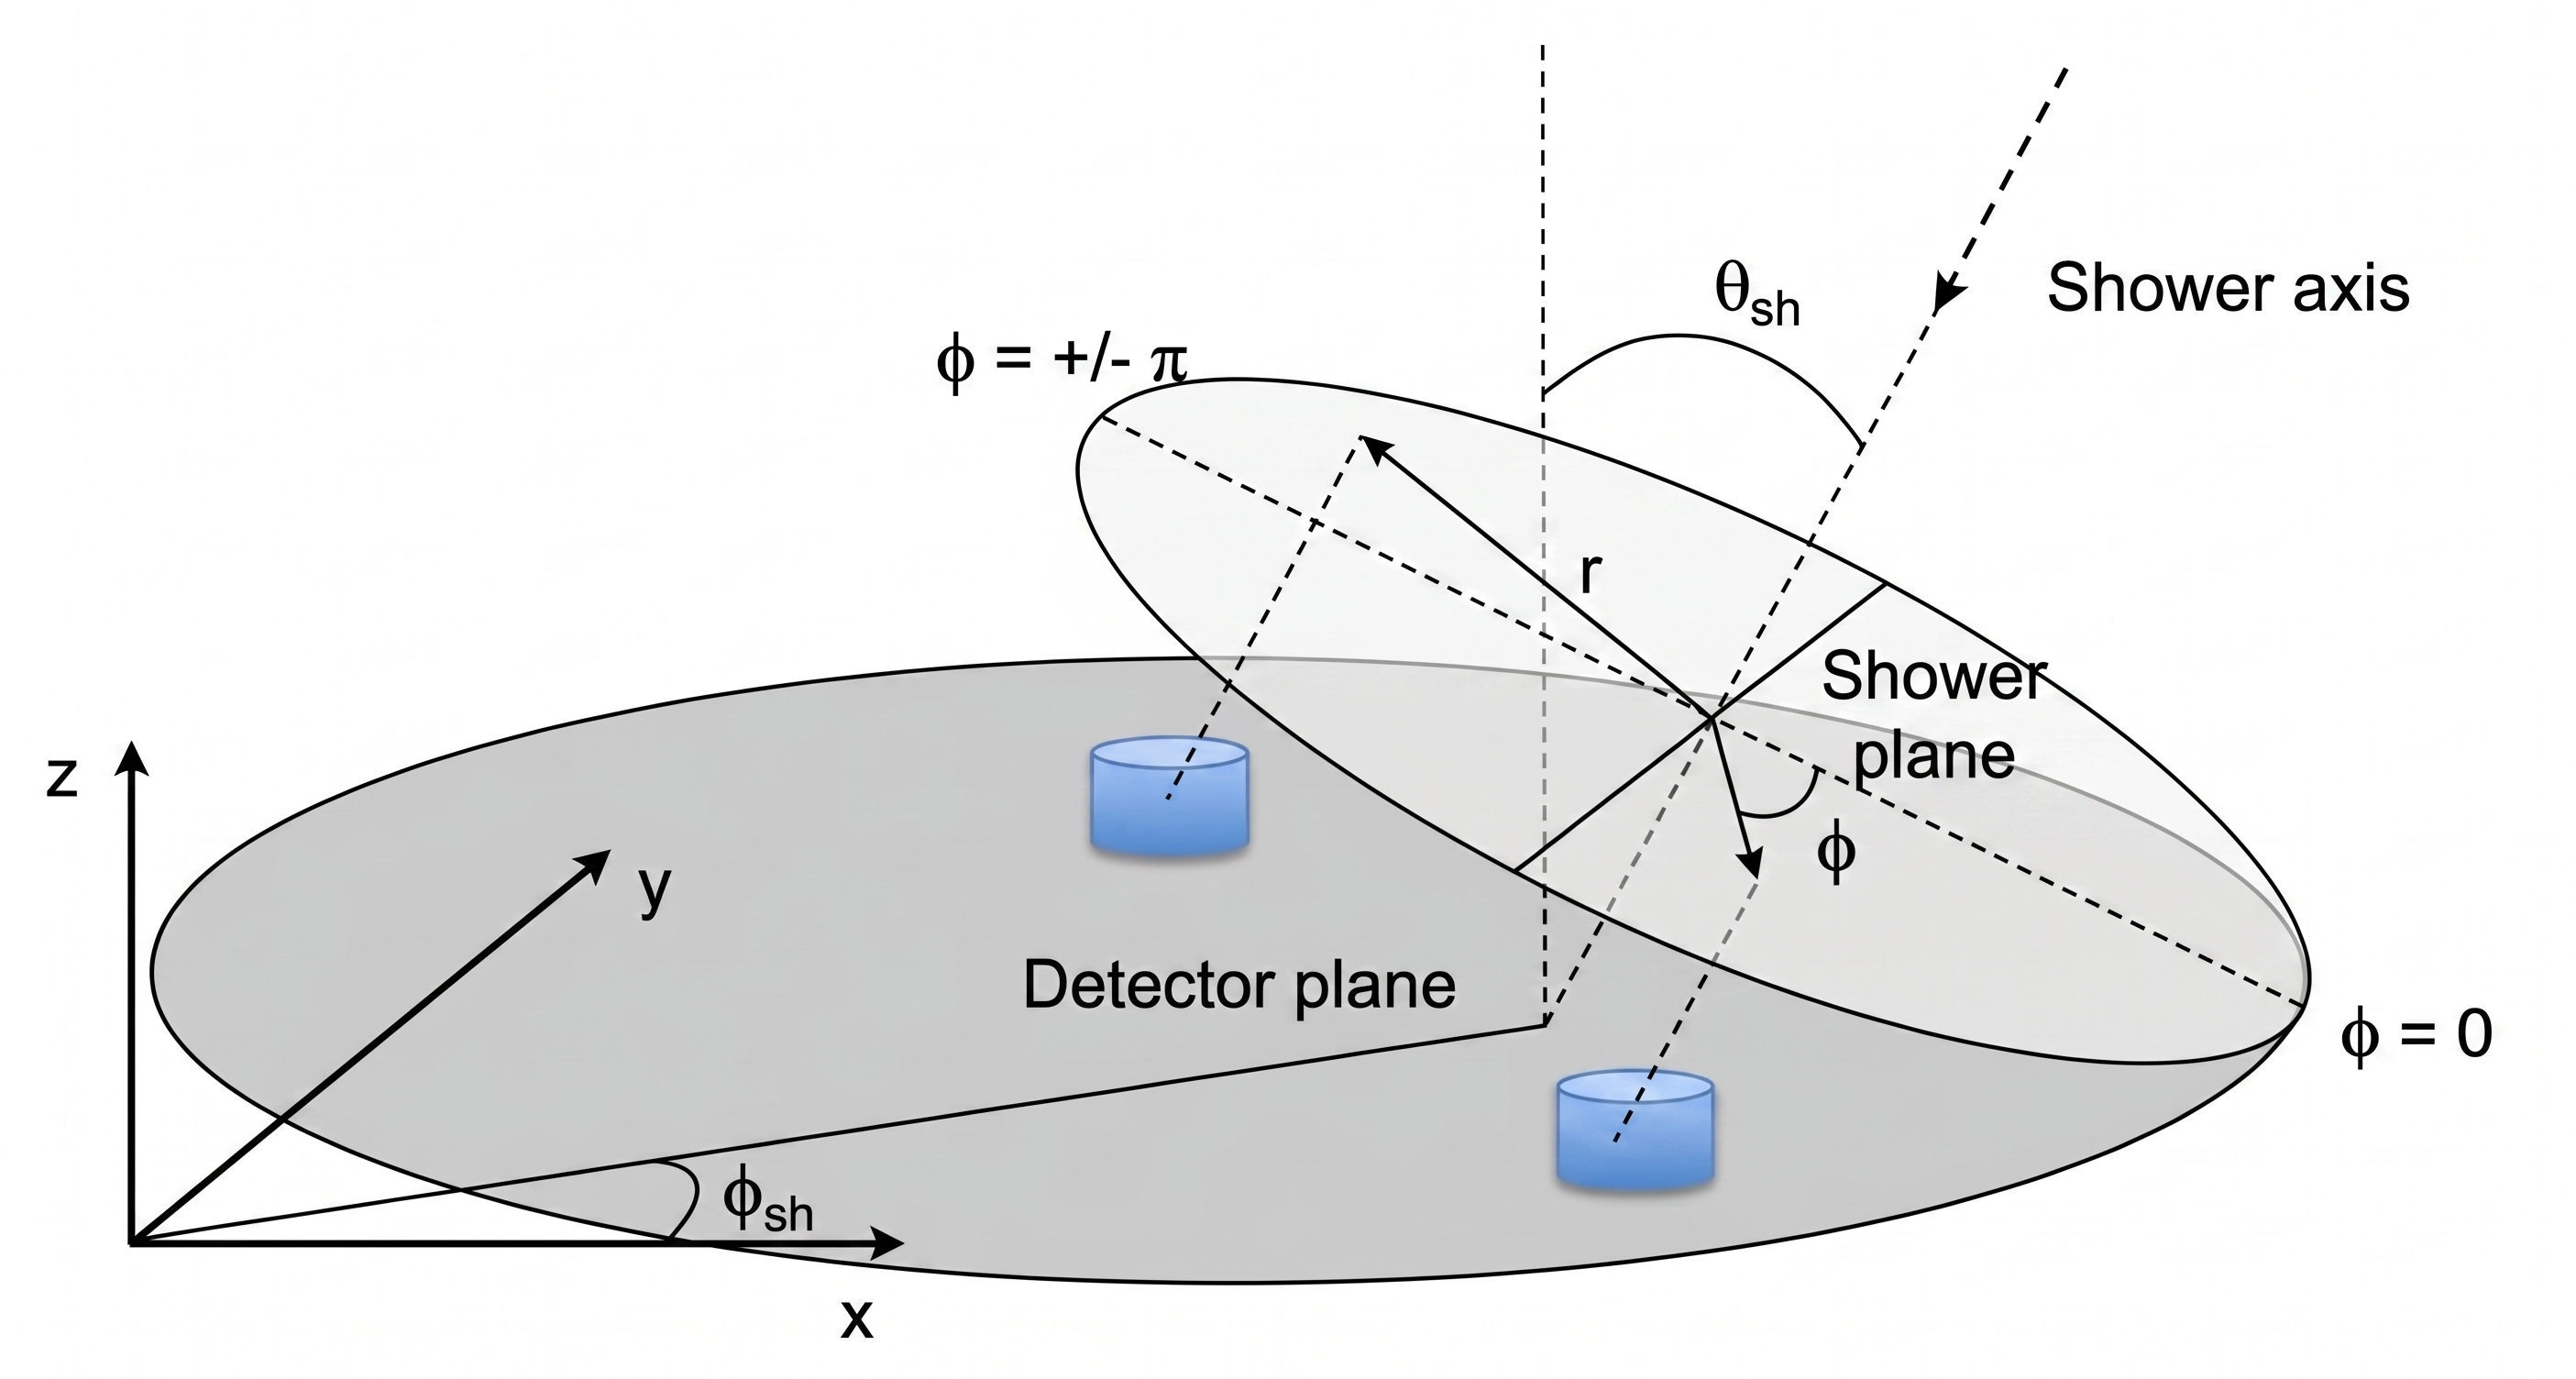
\includegraphics[width=\textwidth,height=5.0cm,keepaspectratio]{esquema_lluvia.jpeg}
  \end{columns}
\end{frame}

\begin{frame}{El observable: el primer armónico}
  \begin{equation*}
    S(r,\phi) = \langle S(r) \rangle \big(1 + A_1(r,\theta_{sh})\cos\phi\big)
  \end{equation*}
  \begin{itemize}
    \item $\langle S(r)\rangle$: densidad media a distancia $r$;
      $A_1$: amplitud de la modulación temprano-tardía.
    \item \textcolor{plotBlue}{$A_1>0$: exceso en la región temprana};
      \textcolor{plotMaroon}{$A_1<0$: exceso en la tardía}.
    \item Fase fijada en $\phi_0=0$, como en los estudios con el SD
      (Bradfield 2022).
    \item El signo de $A_1$ dice qué mecanismos dominan el balance, no
      identifica a uno solo.
  \end{itemize}
  \vspace{0.3em}
  \centering
  \alert{Para cada mecanismo: ¿qué es, cómo se modela y qué región favorece?}
\end{frame}

\begin{frame}{Mecanismo 1: atenuación}
  \begin{columns}[T]
    \column{0.55\textwidth}
      \small
      \begin{itemize}
        \item En cada tramo $\mathrm dL$ se pierde una fracción fija de las
          partículas que sobreviven:
          \begin{equation*}
            \frac{\mathrm dN}{\mathrm dL}=-\frac{N}{\lambda}
            \;\Rightarrow\;
            f_{att}(d)=e^{-d/\lambda}
          \end{equation*}
        \item Para muones: probabilidad de \textbf{no decaer en vuelo}
          \begin{equation*}
            \lambda_{dec}(p)=\frac{p}{m_\mu c}\,c\tau_\mu
            \simeq 6.2~\text{km}\times\frac{p}{1~\text{GeV}/c}
          \end{equation*}
        \item Como $\lambda_{dec}\propto p$, un muón de bajo momento decae en
          un recorrido más corto: el camino extra del lado tardío elimina
          una fracción mayor de muones blandos que de muones energéticos.
      \end{itemize}
    \column{0.42\textwidth}
      \begin{block}{Efecto}
        La región tardía recorre más camino:
        \begin{equation*}
          \frac{f_{att}(L_{\text{tardío}})}{f_{att}(L_{\text{temprano}})}
          = e^{-(L_{\text{tardío}}-L_{\text{temprano}})/\lambda} < 1
        \end{equation*}
        $\Rightarrow$ \favTemprana.
      \end{block}
      \small
      \begin{itemize}
        \item Actúa sobre ambas componentes, mucho más fuerte sobre la EM.
        \item En la práctica $\lambda$ es efectivo (incluye pérdidas de
          energía y umbrales): 5--10~km (Billoir) a 29--36~km (Armbruster).
      \end{itemize}
  \end{columns}
\end{frame}

\begin{frame}{Mecanismo 2: respuesta del detector}
  \begin{columns}[c]
    \column{0.57\textwidth}
      \small
      \begin{itemize}
        \item Bertou \& Billoir (2000): \textbf{lluvia estacionaria}, su
          distribución y la dirección de sus partículas no cambian a lo largo
          del eje.
        \item Las partículas no viajan paralelas al eje: se \textbf{abren}
          desde él un ángulo $\alpha$, con $\tan\alpha\simeq p_t/(-p_z)$.
        \item Abrirse hacia afuera las \textbf{inclina hacia la vertical} del
          lado temprano, $\vartheta=\theta_{sh}-\alpha$, y las
          \textbf{acuesta} del lado tardío, $\vartheta=\theta_{sh}+\alpha$.
        \item Un haz con $n$ partículas por unidad de área perpendicular, a un
          ángulo $\vartheta$ de la vertical, ve a una placa horizontal de área
          $A$ como: $A\cos\vartheta$ $\Rightarrow$ la atraviesan
          $N=nA\cos\vartheta$ partículas.
      \end{itemize}
    \column{0.41\textwidth}
      \centering
      \begin{tikzpicture}[x=0.62cm,y=0.62cm]
        % theta_sh = 50 grados; produccion en S = 4.2 * (sin 50, cos 50) = (3.22, 2.70).
        % Temprana: E = (3.22, 0), justo debajo de S (vartheta ~ 0).
        % Tardia: L = (-3.22, 0), a la misma distancia r = 2.07 del eje (vartheta ~ 67 grados).
        \draw[thick, itedaTealDark] (-3.9,0) -- (4.1,0);
        % plano de la lluvia y mismo r a ambos lados (marcas iguales)
        \draw[dotted, itedaGray] (-1.65,1.97) -- (1.65,-1.97);
        \node[font=\tiny, itedaGray, anchor=west] at (1.65,-1.97) {plano de la lluvia};
        \draw[very thick, itedaGray!60] (0,0) -- (1.33,-1.59);
        \draw[very thick, itedaGray!60] (0,0) -- (-1.33,1.59);
        \draw[itedaGray] (0.57,-0.87) -- (0.76,-0.72);
        \draw[itedaGray] (-0.76,0.72) -- (-0.57,0.87);
        \draw[dotted, itedaGray] (3.22,0) -- (1.33,-1.59);
        \draw[dotted, itedaGray] (-3.22,0) -- (-1.33,1.59);
        % eje
        \draw[dashed, itedaGray] (-0.6,-0.5) -- (3.22,2.70);
        \fill[itedaTealDark] (3.22,2.70) circle (2.5pt);
        \node[font=\tiny, above] at (3.22,2.75) {producción};
        \draw[dotted] (0,0) -- (0,1.5);
        \draw (0,0)++(40:0.75) arc (40:90:0.75);
        \node[font=\tiny] at ($(0,0)+(65:1.05)$) {$\theta_{sh}$};
        % trayectorias
        \draw[-{Latex[length=2mm]}, very thick, plotBlue] (3.22,2.70) -- (3.22,0.04);
        \draw[-{Latex[length=2mm]}, very thick, plotMaroon] (3.22,2.70) -- (-3.22,0.04);
        % angulos locales
        \node[font=\scriptsize, plotBlue, anchor=west] at (3.3,1.1) {$\vartheta\approx0$};
        \draw[dotted] (-3.22,0) -- (-3.22,1.7);
        \draw[plotMaroon] (-3.22,0)++(22.7:1.2) arc (22.7:90:1.2);
        \node[font=\scriptsize, plotMaroon] at ($(-3.22,0)+(58:1.5)$) {$\vartheta$};
        \node[font=\scriptsize, plotBlue, below] at (3.22,-0.05) {temprana};
        \node[font=\scriptsize, plotMaroon, below] at (-3.22,-0.05) {tardía};
      \end{tikzpicture}

      \vspace{0.5em}
      \raggedright
      \begin{block}{Bertou \& Billoir}
        \small
        $\mathcal{A}_{geo}=\big\langle p_t/(-p_z)\big\rangle\tan\theta_{sh}>0$:
        a primer orden en $\alpha$, el mismo resultado en otras variables.
        $\Rightarrow$ \favTemprana.
      \end{block}
  \end{columns}
\end{frame}

\begin{frame}{Mecanismo 2: placa, tanque y el umbral del UMD}
  \setbeamerfont{itemize/enumerate body}{size=\footnotesize}
  \begin{columns}[T]
    \column{0.55\textwidth}
      \footnotesize
      \begin{itemize}
        \item \textbf{Placa (UMD)}: cuenta los muones que la atraviesan; es
          el caso anterior.
        \item \textbf{Tanque, número de muones}: es un cuerpo 3D. La tapa
          (horizontal) atrapa más muones cuanto más verticales llegan: lado
          temprano. El costado (vertical) atrapa más cuanto más inclinados:
          lado tardío. Van en sentido contrario y \textbf{casi se compensan}.
        \item \textbf{Tanque, señal muónica}: cada muón deja luz según su
          recorrido en el agua. Donde entran más muones, recorren menos agua:
          \begin{equation*}
            \text{señal}\propto\underbrace{\mathcal{A}(\vartheta)}_{\text{muones}}
            \cdot\underbrace{\frac{V}{\mathcal{A}(\vartheta)}}_{\text{recorrido}}=V
          \end{equation*}
          \vspace{-1.1em}

          $\Rightarrow$ la señal \textbf{no se modula}.
      \end{itemize}
    \column{0.42\textwidth}
      \small
      \centering
      \renewcommand{\arraystretch}{1.1}
      \begin{tabular}{lc}
        \toprule
        Observable & $\kappa$\\
        \midrule
        Conteo en placa (\textbf{UMD}) & $1$\\
        Muones que entran al tanque & $\simeq0.3$\\
        Señal muónica del tanque (\textbf{SD}) & $0$\\
        \bottomrule
      \end{tabular}

      {\scriptsize $\kappa$: peso de la respuesta del detector en el modelo.}

      \vspace{0.3em}
      \raggedright
      \textbf{Umbral del UMD}: cada muón atraviesa
      $2.3~\text{m}/\cos\vartheta$ de tierra: el umbral es más alto del lado
      tardío, otro aporte positivo.
      \begin{block}{Efecto}
        \favTemprana, con magnitud distinta en UMD y SD.
      \end{block}
  \end{columns}
\end{frame}

\begin{frame}{Mecanismo 3: divergencia cinemática --- la producción}
  \begin{columns}[T]
    \column{0.52\textwidth}
      \small
      \begin{itemize}
        \item El mecanismo anterior trata a la lluvia como estacionaria. Acá
          los muones nacen a una distancia $D$ sobre el eje (Cazón
          \textit{et al.} 2012): los puntos temprano y tardío quedan a
          \textbf{distancias distintas} de la fuente.
        \item Con momento transversal $p_t$ salen a un ángulo
          $\sin\alpha=p_t/p\simeq c\,p_t/E$.
        \item Distribución de $p_t$:\;
          $\mathrm dN/\mathrm dp_t\propto p_t\,e^{-p_t/Q}$.
        \item La densidad cae con la distancia recorrida:
          \begin{equation*}
            S(d,\alpha)\propto\frac{1}{d^2}\,\frac{\mathrm dN}{\mathrm d\Omega}(\alpha)
          \end{equation*}
      \end{itemize}
    \column{0.45\textwidth}
      \centering
      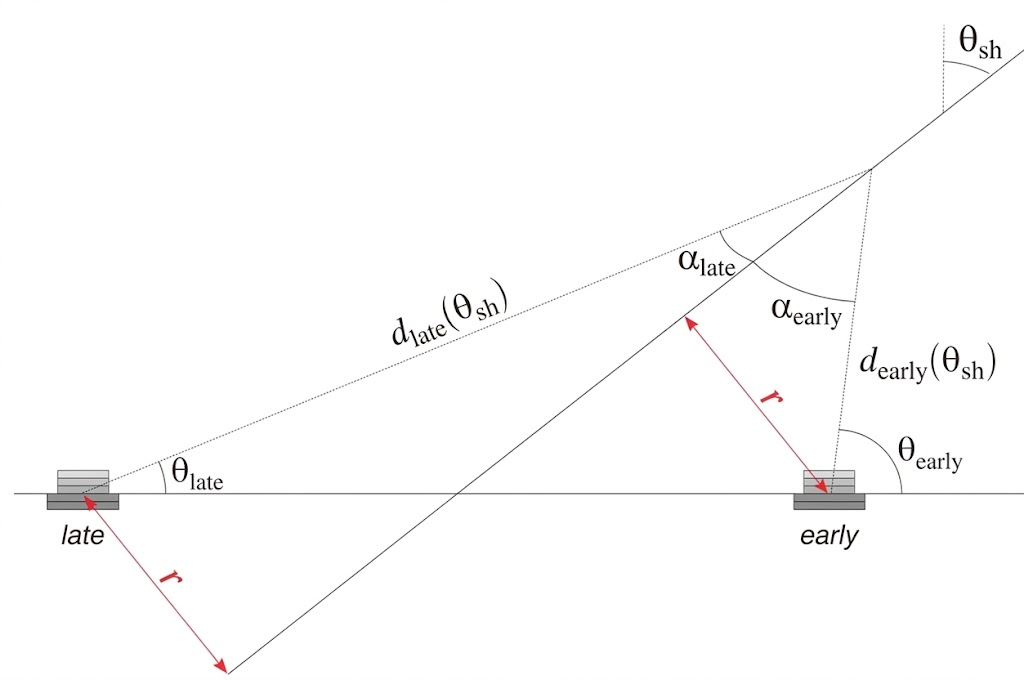
\includegraphics[width=\textwidth,height=4.0cm,keepaspectratio]{efecto_geo_luce_icrc2021.png}

      \small Para llegar al mismo $r$, la región tardía está \textbf{más lejos}
      ($d_{\text{tardío}}>d_{\text{temprano}}$) y requiere un ángulo
      \textbf{menor} ($\alpha_{\text{tardío}}<\alpha_{\text{temprano}}$).
  \end{columns}
  \fuente{Adaptada de Luce \textit{et al.}, ICRC 2021.}
\end{frame}

\begin{frame}{Divergencia cinemática: del momento al ángulo}
  \begin{itemize}
    \item A momento $p$ fijo:\quad
      $\mathrm d\Omega\propto\sin\alpha\,\mathrm d\alpha$,\qquad
      $\mathrm dp_t=p\cos\alpha\,\mathrm d\alpha$
      \quad$\Rightarrow$\quad
      $\mathrm d\Omega\propto\dfrac{p_t}{p^2\cos\alpha}\,\mathrm dp_t$
    \item Regla de la cadena --- el factor lineal $p_t$ se cancela:
  \end{itemize}
  \begin{equation*}
    \frac{\mathrm dN}{\mathrm d\Omega}
    =\frac{\mathrm dN}{\mathrm dp_t}\,\frac{\mathrm dp_t}{\mathrm d\Omega}
    \propto\Big(\cancel{p_t}\,e^{-p_t/Q}\Big)\Big(\frac{p^2\cos\alpha}{\cancel{p_t}}\Big)
    =p^2\cos\alpha\;e^{-p_t/Q}
  \end{equation*}
  \begin{itemize}
    \item Reemplazando $p_t=p\sin\alpha\simeq E\sin\alpha/c$ y agregando la
      dilución espacial $1/d^2$, para muones de una misma energía:
  \end{itemize}
  \begin{equation*}
    \boxed{\;S(d,\alpha)\propto\frac{1}{d^2}\,\cos\alpha\,
    \exp\!\left(-\frac{E\sin\alpha}{cQ}\right)\;}
  \end{equation*}
\end{frame}

\begin{frame}{Divergencia cinemática: ¿temprana o tardía?}
  \begin{equation*}
    \frac{S_{\text{tardío}}}{S_{\text{temprano}}} \approx
    \underbrace{\left(\frac{d_{\text{temprano}}}{d_{\text{tardío}}}\right)^{\!2}}_{\text{dilución}\,<\,1}
    \cdot
    \underbrace{\frac{\cos\alpha_{\text{tardío}}}{\cos\alpha_{\text{temprano}}}}_{\text{esp.\ de fases}\,>\,1}
    \cdot
    \underbrace{\exp\!\left(\frac{(\sin\alpha_{\text{temprano}}-\sin\alpha_{\text{tardío}})\,E}{cQ}\right)}_{\text{ganancia cinemática}\,>\,1}
  \end{equation*}
  \begin{columns}[T]
    \column{0.46\textwidth}
      \small
      \begin{itemize}
        \item La \textbf{dilución} \favTemprana.
        \item La \textbf{emisión angular} (2.º y 3.º factor) \favTardia: los
          muones salen preferentemente cerca del eje.
        \item El signo lo decide la \textbf{energía del muón}, a través del
          tercer factor.
      \end{itemize}
    \column{0.51\textwidth}
      \footnotesize
      \begin{block}{¿Y con muones de todas las energías?}
        Un detector \textbf{suma} muones de todas las energías, y los
        energéticos salen en un cono angosto: concentran densidad donde
        llegan.\\[0.4em]
        $\Rightarrow$ Un modelo tiene que tener en cuenta el \textbf{espectro
        real de momentos} de los muones.
      \end{block}
  \end{columns}
\end{frame}

\begin{frame}{Mecanismo 4: campo geomagnético}
  \begin{itemize}
    \item La fuerza de Lorentz $\vec F=q\,\vec v\times\vec B$ separa
      lateralmente $\mu^+$ y $\mu^-$.
    \item La deformación es aproximadamente \textbf{elíptica} y su orientación
      depende de la dirección de arribo respecto de $\vec B$: su proyección
      sobre $\cos\phi$ es pequeña.
    \item Al promediar lluvias con distintas direcciones, agrega
      \textbf{dispersión} al perfil azimutal, no un signo definido.
    \item Domina sólo en lluvias muy inclinadas ($\theta_{sh}\gtrsim70^\circ$).
  \end{itemize}
  \begin{block}{En esta tesis}
    Efecto de segundo orden para $\theta_{sh}\le65^\circ$: no se incluye en el
    modelo.
  \end{block}
\end{frame}

\begin{frame}{Un modelo de juguete para el signo de $A_1$}
  \small
  Una fuente puntual de muones sobre el eje, a distancia $D$ del núcleo, con
  propagación rectilínea. Para muones de momento $p$:
  \begin{equation*}
    S(r,\phi\,|\,p) \propto
    \underbrace{\frac{1}{d^2}\,f(\alpha\,|\,p)}_{\text{divergencia}}\;
    \underbrace{e^{-d/\lambda(p)}}_{\text{atenuación}}\;
    \underbrace{\mathcal{R}(\vartheta)}_{\text{respuesta}}\;
    \underbrace{\Theta_{\mathrm{UMD}}}_{\text{umbral}}
  \end{equation*}
  \begin{itemize}
    \item \textbf{Distancia de la fuente a la estación}, la $d$ de los
      términos de divergencia y atenuación:
      \quad $d(\phi)=\sqrt{(D-r\tan\theta_{sh}\cos\phi)^2+r^2}$
    \item \textbf{Ángulos} de cada factor: el de emisión,
      $\sin\alpha=r/d$, entra en $f$; el cenital local,
      $\cos\vartheta=D\cos\theta_{sh}/d$, entra en la respuesta y en el umbral.
    \item \textbf{Umbral} (sólo UMD): un muón llega al centellador si su
      momento alcanza para atravesar la tierra a lo largo de su trayectoria,
      $p>p_{\mathrm{UMD}}/\cos\vartheta$, con $p_{\mathrm{UMD}}\approx1$~GeV/$c$
      en incidencia vertical. Es más alto del lado tardío. En el SD,
      $\Theta=1$.
  \end{itemize}
\end{frame}

\begin{frame}{Del muón a la población}
  \begin{columns}[c]
    \column{0.55\textwidth}
      \begin{itemize}
        \item Un detector no ve muones de un único momento: \textbf{suma todos
          los que llegan}.
        \item El espectro de producción cae como una \textbf{ley de potencias
          inversa}:
          \begin{equation*}
            G(p)\propto p^{-\gamma},\qquad \gamma\approx2.6
          \end{equation*}
          muchos muones blandos, pocos energéticos.
        \item Cada región suma \emph{su} población antes de comparar:
          \begin{equation*}
            S(r,\phi)\propto\int G(p)\,S(r,\phi\,|\,p)\,\mathrm dp
          \end{equation*}
      \end{itemize}
    \column{0.42\textwidth}
      \begin{block}{¿Cómo se obtiene $A_1$?}
        \small
        Como $S\propto1+A_1\cos\phi$:
        \begin{itemize}
          \item temprana ($\phi=0$): $\langle S\rangle(1+A_1)$
          \item tardía ($\phi=\pi$): $\langle S\rangle(1-A_1)$
        \end{itemize}
        Despejando:
        \begin{equation*}
          A_1=\frac{S_{\text{temp}}-S_{\text{tard}}}{S_{\text{temp}}+S_{\text{tard}}}
        \end{equation*}
      \end{block}
  \end{columns}
\end{frame}

\begin{frame}{Linealización: un término por mecanismo}
  A primer orden en $r/D$:
  \begin{equation*}
    A_1 \simeq \Big[\,\underbrace{2}_{\text{dilución}} \;-\; \underbrace{s}_{\text{emisión angular}} \;+\; \underbrace{D/\lambda}_{\text{atenuación}} \;+\; \underbrace{\kappa}_{\text{respuesta}}\,\Big]\,\frac{r}{D}\,\tan\theta_{sh}
  \end{equation*}
  \begin{columns}[T]
    \column{0.52\textwidth}
      \small
      \begin{itemize}
        \item \textbf{2}: la región temprana está más cerca de la fuente.
        \item $\mathbf{D/\lambda}$: el camino hasta la tardía es más largo.
        \item $\boldsymbol{\kappa}$: respuesta del detector (1 en el UMD, 0
          para la señal del SD).
        \item $\mathbf{s\simeq p\,r/(Q\,D)}$: emisión angular. Es el
          \textbf{único término negativo} y crece con el momento del muón.
      \end{itemize}
    \column{0.45\textwidth}
      \begin{block}{Caso particular: Armbruster (2018)}
        \small
        Señal del SD ($\kappa=0$), distribución angular $f\propto\alpha^{-\gamma_{\mathrm{ADF}}}$:
        \begin{equation*}
          A_1=\big(2-\gamma_{\mathrm{ADF}}+D/\lambda\big)\frac{r}{D}\tan\theta_{sh}
        \end{equation*}
        retomada por Luce \textit{et al.} (ICRC 2021).
      \end{block}
  \end{columns}
\end{frame}

\begin{frame}{¿Qué signo tiene la población?}
  \begin{columns}[T]
    \column{0.55\textwidth}
      \small
      \begin{enumerate}
        \item \textbf{Un solo muón} da $A_1<0$ sólo si $s>2$ (sin atenuación ni
          respuesta), es decir si su momento supera el \textbf{momento de cruce}
          \begin{equation*}
            p^*\simeq\frac{2\,Q\,D}{r}\quad(\approx1.9~\text{GeV}/c\text{ a }r=1200~\text{m})
          \end{equation*}
          Con atenuación y respuesta, el cruce sube todavía más.
        \item \textbf{¿Qué momento tienen los muones que llegan a $r$?} Para
          llegar necesitan $p_t\simeq p\,r/D$, y Cazón suprime los $p_t$
          grandes como $e^{-p_t/Q}=e^{-p/p_0}$, con $p_0=QD/r$.
        \item Como $p_0=p^*/2$, los muones que llegan están \textbf{por debajo
          del cruce}: la población da $A_1>0$.
      \end{enumerate}
    \column{0.42\textwidth}
      \centering
      \begin{tikzpicture}[x=1cm,y=1cm]
        \fill[plotMaroon!12] (3.0,0) rectangle (4.9,2.0);
        \draw[-{Latex}] (0,0) -- (5.0,0) node[below left, font=\scriptsize] {$p$};
        \draw[-{Latex}] (0,0) -- (0,2.1);
        \draw[thick, itedaTeal, domain=0:4.8, samples=60, smooth]
          plot (\x, {1.8*exp(-\x/1.5)});
        \draw[dashed, itedaTealDark] (1.5,0) -- (1.5,1.2);
        \node[below, font=\scriptsize] at (1.5,0) {$p_0$};
        \draw[dashed, plotMaroon] (3.0,0) -- (3.0,1.2);
        \node[below, font=\scriptsize, plotMaroon] at (3.0,0) {$p^*=2p_0$};
        \node[font=\scriptsize, plotMaroon, align=center] at (3.95,0.8) {$A_1<0$};
        \node[font=\scriptsize, plotBlue, align=center] at (0.8,0.55) {$A_1>0$};
        \node[font=\tiny, itedaTeal, anchor=west] at (0.75,1.55) {muones que llegan a $r$};
      \end{tikzpicture}

      \vspace{0.4em}
      {\footnotesize Los muones que favorecerían a la región tardía son
      justamente los que casi no llegan lejos del eje.}
  \end{columns}
\end{frame}

\begin{frame}{Resultados del modelo: la predicción}
  \centering
  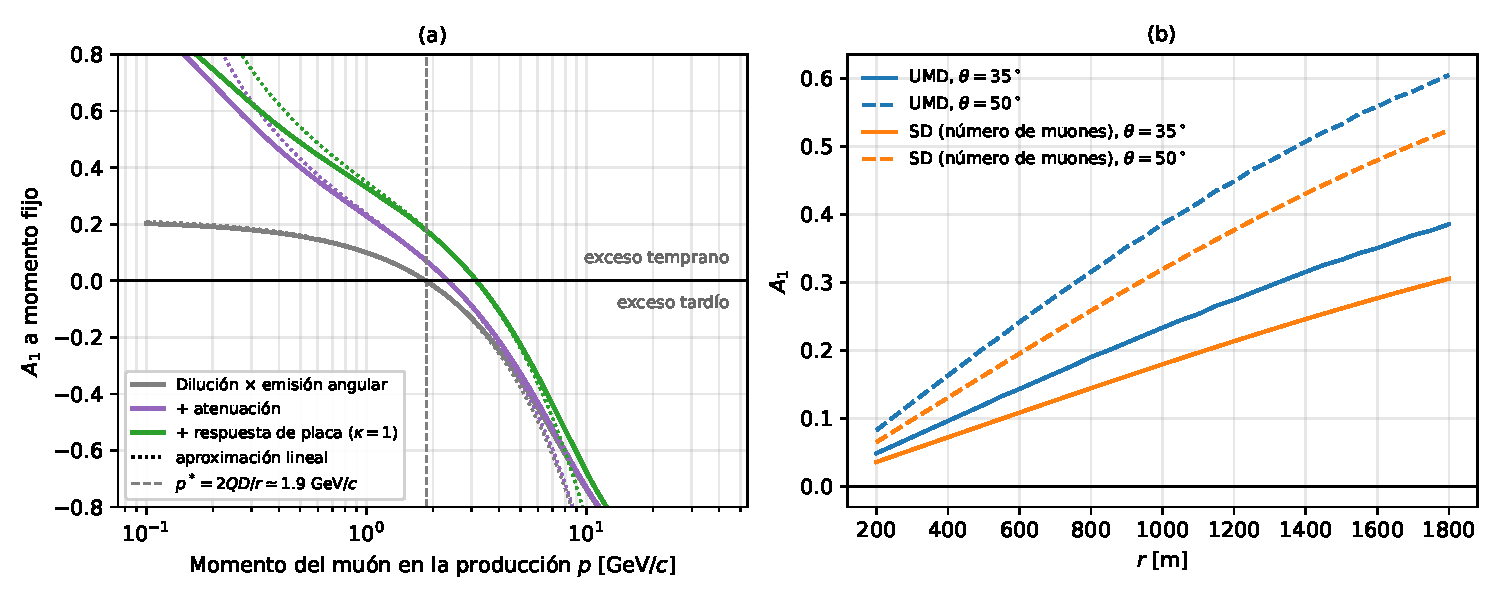
\includegraphics[width=0.92\textwidth,height=3.25cm,keepaspectratio]{modelo_juguete.pdf}
  \begin{columns}[T]
    \column{0.48\textwidth}
      \footnotesize
      \textbf{(a) Un solo momento} ($r=1200$~m, $\theta_{sh}=35^\circ$):
      $A_1<0$ sólo por encima de $p^*$. La atenuación y la respuesta de placa
      corren el cruce de 1.9 a 2.3 y a 3.2~GeV/$c$.
    \column{0.48\textwidth}
      \footnotesize
      \textbf{(b) Población:} positiva a todo $r$, crece con $r$ y $\theta_{sh}$,
      y $A_1^{\mathrm{UMD}}>A_1^{\mathrm{SD}}$.
  \end{columns}
  \vspace{0.2em}
  \begin{alertblock}{Predicción}
    \footnotesize $A_1>0$ en el UMD y en el SD, creciente con $r$ y con
    $\theta_{sh}$. El signo se mantiene al variar $D$, $Q$ y $\gamma$.
  \end{alertblock}
\end{frame}

% ============================================================
\section{El UMD en simulaciones}
% ============================================================


\begin{frame}{Anillo Denso: un ejemplo de ajuste}
  \badgeAD
  \begin{columns}[c]
    \column{0.58\textwidth}
      \centering
      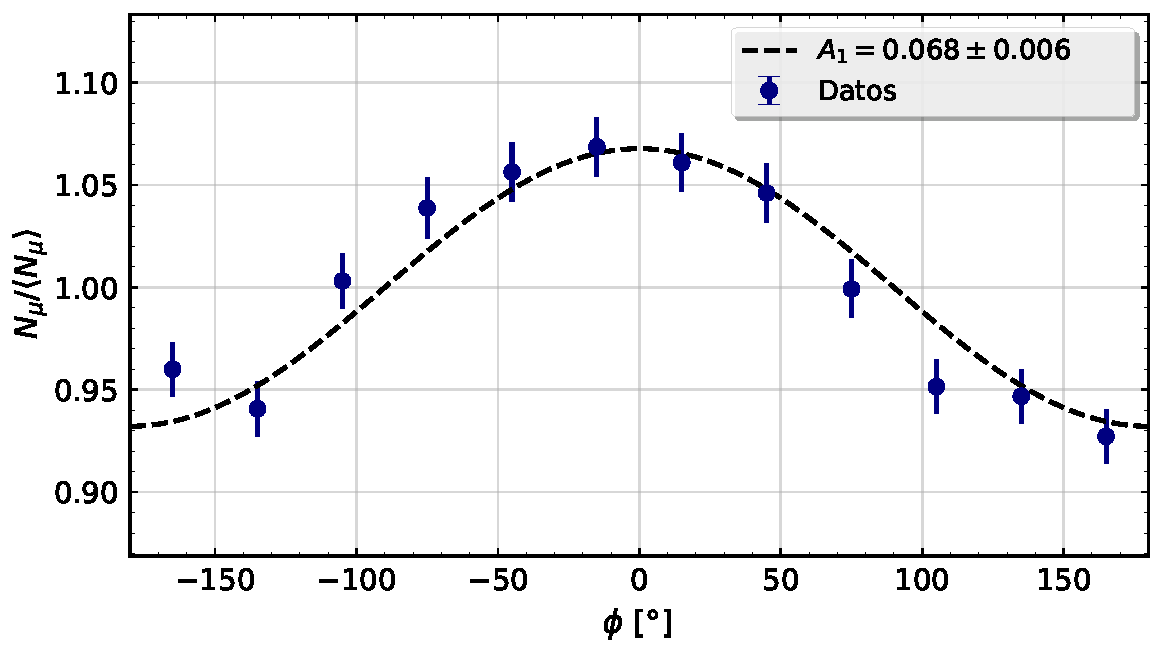
\includegraphics[width=\textwidth,height=5.4cm,keepaspectratio]{Ajuste_UMD_REC_Bin9.pdf}
    \column{0.39\textwidth}
      \begin{itemize}
        \item Protones, $59.3^\circ<\theta_{sh}<65^\circ$, muones reconstruidos
          por el UMD.
        \item Modulación clara: \alert{$\approx14\%$ pico a pico}
          ($\pm7\%$ respecto de la media).
        \item Máximo en la región temprana: \textbf{$A_1>0$, como predice el
          modelo}.
        \item $\chi^2_\nu\approx1$.
      \end{itemize}
  \end{columns}
\end{frame}

\begin{frame}{$A_1$ vs.\ $\theta$: UMD y SD}
  \badgeAD
  \begin{columns}[c]
    \column{0.58\textwidth}
      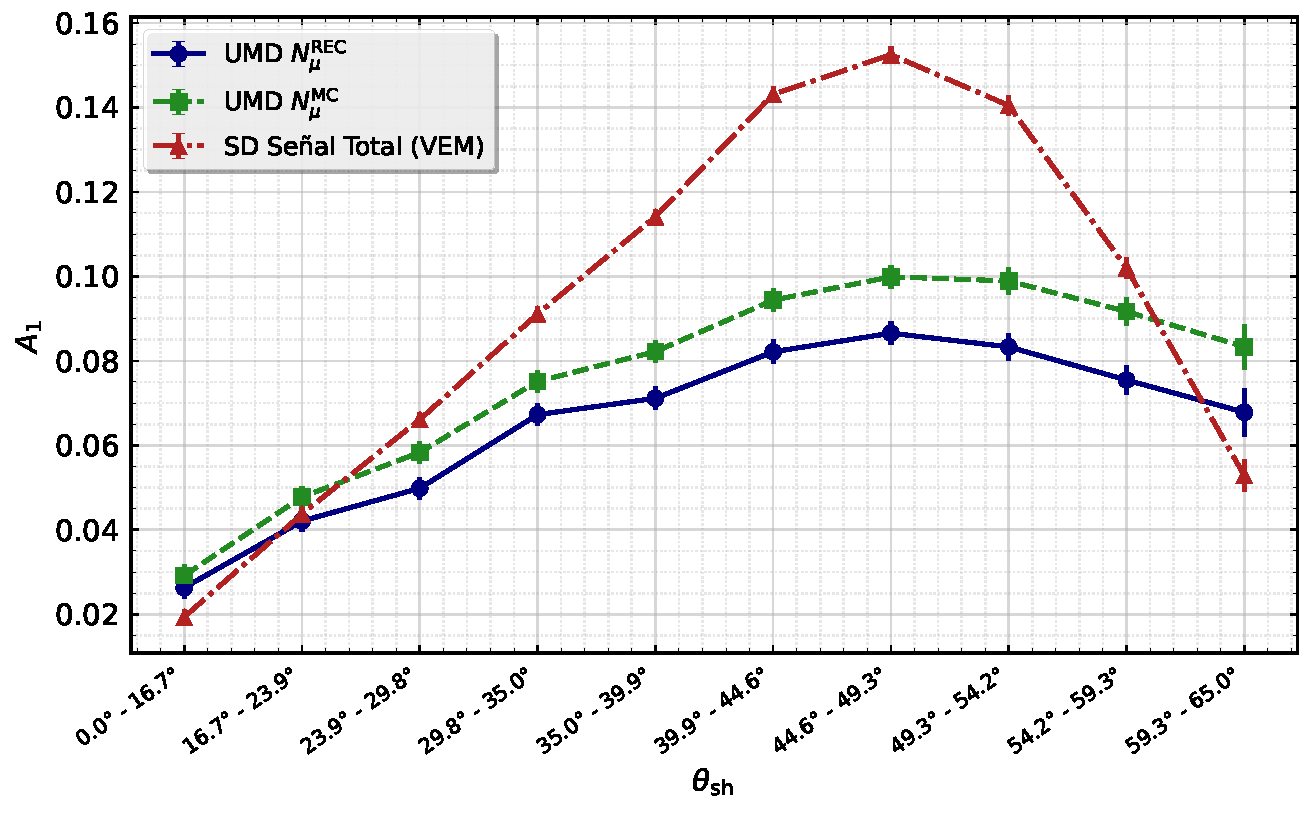
\includegraphics[width=\textwidth]{Evolucion_Asimetria_vs_Theta.pdf}
    \column{0.39\textwidth}
      \small
      \begin{itemize}
        \item $\theta$ bajo: el SD, dominado por la EM, tiene $A_1$ mucho
          mayor.
        \item $\theta\gtrsim50^\circ$: la EM se absorbe y el SD queda
          \textbf{por debajo} del UMD.
        \item El UMD crece con $\theta$.
        \item \alert{Notar}: UMD REC $<$ UMD MC. Volvemos a esto más adelante.
      \end{itemize}
  \end{columns}
\end{frame}

\begin{frame}{Robustez del observable}
  \badgeAD
  \begin{columns}[T]
    \column{0.49\textwidth}
      \centering
      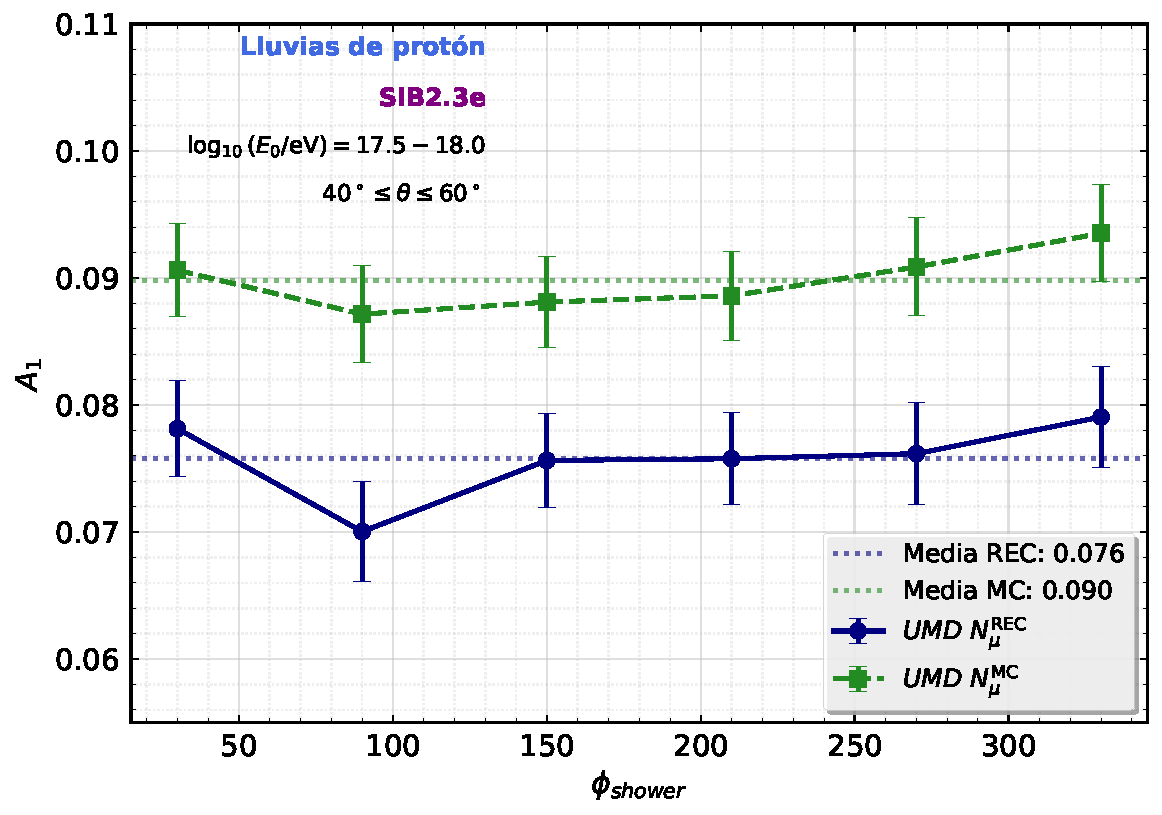
\includegraphics[width=\textwidth,height=4.3cm,keepaspectratio]{DenseRing_Systematics_Isotropy.pdf}
    \column{0.49\textwidth}
      \centering
      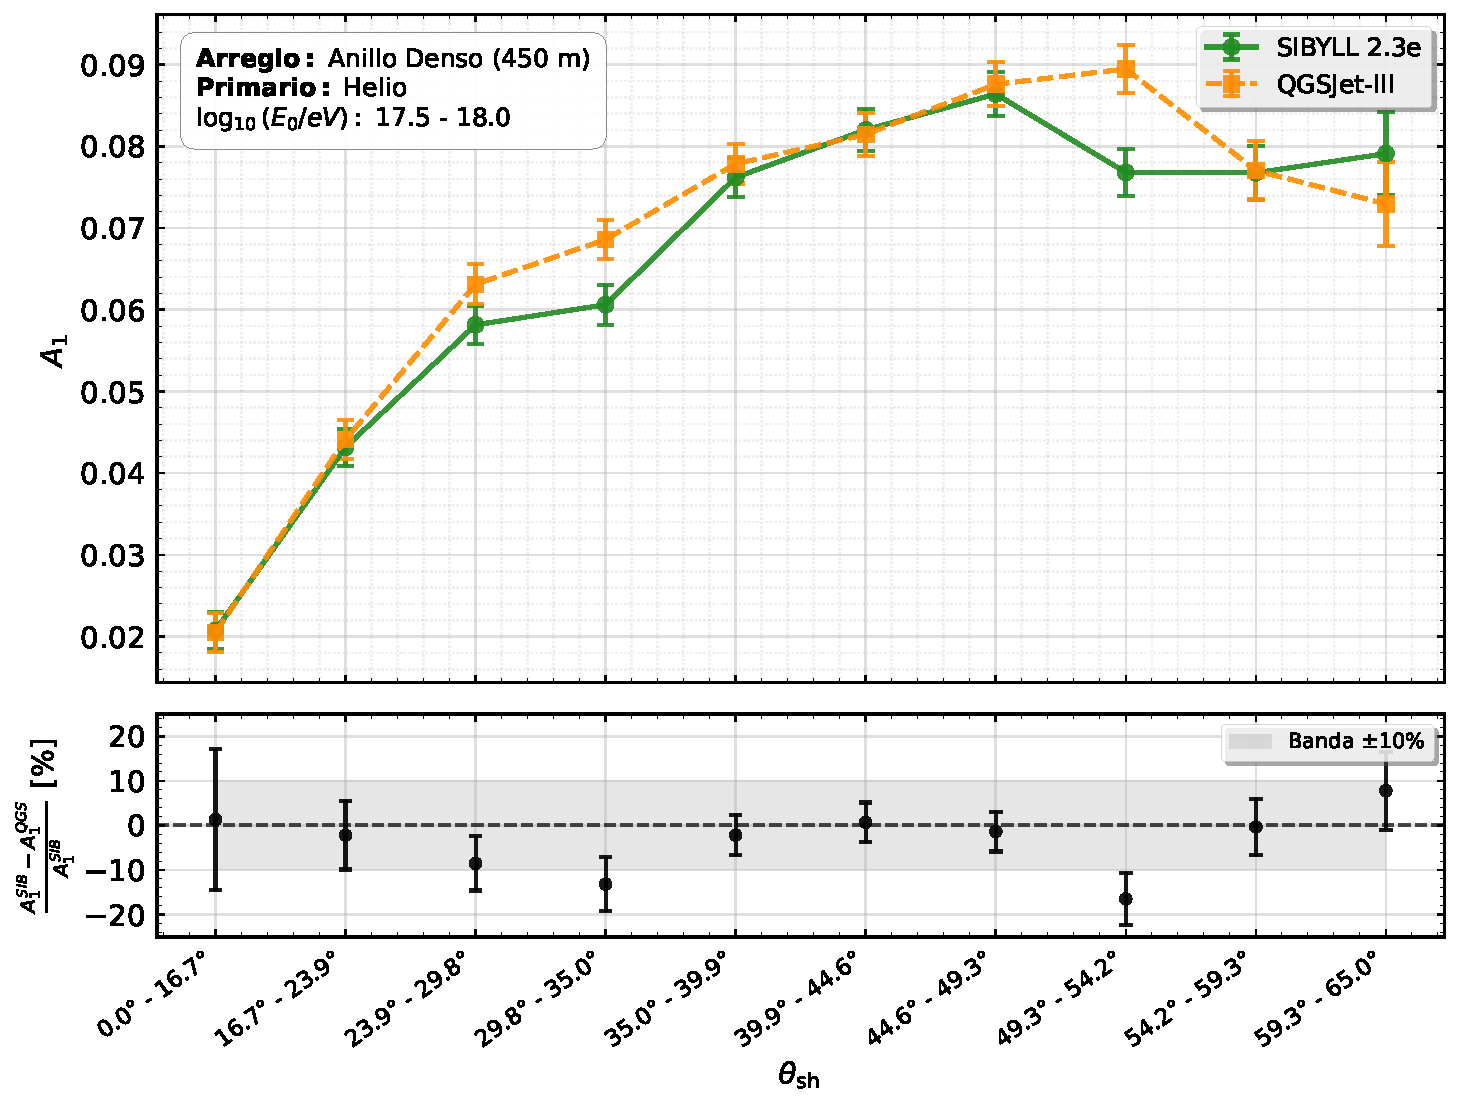
\includegraphics[width=\textwidth,height=4.3cm,keepaspectratio]{Hadronic_Uncertainty_Helium.pdf}
  \end{columns}
  \small
  \begin{itemize}
    \item $A_1$ no depende del azimut de arribo $\phi_{sh}$ (protones, $40^\circ$--$60^\circ$).
    \item SIBYLL~2.3e vs.\ QGSJET-III.01 (helio): diferencias relativas
      dentro de $\pm10\%$ en casi todo el rango. Comparación limitada a un
      primario.
  \end{itemize}
\end{frame}

\begin{frame}{Protón vs.\ hierro}
  \badgeAD
  \begin{columns}[c]
    \column{0.58\textwidth}
      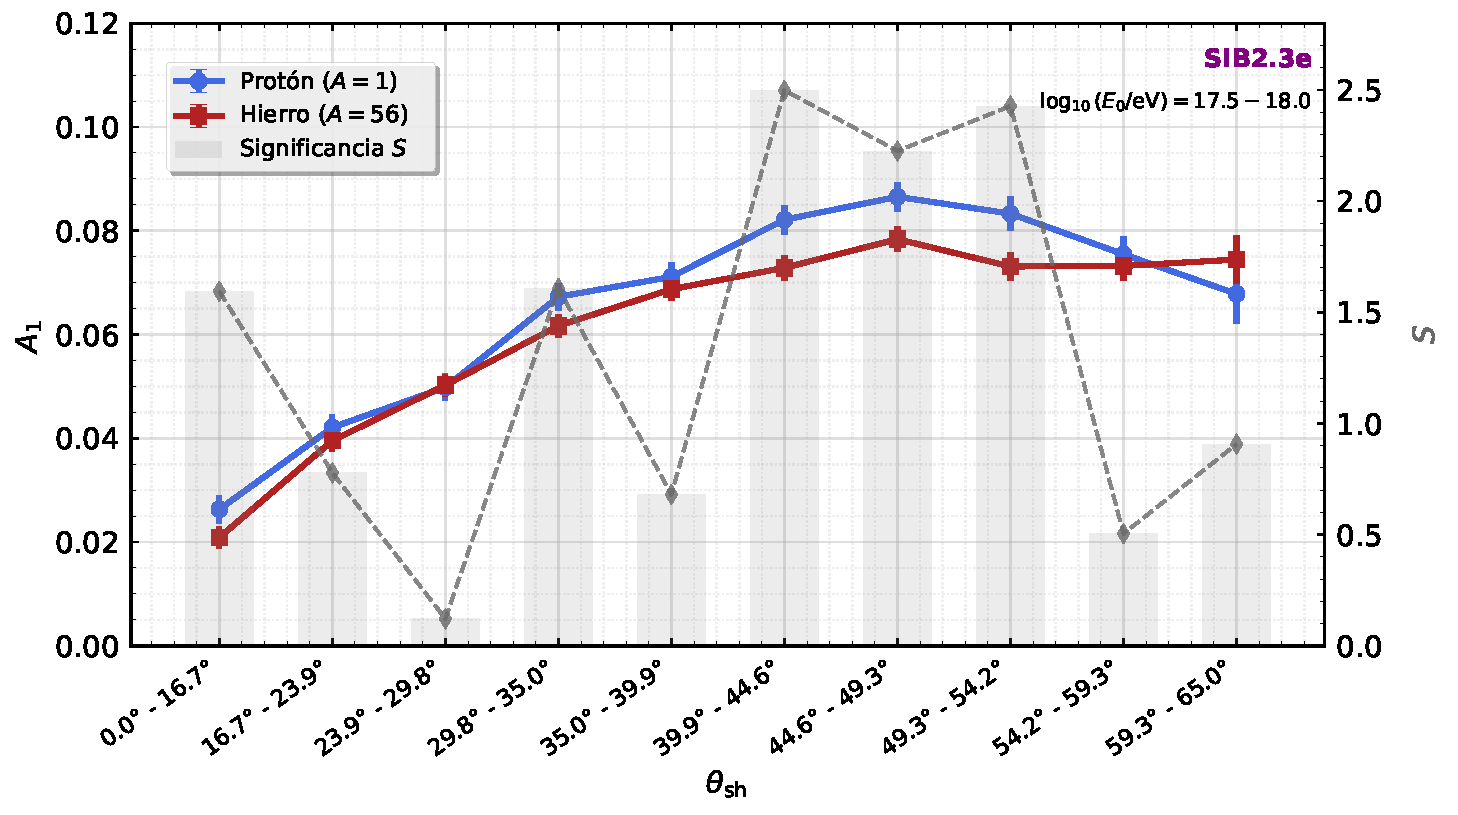
\includegraphics[width=\textwidth]{Mass_Discrimination_MF.pdf}
    \column{0.39\textwidth}
      \small
      \begin{itemize}
        \item $\langle A_1^{\text{p}}\rangle>\langle A_1^{\text{Fe}}\rangle$ en
          la mayoría de los bines.
        \item Significancia de la separación:
          \begin{equation*}
            S=\frac{|\langle A_1^{\text{p}}\rangle-\langle A_1^{\text{Fe}}\rangle|}
            {\sqrt{\sigma_{\text{p}}^2+\sigma_{\text{Fe}}^2}}
          \end{equation*}
        \item Máximo $S\sim2.5$ en $40^\circ$--$55^\circ$.
        \item $S$ es una diferencia de \textbf{medias}: crece como
          $\sqrt{N}$. No es una separación evento a evento.
      \end{itemize}
  \end{columns}
\end{frame}

\begin{frame}{Dependencia con la energía}
  \badgeAD
  \begin{columns}[c]
    \column{0.55\textwidth}
      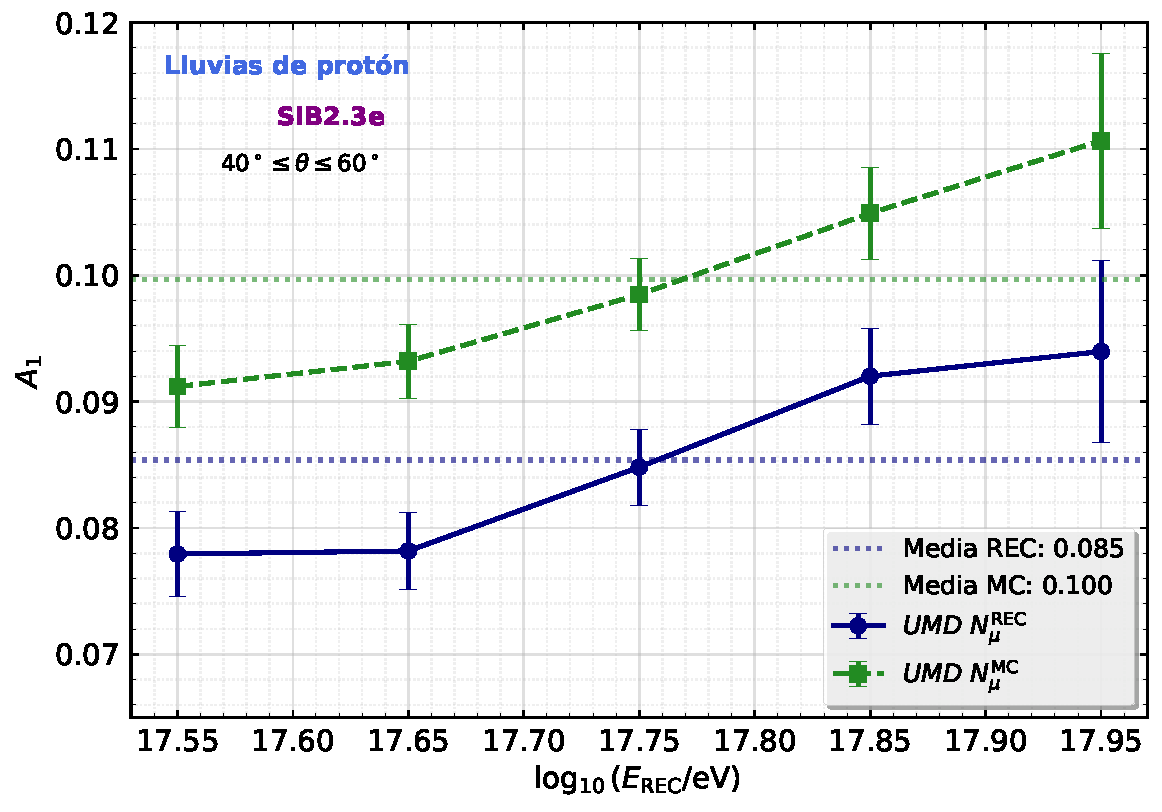
\includegraphics[width=\textwidth]{DenseRing_Systematics_Energy.pdf}
    \column{0.42\textwidth}
      \begin{itemize}
        \item Protones, $40^\circ$--$60^\circ$, 5 bines de energía reconstruida.
        \item $A_1$ crece levemente con $E$: $\Delta A_1\approx0.015$ en media
          década, igual en MC y en REC.
        \item Variación chica: justifica integrar todo el rango
          $[17.5,18.0)$ al comparar primarios.
      \end{itemize}
  \end{columns}
\end{frame}

\begin{frame}{Una interpretación común: el $X_{\max}$}
  \badgeHIP
  \setbeamerfont{itemize/enumerate body}{size=\footnotesize}
  \begin{columns}[c]
    \column{0.4\textwidth}
      \centering
      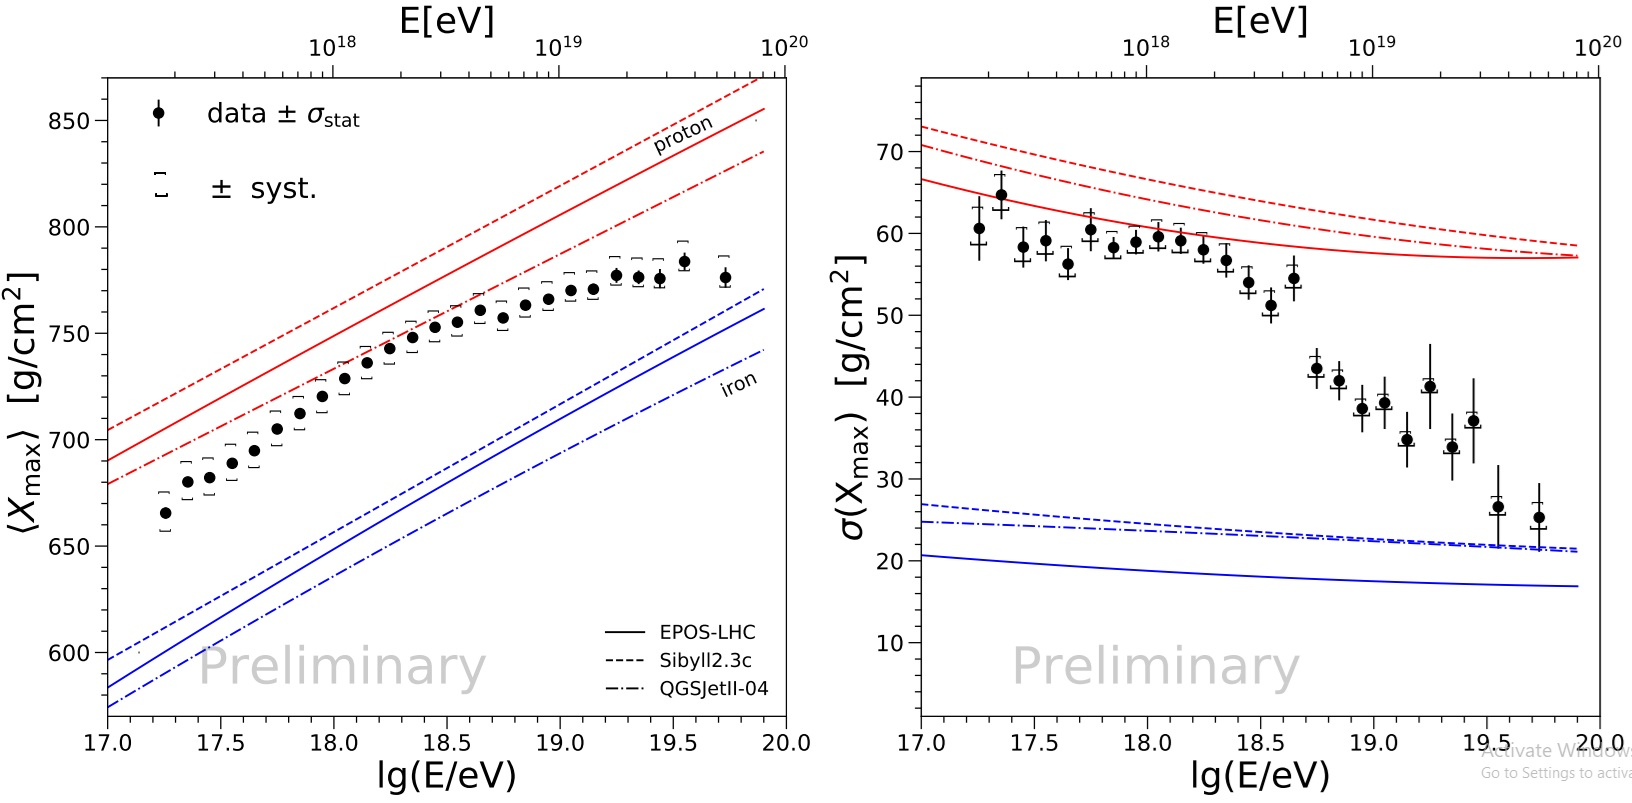
\includegraphics[width=\textwidth,height=4.3cm,keepaspectratio]{x_max.jpg}

      {\tiny Medición del FD de Auger, externa a este trabajo.}
    \column{0.57\textwidth}
      \footnotesize
      \begin{itemize}
        \item Medido por Auger: el $X_{\max}$ es más
          profundo a \textbf{mayor energía} y para \textbf{primarios
          livianos}.
        \item Acá: protón $>$ hierro y $A_1$ crece con $E$. En ambos casos,
          $X_{\max}$ más profundo.
        \item Lluvia más profunda $\Rightarrow$ los muones se producen
          \textbf{más cerca del suelo}: $D$ menor.
        \item La diferencia de camino entre temprana y tardía,
          $d_{\text{tardío}}-d_{\text{temprano}}\simeq2r\tan\theta_{sh}$,
          \textbf{no depende de $D$}: pesa más cuanto más chico es $D$.
        \item Esto se condice con el modelo linealizado, que va como
          $r/D$:\;
          $A_1\simeq\big[2-s+D/\lambda+\kappa\big]\frac{r}{D}\tan\theta_{sh}$
          $\Rightarrow$ \textbf{$A_1$ crece al bajar $D$}.
      \end{itemize}
  \end{columns}
  \fuente{Fuente: Yushkov \textit{et al.}, ICRC 2019.}
\end{frame}

\begin{frame}{¿Por qué el SD va al revés con el $X_{\max}$?}
  \badgeHIP
  \begin{columns}[c]
    \column{0.42\textwidth}
      \centering
      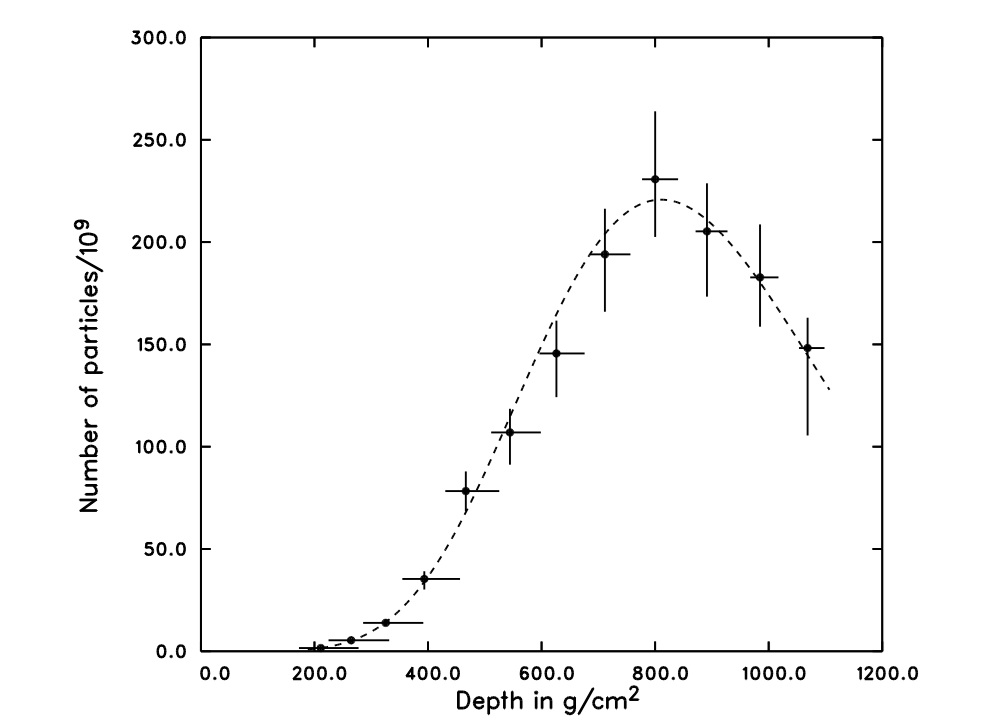
\includegraphics[width=\textwidth,height=4.4cm,keepaspectratio]{ammount_xmax.jpg}
      {\tiny Perfil longitudinal de un evento de Fly's Eye}
    \column{0.55\textwidth}
      \small
      \textbf{Componente EM (SD)} --- sigue el \emph{gradiente} del perfil:
      \begin{equation*}
        A_{EM}\propto\frac{1}{\rho_{EM}}\frac{\partial\rho_{EM}}{\partial X}\,\Delta X
      \end{equation*}
      Lluvia más profunda $\Rightarrow$ el suelo se acerca al máximo, donde
      $\partial\rho/\partial X\to0$ $\Rightarrow$ $A_{EM}$ \textbf{decrece}.

      \vspace{0.4em}
      \textbf{Componente muónica (UMD)} --- sigue la \emph{distancia}:
      $A_\mu\propto r/D$ $\Rightarrow$ $A_\mu$ \textbf{crece}.

      \vspace{0.4em}
      \alert{Tendencias opuestas con $X_{\max}$}, consistente con lo reportado
      para el SD (Bradfield 2022).
  \end{columns}
\end{frame}

% ============================================================
\section{El SD: una inversión de signo}
% ============================================================

\begin{frame}{El UMD en el arreglo \emph{Infill}}
  \badgeIF
  \begin{columns}[c]
    \column{0.62\textwidth}
      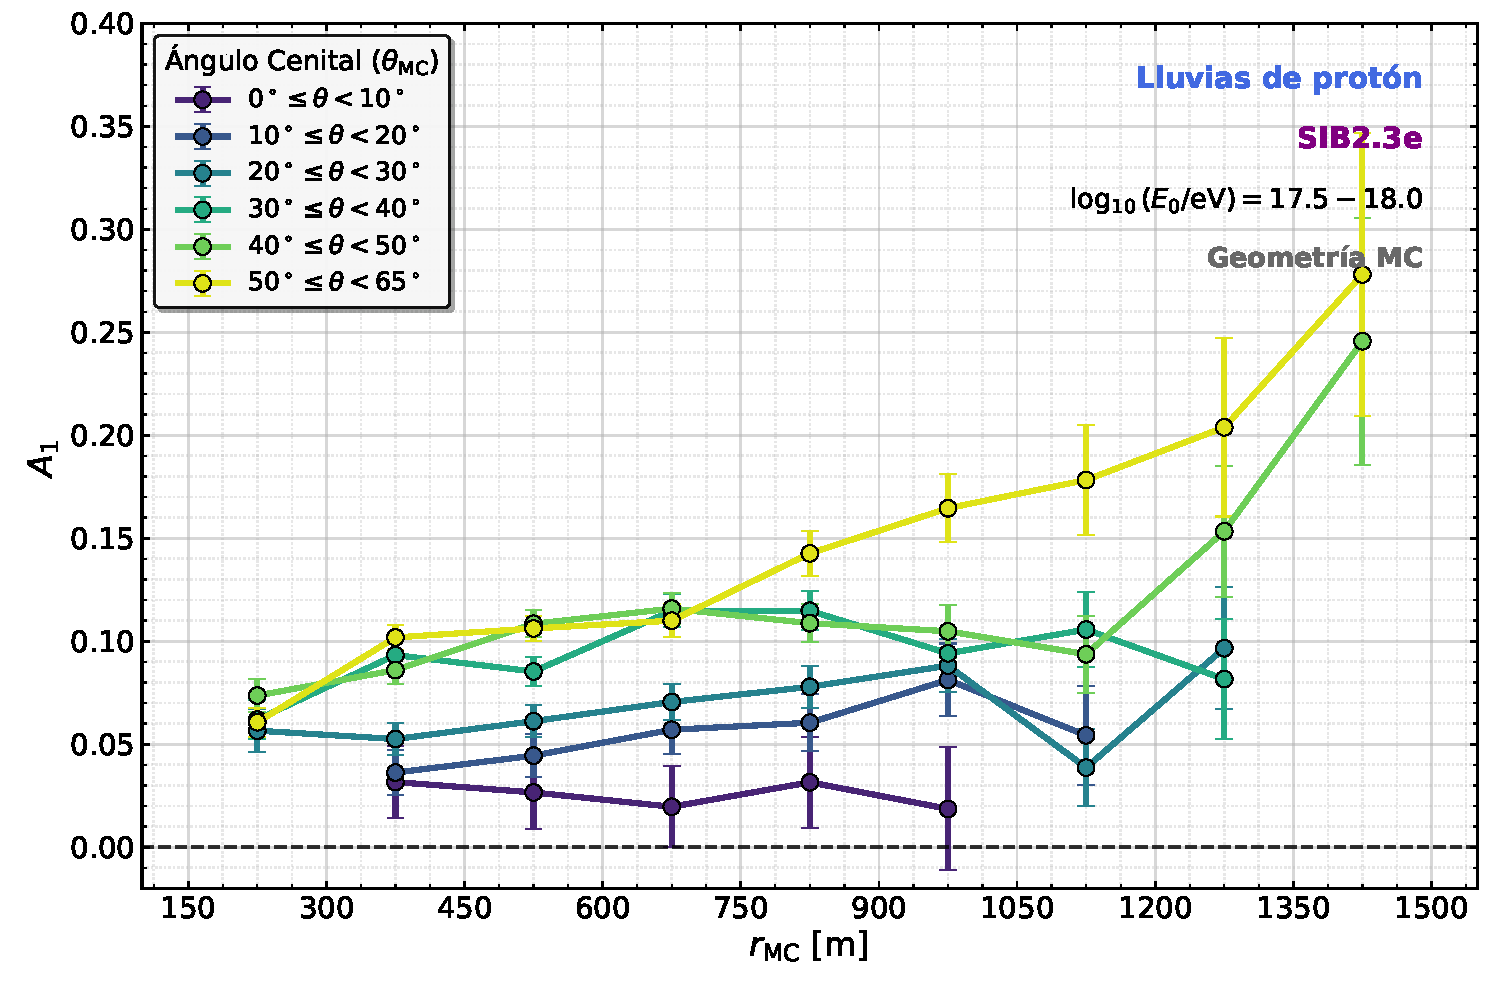
\includegraphics[width=\textwidth]{Global_A1_vs_R_Theta_MC.pdf}
    \column{0.35\textwidth}
      \small
      \begin{itemize}
        \item Geometría MC (núcleo y dirección verdaderos), bines de 150~m.
        \item $\theta<10^\circ$: compatible con cero.
        \item $10^\circ$--$40^\circ$: crece, con una meseta en
          $30^\circ$--$40^\circ$.
        \item $\theta\ge40^\circ$: crecimiento monótono hasta 1500~m.
        \item \textbf{Positiva y creciente con $r$ y $\theta$}: como el modelo.
      \end{itemize}
  \end{columns}
\end{frame}

\begin{frame}{UMD vs.\ señal total del SD}
  \badgeIF
  \setbeamerfont{itemize/enumerate body}{size=\footnotesize}
  \begin{columns}[c]
    \column{0.58\textwidth}
      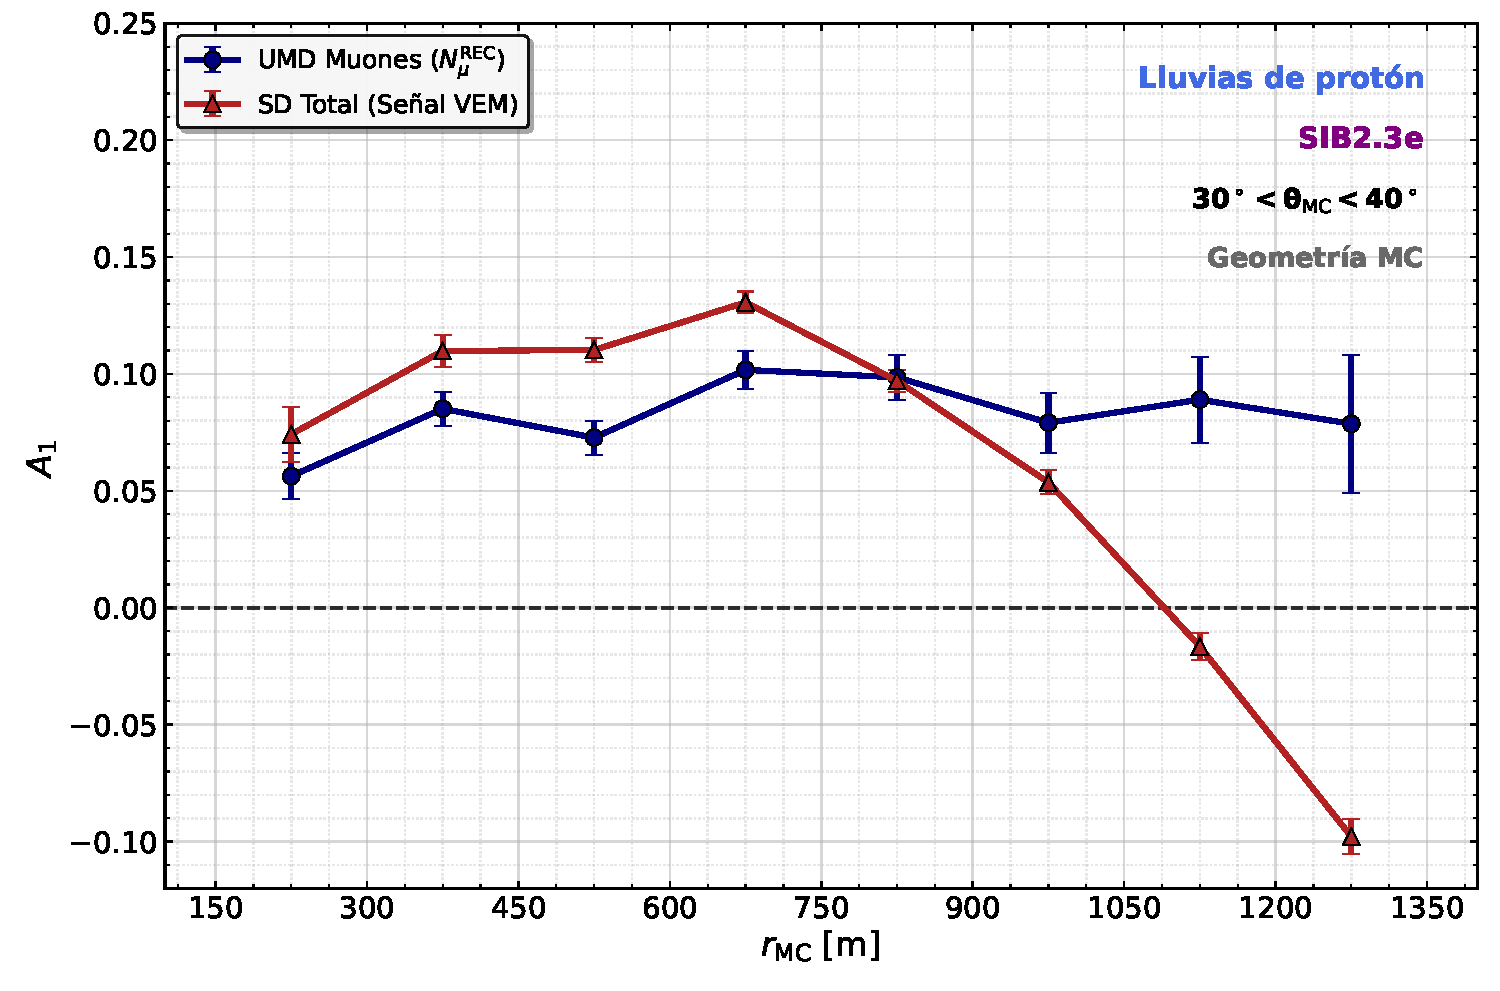
\includegraphics[width=\textwidth]{UMD_vs_SD_Total_Asymmetry.pdf}
    \column{0.39\textwidth}
      \footnotesize
      \begin{itemize}
        \item $30^\circ$--$40^\circ$, geometría MC.
        \item UMD: positiva a toda distancia.
        \item SD total: un máximo, decrece y \alert{se invierte} lejos del
          núcleo.
        \item Ya reportada para el SD (Bradfield 2022), sin explicación.
        \item Con geometría MC \textbf{no} es un error del núcleo ni de las
          coordenadas, ni una mezcla de las posiciones $\phi$ de las
          estaciones.
      \end{itemize}
  \end{columns}
\end{frame}

\begin{frame}[t]{Desglose de la señal del SD}
  \badgeIF
  \vspace{-1.4em}
  \setbeamerfont{itemize/enumerate body}{size=\footnotesize}
  \begin{columns}[T]
    \column{0.54\textwidth}
      \vspace{1.2em}
      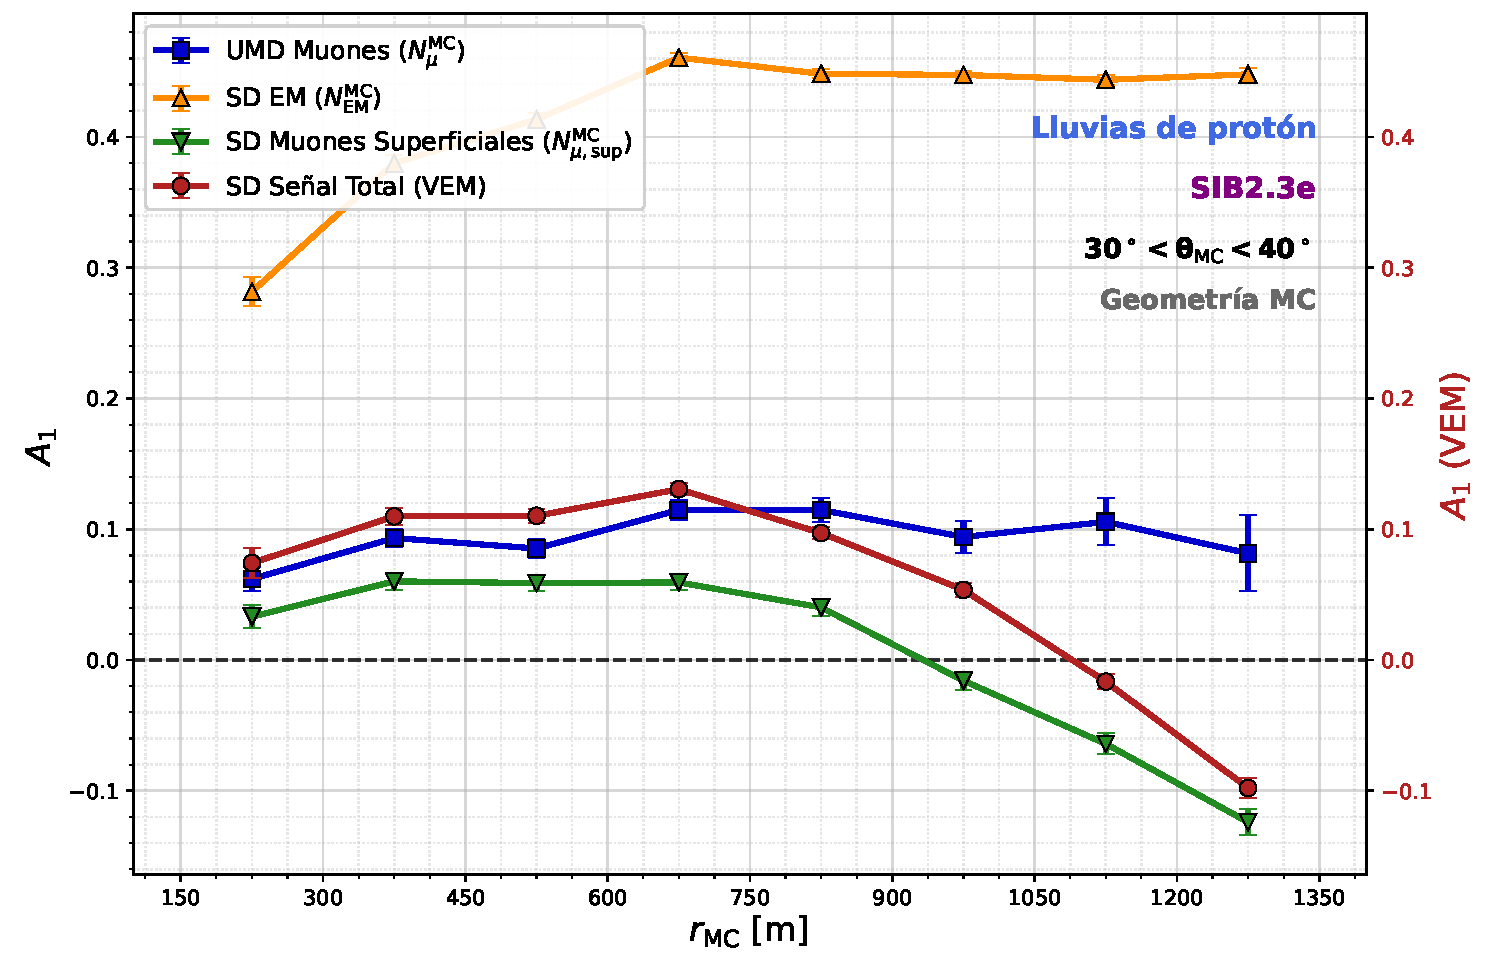
\includegraphics[width=\textwidth]{SD_Desglose_Componentes_vs_UMD.pdf}
    \column{0.44\textwidth}
      \footnotesize
      \begin{itemize}
        \item Conteos MC de partículas en el tanque, separados por componente.
        \item \textcolor{itedaOrange}{\textbf{EM}}: fuertemente positiva a todo $r$.
        \item \textcolor{plotGreen}{\textbf{Muones del SD}}: positivos cerca del
          núcleo; desde $\sim$600~m empiezan a disminuir y a partir de
          $\sim$900~m son \alert{negativos}.
        \item La \textbf{señal total del SD} sigue a sus muones a gran $r$.
      \end{itemize}
      \vspace{0.3em}
      \centering\alert{\textbf{Son los muones del SD los que se invierten.}}
  \end{columns}
\end{frame}

\begin{frame}<1-2>{¿Qué estamos viendo?}
  \badgeIF
  \setbeamerfont{itemize/enumerate body}{size=\footnotesize}
  \begin{columns}[c]
    \column{0.6\textwidth}
      \footnotesize
      \begin{itemize}
        \item \textbf{Es la misma lluvia}: un detector está enterrado debajo
          del otro.
        \item En ambos miramos \textbf{la misma cantidad}: los muones que
          atraviesan el detector (conteo MC).
        \item Fenomenologías completamente distintas:
        \begin{itemize}
          \item UMD: positiva y creciente $\Rightarrow$ \textbf{coincide con el
            modelo}.
          \item SD: se invierte $\Rightarrow$ \textbf{no coincide}.
        \end{itemize}
      \end{itemize}
      \vspace{0.3em}
      \visible<2>{%
        \begin{alertblock}{Preguntas}
          ¿Nos faltó algo en la fenomenología? ¿Hay un fenómeno físico que
          no consideramos? ¿O es otra cosa?
        \end{alertblock}%
      }
    \column{0.37\textwidth}
      \centering
      \visible<2>{%
        
\includegraphics[width=\textwidth, trim={0 245 0 245}, clip]{confused_physics_meme.jpg}%
      }
  \end{columns}
\end{frame}

% ============================================================
\section{El sesgo de selección del SD}
% ============================================================

\begin{frame}{¿Cuándo dispara una estación del SD?}
  \begin{columns}[c]
    \column{0.55\textwidth}
      \begin{itemize}
        \item Las partículas que atraviesan el tanque emiten \textbf{luz
          Cherenkov} en el agua.
        \item Tres \textbf{PMTs} recogen esa luz. La señal se mide en
          \textbf{VEM}: la de un muón vertical que cruza el tanque entero.
        \item Si la señal supera un \textbf{umbral mínimo}, la estación
          \textbf{dispara} y puede formar parte de la reconstrucción del
          evento.
        \item El umbral es del orden de la señal de un muón vertical
          (\textbf{1 VEM}): un único muón puede no alcanzarlo.
      \end{itemize}
    \column{0.42\textwidth}
      \centering
      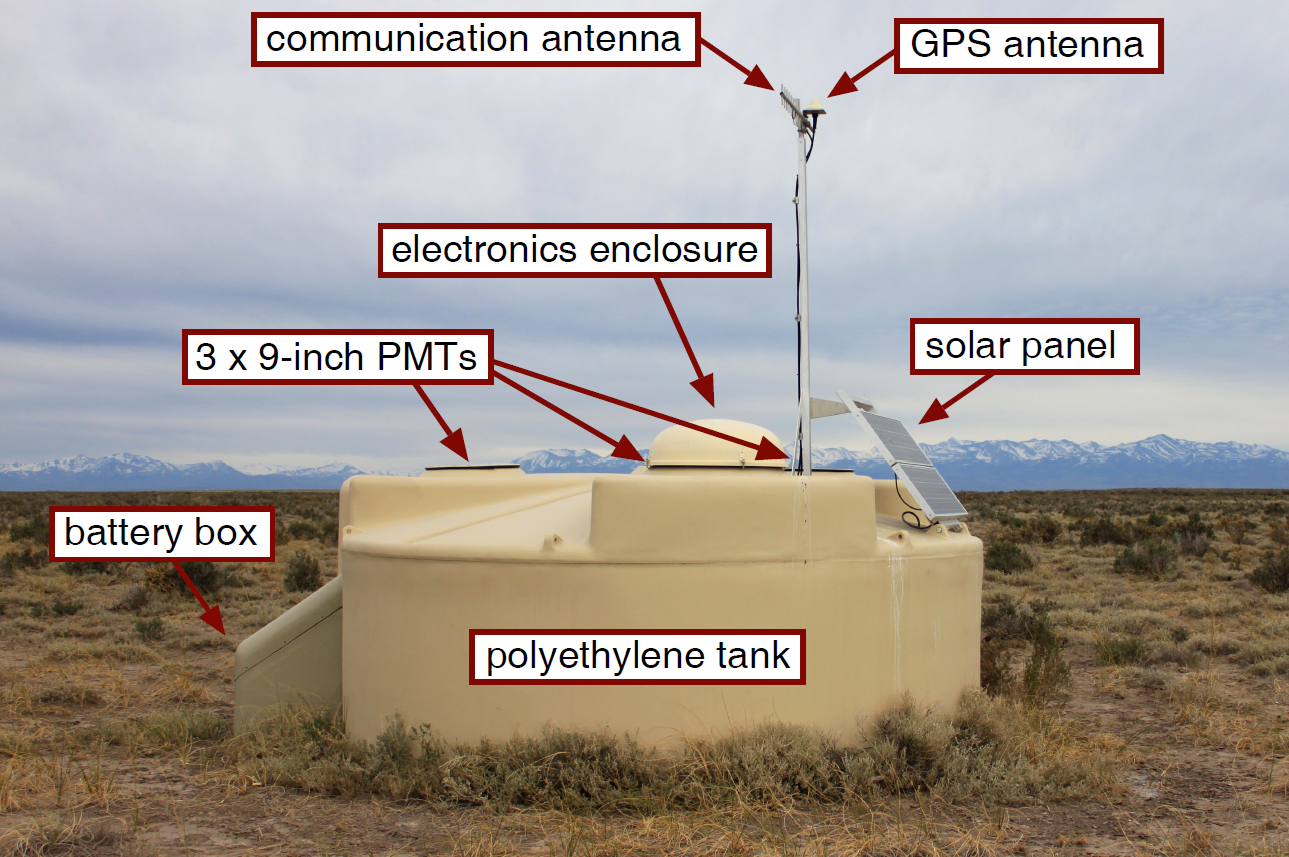
\includegraphics[width=\textwidth,height=5.0cm,keepaspectratio]{ssd.png}
  \end{columns}
\end{frame}

\begin{frame}{La hipótesis: qué estaciones entran al promedio}
  \badgeHIP
  \small
  El análisis promedia sólo las estaciones que \textbf{dispararon y forman
  parte del evento reconstruido}. Si la probabilidad de entrar depende del
  contenido de muones de la estación, y de forma distinta en cada región,
  el promedio se sesga.
  \vspace{0.3em}
  \begin{center}
  \begin{tikzpicture}[x=0.95cm,y=0.95cm,
      tank/.style={draw=itedaTealDark, minimum width=0.8cm, minimum height=0.6cm, rounded corners=1pt, font=\small\bfseries},
      on/.style={tank, fill=itedaTeal!35},
      off/.style={tank, fill=white, dashed, text=itedaGray}]
    \node[font=\small\bfseries, anchor=west] at (-0.4,1.2) {Región temprana (mucha EM)};
    \foreach \x/\n in {0/0,1/1,2/1,3/2,4/3} {\node[on] at (\x,0.4) {\n};}
    \node[font=\small, anchor=west, align=left] at (4.7,0.4) {verdadera: $1.4$\\ seleccionada: $1.4$};
    \node[font=\small\bfseries, anchor=west] at (-0.4,-0.6) {Región tardía (EM atenuada)};
    \foreach \x/\n in {0/0,1/0,2/1} {\node[off] at (\x,-1.4) {\n};}
    \foreach \x/\n in {3/2,4/2} {\node[on] at (\x,-1.4) {\n};}
    \node[font=\small, anchor=west, align=left] at (4.7,-1.4) {verdadera: $1.0$\\ seleccionada: \textcolor{plotMaroon}{$\mathbf{2.0}$}};
    \node[on, minimum width=0.5cm] at (8.6,0.4) {};
    \node[font=\scriptsize, anchor=west] at (8.95,0.4) {dispara};
    \node[off, minimum width=0.5cm] at (8.6,-0.3) {};
    \node[font=\scriptsize, anchor=west] at (8.95,-0.3) {no dispara};
    \node[font=\scriptsize, anchor=west] at (8.3,-1.0) {número = muones};
  \end{tikzpicture}
  \end{center}
  \vspace{-0.2em}
  \begin{itemize}
    \item Del lado tardío, una estación sólo entra si tiene \textbf{más muones
      que la media}: la media seleccionada sube y \alert{$A_1$ se invierte}
      sin crear ni mover ningún muón. (Ejemplo ilustrativo.)
  \end{itemize}
\end{frame}

\begin{frame}{Prueba 1: sacando la selección de estaciones}
  \badgeIF
  \vspace{-1.2em}
  \setbeamerfont{itemize/enumerate body}{size=\footnotesize}
  \begin{columns}[c]
    \column{0.52\textwidth}
      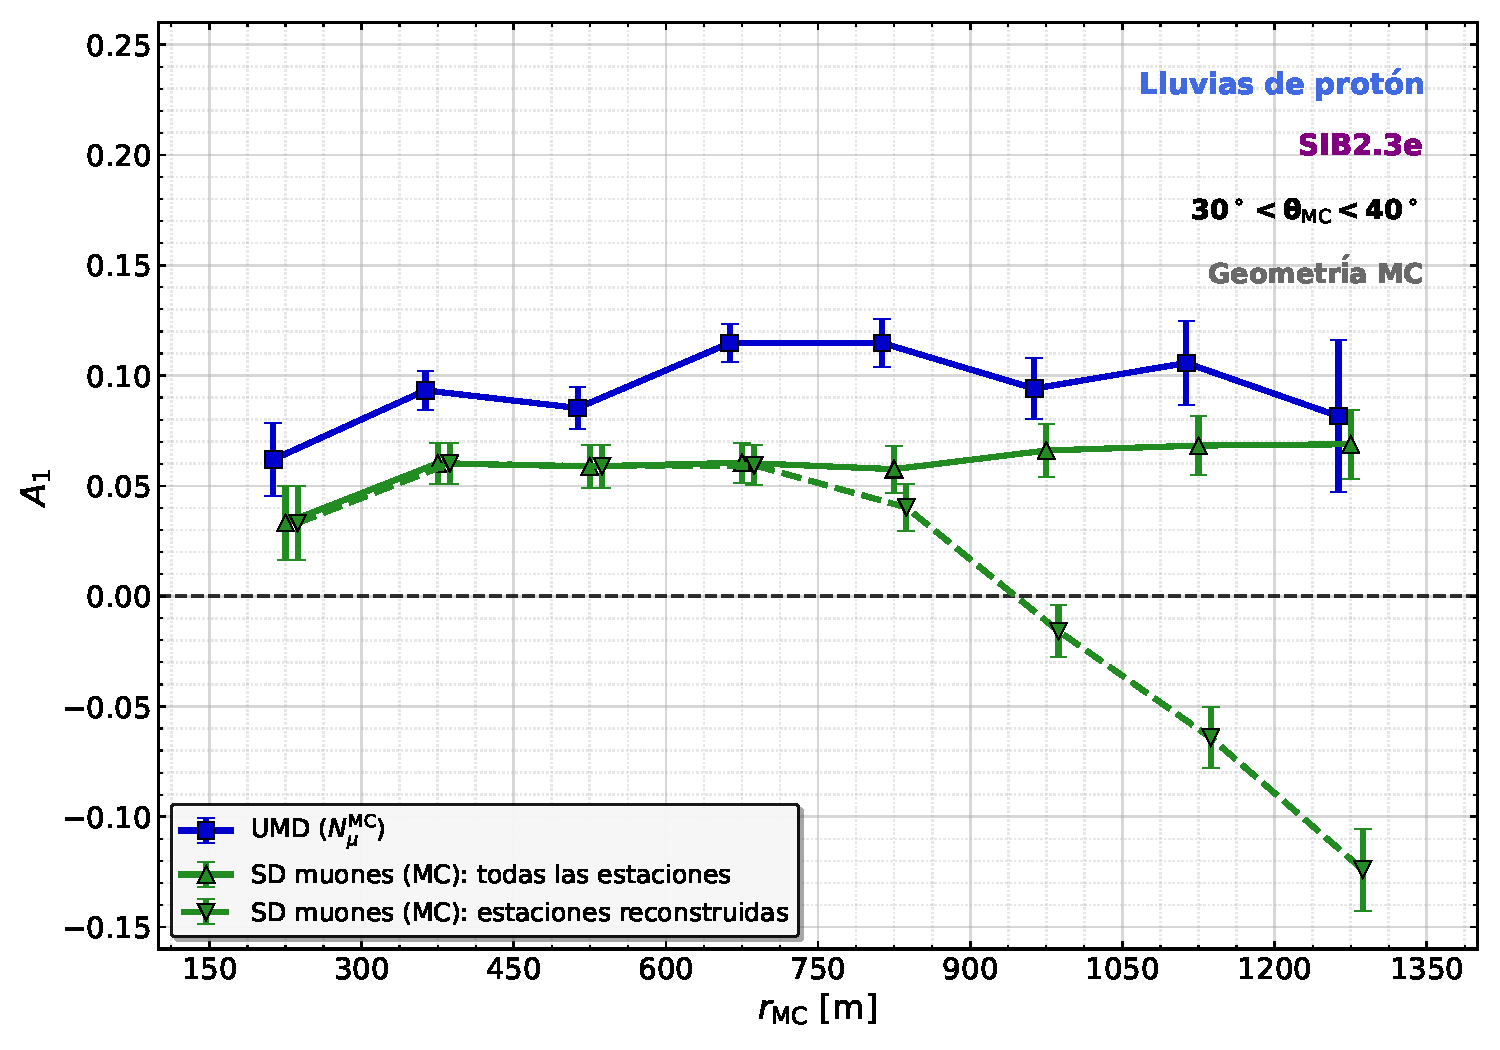
\includegraphics[width=\textwidth]{SD_Seleccion_Estaciones_vs_UMD.pdf}
    \column{0.46\textwidth}
      \small
      \begin{itemize}
        \item Mismos conteos, coordenadas y ajuste: sólo cambia \textbf{qué
          estaciones} entran al promedio.
        \item Sobre todas las estaciones, \textbf{la inversión desaparece}:
          los muones del SD se comportan como en el UMD, positivos a todo $r$.
        \item En $1200$--$1350$~m:
          \begin{center}
          \begin{tabular}{lc}
            \toprule
            todas & $+0.069\pm0.016$\\
            seleccionadas & \textcolor{plotMaroon}{$-0.124\pm0.019$}\\
            \bottomrule
          \end{tabular}
          \end{center}
      \end{itemize}
  \end{columns}
\end{frame}

\begin{frame}{Prueba 2: los tanques que quedan afuera}
  \badgeIF
  \centering
  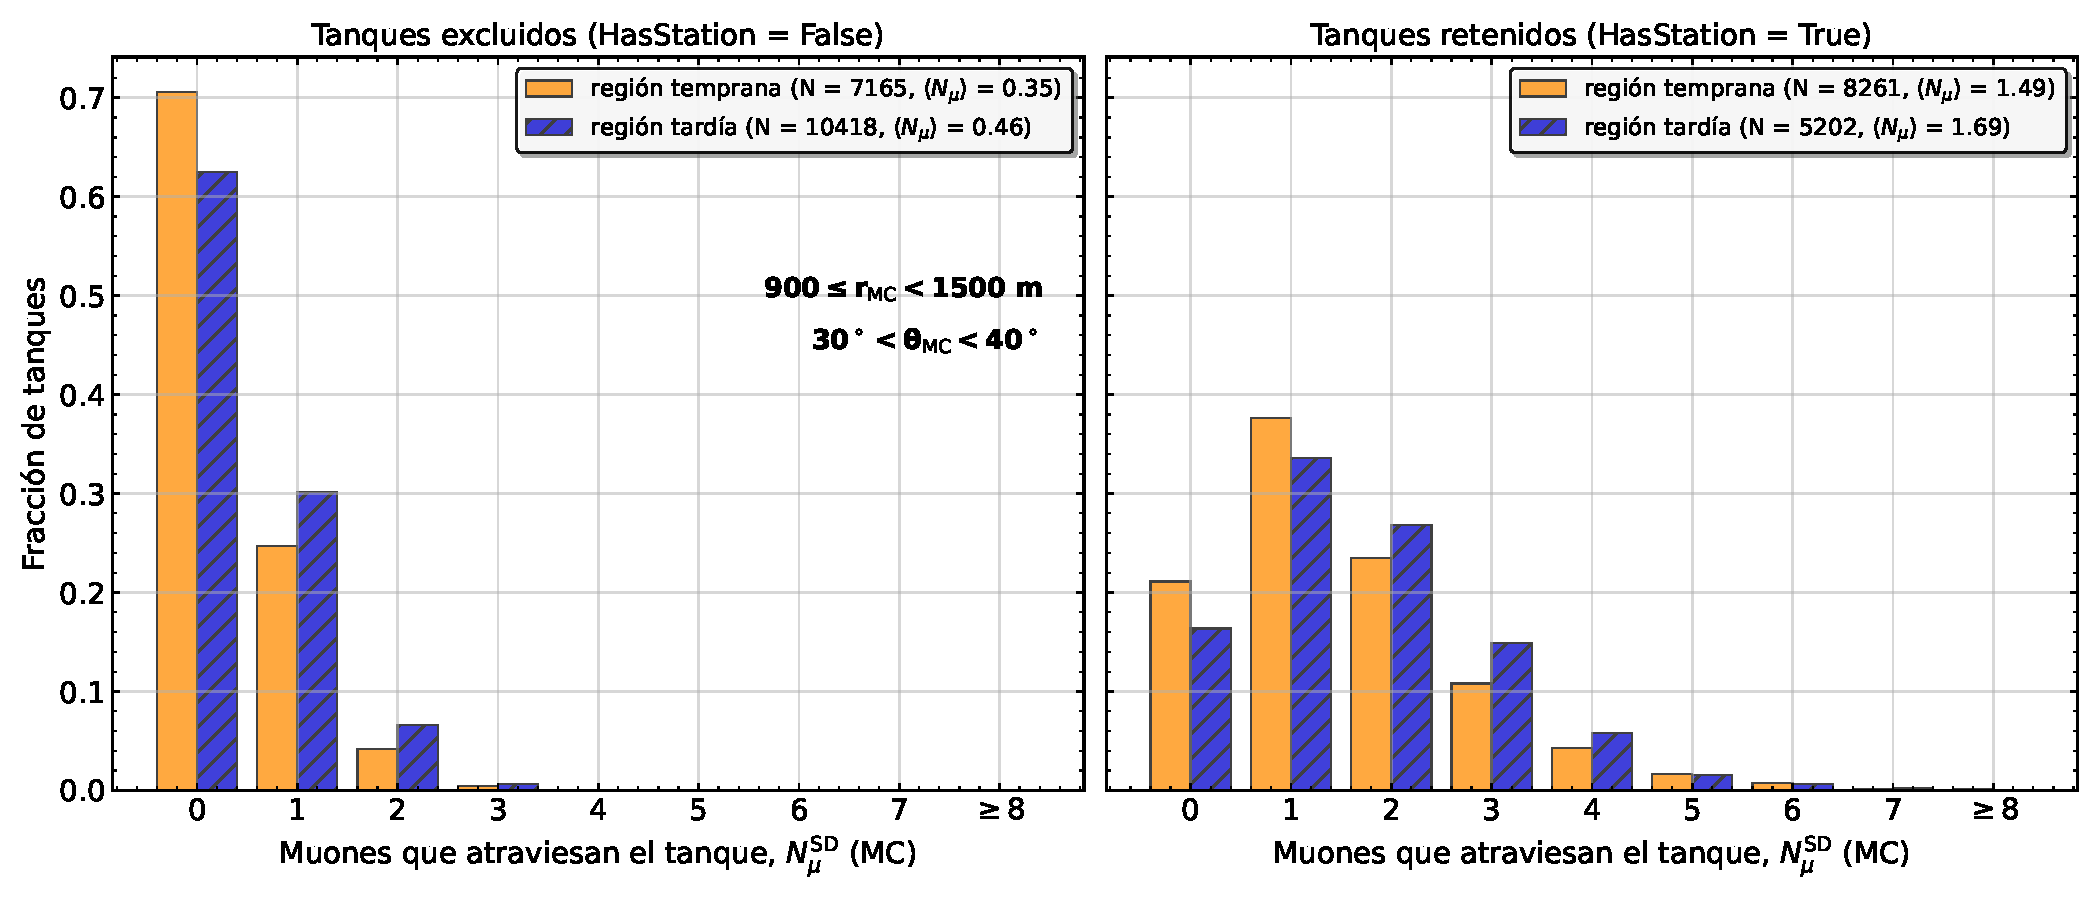
\includegraphics[width=\textwidth,height=3.3cm,keepaspectratio]{SD_Muones_Tanques_Excluidos.pdf}
  \begin{columns}[T]
    \column{0.5\textwidth}
      \small
      \begin{itemize}
        \item Si es selección, los tanques excluidos deben tener \textbf{muy
          pocos muones}: a lo sumo uno.
        \item Excluidos con $\le1$ muón: \alert{95\%} (temprana) y
          \alert{93\%} (tardía).
      \end{itemize}
    \column{0.47\textwidth}
      \small
      \begin{itemize}
        \item Media de los excluidos: $0.35$ y $0.46$ muones.
        \item \textbf{Lo esperado}: la hipótesis gana plausibilidad.
      \end{itemize}
  \end{columns}
  \fuente{Temprana $|\phi|<60^\circ$, tardía $|\phi|>120^\circ$.}
\end{frame}

\begin{frame}{¿Qué estaciones entran, en cada región?}
  \badgeIF
  \setbeamerfont{itemize/enumerate body}{size=\footnotesize}
  \vspace{-1.4em}
  \begin{center}
    \footnotesize
    \renewcommand{\arraystretch}{1.0}
    \begin{tabular}{lcc}
      \toprule
      & \textbf{Temprana} & \textbf{Tardía}\\
      \midrule
      De cada 100 estaciones, forman parte del evento & $42$ & $18$\\
      \midrule
      Muones medios en las que \textbf{entran} & $1.49$ & \textcolor{plotMaroon}{$\mathbf{1.69}$}\\
      Muones medios en las que \textbf{quedan afuera} & $0.35$ & $0.46$\\
      \midrule
      Partículas EM medias en las que quedan afuera & $28$ & $14$\\
      \bottomrule
    \end{tabular}
  \end{center}
  \vspace{-0.3em}
  \begin{enumerate}
    \item Del lado tardío \textbf{entran muchas menos estaciones}: 18 de cada
      100, contra 42 del temprano.
    \item Las que entran tienen \textbf{más muones que la media de su región},
      y del lado tardío el exceso es mucho mayor: las tardías que entran
      tienen incluso más muones que las tempranas $\Rightarrow$ el promedio
      sobreestima la región tardía y \alert{$A_1$ se invierte ($A_1<0$)}.
    \item \textbf{Hipótesis}: del lado tardío queda muy poca componente EM y
      cuesta mucho que una estación dispare $\Rightarrow$ sólo entran las que
      tienen \textbf{mucha más componente muónica que la media} de su región.
  \end{enumerate}
\end{frame}

\begin{frame}{Qué queda abierto}
  \badgeIF
  \begin{itemize}
    \item Sin selección, los muones del SD recuperan el signo positivo, pero
      \textbf{no igualan al UMD}: entre 150 y 900~m el UMD es mayor en
      $0.03$--$0.06$.
    \item Candidata, ya en el modelo: la respuesta de placa ($\kappa=1$) frente
      a la del tanque, y el umbral del UMD más alto del lado tardío.
    \item La curva del UMD también usa estaciones seleccionadas: el UMD
      \textbf{no tiene trigger propio}, entra si dispara el tanque de su
      estación. El efecto debería ser menor (los muones enterrados no hacen
      disparar al tanque), pero no puede descartarse a grandes distancias.
  \end{itemize}
  \begin{block}{Conclusión}
    La asimetría del conteo de muones depende de la respuesta del detector
    \textbf{y} de la selección de estaciones. Toda comparación entre detectores,
    o entre simulaciones y datos, exige la misma selección.
  \end{block}
\end{frame}

% ============================================================
\section{¿Por qué la reconstrucción reduce la asimetría del UMD?}
% ============================================================

\begin{frame}{La pregunta}
  \badgeAD
  \begin{columns}[c]
    \column{0.58\textwidth}
      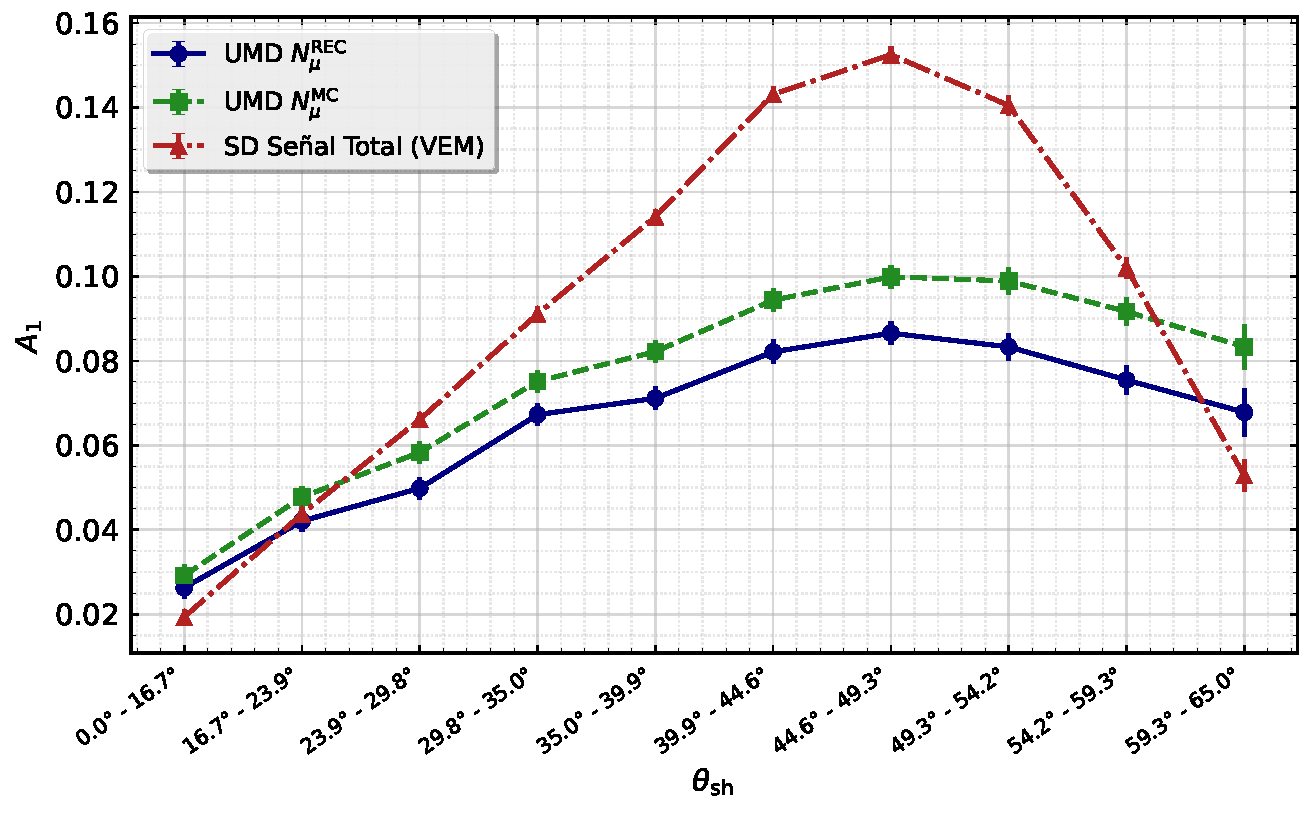
\includegraphics[width=\textwidth]{Evolucion_Asimetria_vs_Theta.pdf}
    \column{0.39\textwidth}
      \begin{itemize}
        \item UMD REC: \textbf{misma forma}, \textbf{menor amplitud} que UMD MC.
        \item Lo único que cambia es la reconstrucción.
        \item ``La reconstrucción baja la asimetría'' no explica nada:
          \alert{¿cuál es el efecto?}
      \end{itemize}
  \end{columns}
\end{frame}

\begin{frame}{¿Es un problema de los ajustes?}
  \badgeAD
  \begin{columns}[c]
    \column{0.58\textwidth}
      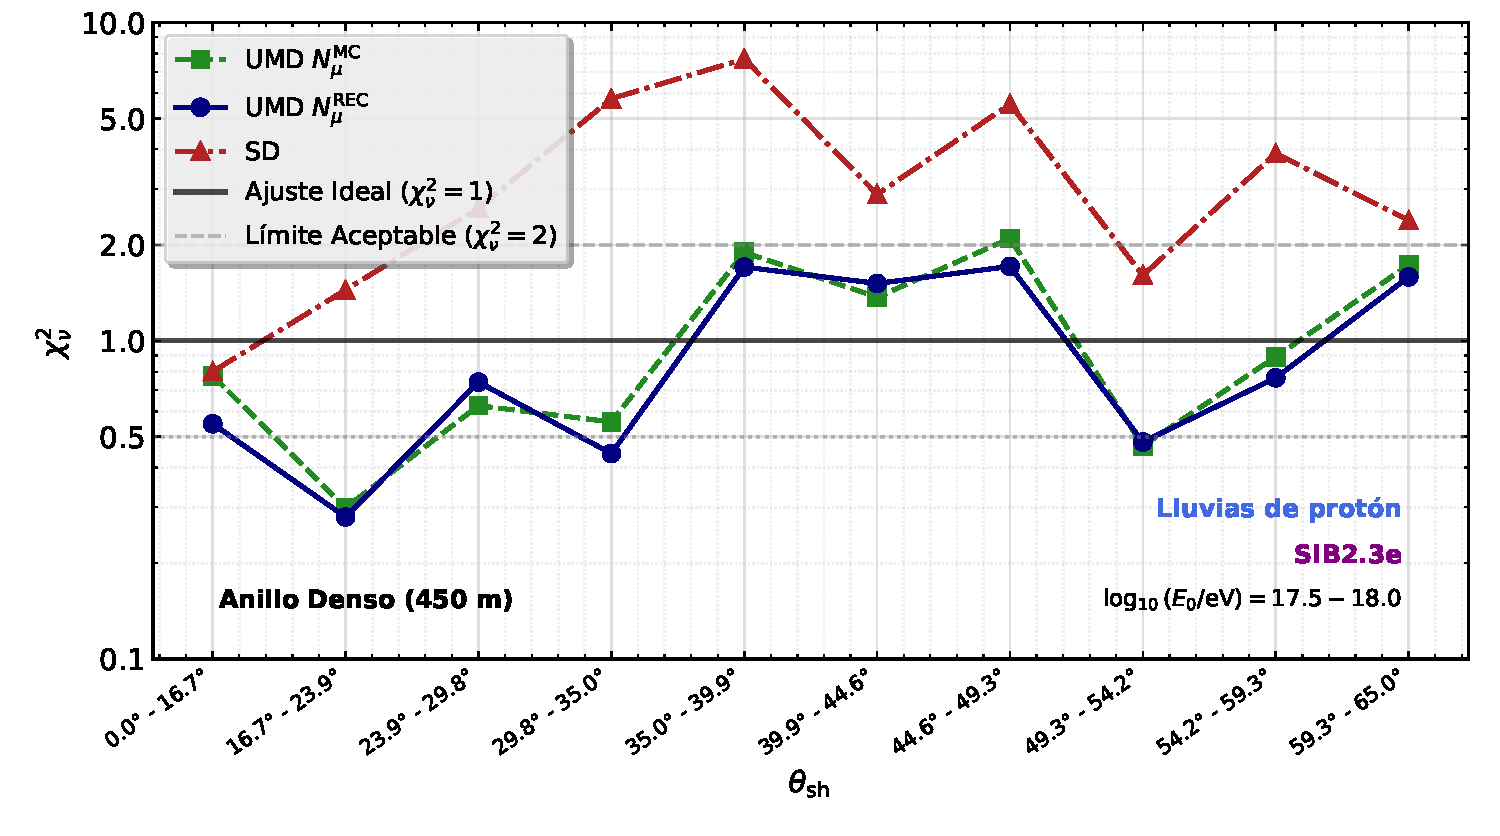
\includegraphics[width=\textwidth]{Chi2_Reduced_Fits.pdf}
    \column{0.39\textwidth}
      \small
      \begin{itemize}
        \item Hipótesis: ajustes peores $\Rightarrow$ amplitud más chica.
        \item UMD, MC y REC: $\chi^2_\nu\approx1$. \textbf{Se descarta.}
        \item Al margen, el SD: $\chi^2_\nu$ hasta $\sim10$. Con errores tan
          chicos, el ajuste se vuelve sensible a lo que el modelo no incluye
          (armónicos superiores, correlación entre estaciones de una misma
          lluvia).
      \end{itemize}
  \end{columns}
\end{frame}

\begin{frame}{El residuo de la reconstrucción de muones}
  \badgeAD
  \begin{columns}[c]
    \column{0.52\textwidth}
      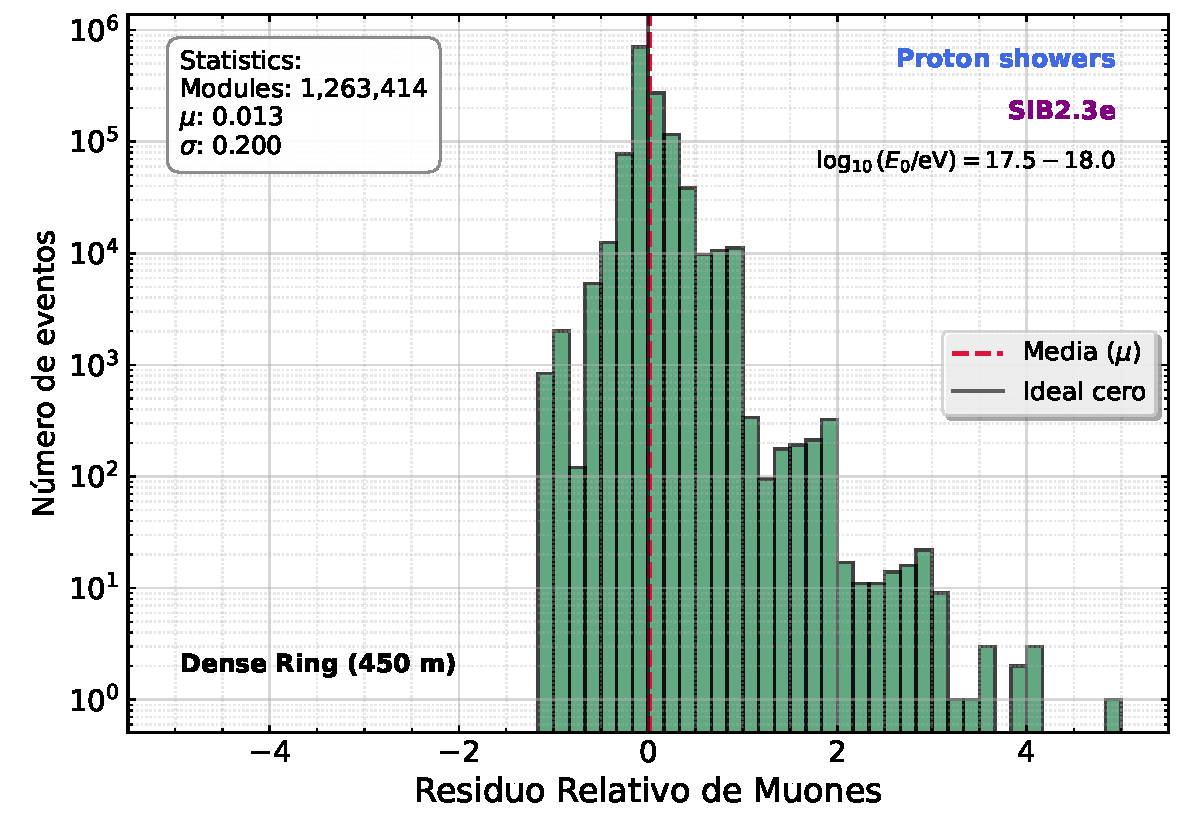
\includegraphics[width=\textwidth]{muon_counting_validation.pdf}
    \column{0.45\textwidth}
      \small
      \begin{equation*}
        \text{Residuo}=\frac{N_\mu^{\text{REC}}-N_\mu^{\text{MC}}}{N_\mu^{\text{MC}}}
      \end{equation*}
      \begin{itemize}
        \item Media $\approx0.013$, ancho $\sigma\approx0.20$: \textbf{casi
          sin sesgo}. Un problema difícil de encontrar.
        \item Pero \textbf{no es simétrica}: con 1 muón, lo mínimo es
          reconstruir 0 (residuo $-1$); hacia arriba, 2, 3, 4\ldots\ sin cota.
        \item \emph{Bootstrap} sorteando de esta distribución global:
          \alert{no reproduce} $A_1^{\text{REC}}$, sólo agrega ruido.
      \end{itemize}
  \end{columns}
\end{frame}

\begin{frame}{El error depende de la región}
  \badgeAD
  \begin{columns}[c]
    \column{0.55\textwidth}
      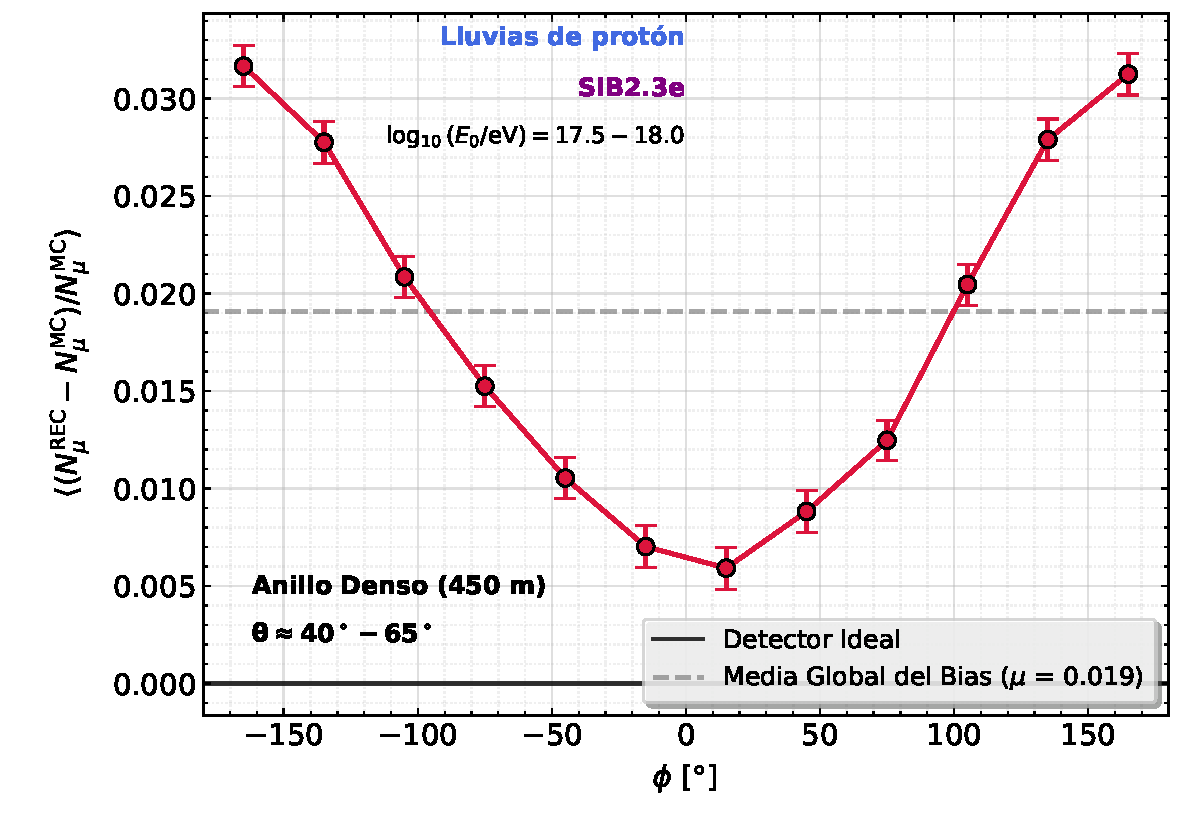
\includegraphics[width=\textwidth]{directional_bias.pdf}
    \column{0.42\textwidth}
      \small
      \begin{itemize}
        \item Hipótesis: el error no es igual en la región temprana que en la
          tardía.
        \item Media del residuo vs.\ $\phi$: $\approx0.005$ en la temprana,
          $\approx0.03$ en la tardía.
        \item Son \textbf{medias} de distribuciones con la misma forma
          asimétrica, no gaussianas.
        \item Más sobreconteo donde hay menos muones $\Rightarrow$ sube el
          ``piso'' tardío $\Rightarrow$ \textbf{baja $A_1$}.
      \end{itemize}
  \end{columns}
\end{frame}

\begin{frame}{\emph{Bootstrap} con la distribución de cada región}
  \badgeAD
  \begin{columns}[c]
    \column{0.58\textwidth}
      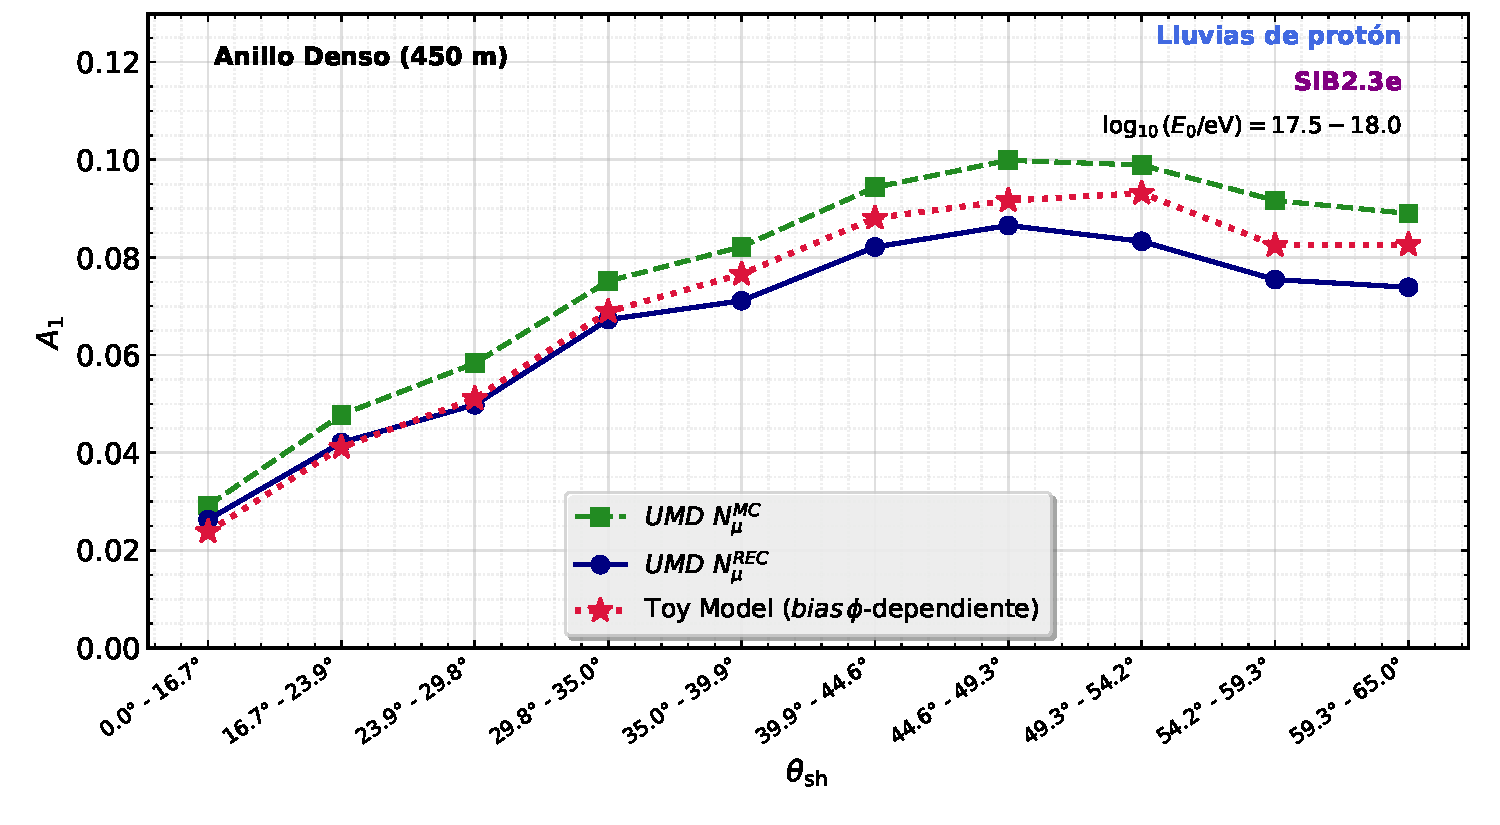
\includegraphics[width=\textwidth]{toy_model.pdf}
    \column{0.39\textwidth}
      \small
      \begin{itemize}
        \item A cada estación con $N_\mu^{\text{MC}}$ se le asigna un residuo
          sorteado de la distribución de \textbf{su} región azimutal.
        \item $\theta\lesssim35^\circ$: reproduce $A_1^{\text{REC}}$
          \textbf{por completo}.
        \item $\theta\gtrsim35^\circ$: explica más de la mitad de la pérdida.
        \item El remanente queda \alert{abierto}.
      \end{itemize}
  \end{columns}
\end{frame}

\begin{frame}[t]{En el arreglo real: una segunda reconstrucción}
  \badgeIF
  \vspace{-1.2em}
  \begin{itemize}
    \item En el Anillo Denso las estaciones están fijas a 450~m del núcleo
      verdadero. En el \emph{Infill}, $r$ y $\phi$ de cada estación se
      calculan con el \textbf{núcleo y la dirección reconstruidos}.
    \item Calculamos la asimetría $A_1$ del \textbf{mismo} número de muones
      inyectado ($450\le r<600$~m) con las dos geometrías: la
      \textbf{verdadera} (MC) y la \textbf{reconstruida} (REC).
  \end{itemize}
  \begin{center}
    \renewcommand{\arraystretch}{1.1}
    \begin{tabular}{lcc}
      \toprule
      $\theta_{sh}$ & $A_1$, geometría MC & $A_1$, geometría REC\\
      \midrule
      $20^\circ$--$30^\circ$ & $0.062$ & $0.011$\\
      $30^\circ$--$40^\circ$ & $0.086$ & $0.002$\\
      $40^\circ$--$50^\circ$ & $0.108$ & \textcolor{plotMaroon}{$-0.002$}\\
      \bottomrule
    \end{tabular}
  \end{center}
  \begin{itemize}
    \item Con la geometría reconstruida la asimetría \textbf{desaparece casi
      por completo}: mucho más que lo que explica el conteo.
  \end{itemize}
\end{frame}

\begin{frame}{El núcleo reconstruido se corre hacia la temprana}
  \badgeIF
  \vspace{-1.8em}
  \setbeamerfont{itemize/enumerate body}{size=\footnotesize}
  \centering
  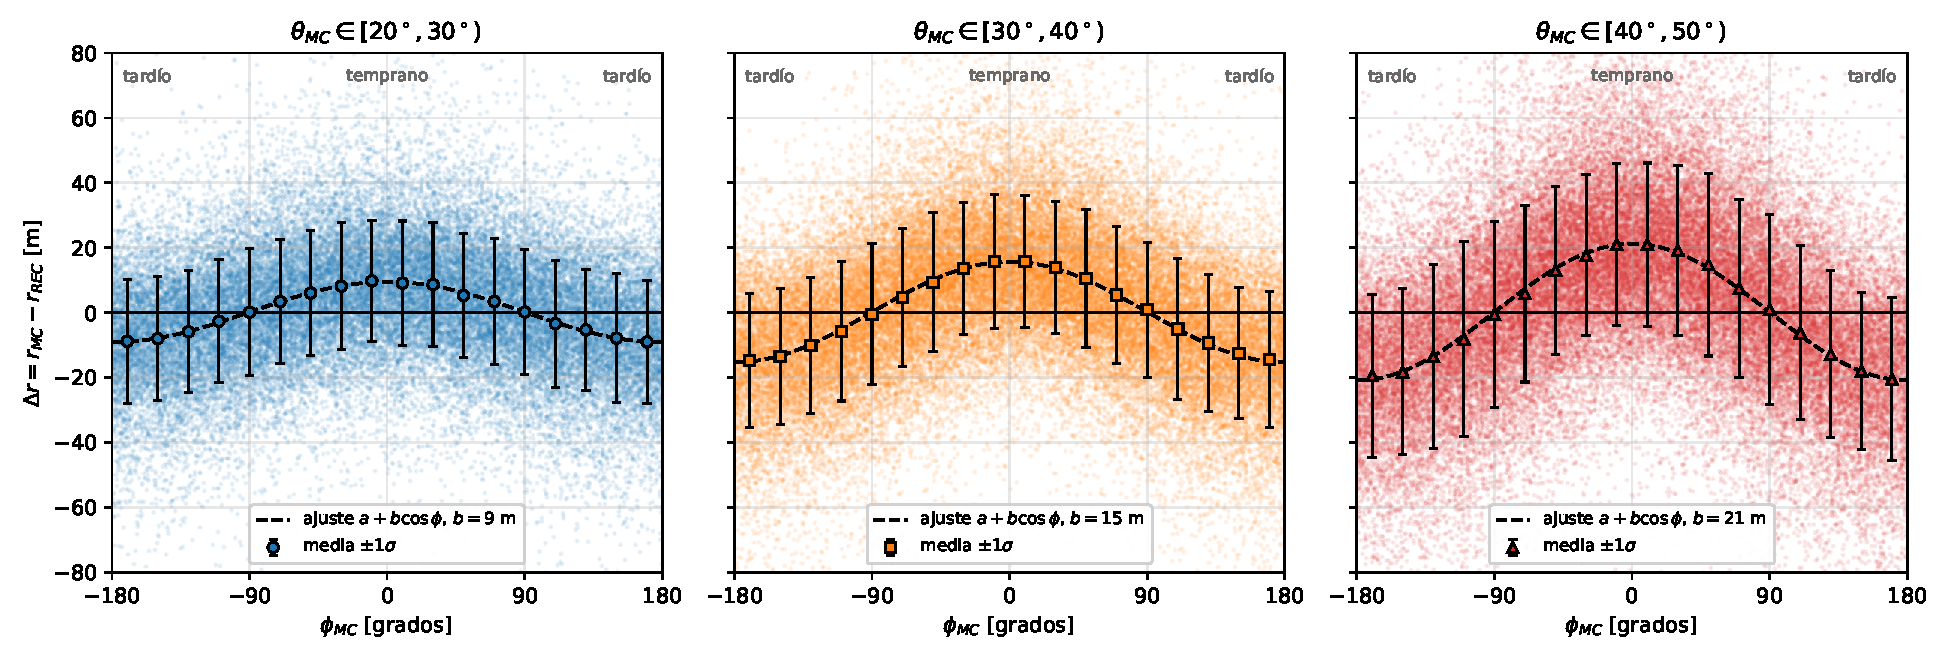
\includegraphics[width=\textwidth,height=3.2cm,keepaspectratio]{corrimiento_nucleo_azimut.pdf}

  \vspace{0.3em}
  \begin{columns}[T]
    \column{0.5\textwidth}
      \small
      \begin{itemize}
        \item El error en la posición del núcleo está en la \textbf{misma
          dirección que el eje temprano--tardío}: el núcleo reconstruido se
          corre hacia la región temprana.
        \item Por eso las estaciones tempranas quedan más cerca del núcleo REC
          ($\Delta r>0$) y las tardías, más lejos.
        \item Del ajuste $\Delta r=a+b\cos\phi$ se obtiene $b\simeq9$, $15$ y
          $21$~m: crece con $\theta$.
      \end{itemize}
    \column{0.47\textwidth}
      \small
      \begin{block}{¿Por qué?}
        La LDF de la reconstrucción es \textbf{simétrica en $\phi$}. La señal
        tiene un exceso temprano, y el único grado de libertad para
        absorberlo es acercar el núcleo a ese lado.
      \end{block}
  \end{columns}
  \fuente{Protones, \emph{Infill}.}
\end{frame}

\begin{frame}{El modelo de $\beta$}
  \badgeIF
  \vspace{-1.4em}
  \setbeamerfont{itemize/enumerate body}{size=\footnotesize}
  \begin{columns}[T]
    \column{0.58\textwidth}
      \footnotesize
      \begin{itemize}
        \item En un rango razonable de $r$, la LDF de la reconstrucción se
          puede aproximar como $\rho\propto r^{-\beta}$: \textbf{$\beta$ es su
          pendiente en log--log}, medida en las mismas simulaciones.
        \item Las estaciones se agrupan por su distancia \textbf{reconstruida},
          con el núcleo corrido \textbf{$b$} hacia la temprana. Una temprana
          está en realidad \textbf{más lejos} ($r+b$) y recibe menos muones de
          los que le corresponde; una tardía, \textbf{más cerca} ($r-b$),
          recibe más. Es una modulación en $\phi$ de \textbf{signo opuesto} a
          la física:
          \begin{equation*}
            \rho(r+b\cos\phi)\simeq\rho(r)\Big[1-\beta\,\frac{b}{r}\cos\phi\Big]
            \;\Rightarrow\;\boxed{\Delta A_1\simeq-\beta\,\frac{b}{r}}
          \end{equation*}
      \end{itemize}
    \column{0.40\textwidth}
      \scriptsize
      \centering
      \renewcommand{\arraystretch}{1.2}
      \setlength{\tabcolsep}{3pt}
      \begin{tabular}{lcccc}
        \toprule
        $\theta_{sh}$ & $b$ [m] & $\beta$ &
        \shortstack{$\Delta A_1$\\simulación} &
        \shortstack{$-\beta b/r$\\predicción}\\
        \midrule
        $20$--$30^\circ$ & $9$  & $2.9$ & $-0.051$ & $-0.051$\\
        $30$--$40^\circ$ & $15$ & $2.7$ & $-0.084$ & $-0.081$\\
        $40$--$50^\circ$ & $21$ & $2.5$ & $-0.110$ & $-0.102$\\
        \bottomrule
      \end{tabular}

      {\tiny $450\le r<600$~m, número de muones inyectado.}

      \vspace{0.3em}
      \raggedright
      \begin{itemize}
        \item \textbf{Predicción y simulación coinciden.}
        \item El corrimiento también desplaza el $\phi$ de cada estación
          (paralaje), pero sólo $\sim b/r\approx2^\circ$: usar el $\phi$
          reconstruido no cambia $A_1$.
      \end{itemize}
  \end{columns}
\end{frame}

\begin{frame}{Dos reconstrucciones, dos efectos}
  \begin{columns}[T]
    \column{0.48\textwidth}
      \begin{block}{1. Conteo de muones}
        \small
        \begin{itemize}
          \item Sobreconteo mayor del lado tardío.
          \item Anillo Denso: explica todo hasta $35^\circ$, más de la mitad
            por encima.
          \item En el \emph{Infill}: reduce $A_1$ entre un 5 y un 23\%.
        \end{itemize}
      \end{block}
    \column{0.48\textwidth}
      \begin{block}{2. Geometría reconstruida}
        \small
        \begin{itemize}
          \item Núcleo corrido hacia la región temprana.
          \item Sólo en el \emph{Infill} (en el Anillo Denso las estaciones
            están fijas).
          \item Efecto \textbf{dominante}: $\Delta A_1\simeq-\beta b/r$.
        \end{itemize}
      \end{block}
  \end{columns}
  \vspace{0.6em}
  \begin{itemize}
    \item El núcleo \textbf{no} explica el error de conteo: el número de
      muones de cada módulo no depende de dónde se reconstruye el núcleo.
    \item Mejorar el núcleo (una LDF con modulación azimutal) es tan
      importante para medir la asimetría como la respuesta del detector.
  \end{itemize}
\end{frame}

% ============================================================
\section{Datos de campo, conclusiones y trabajo futuro}
% ============================================================

\begin{frame}{Datos de campo: trabajo en curso}
  \badgeDATA
  \begin{columns}[c]
    \column{0.43\textwidth}
      \centering
      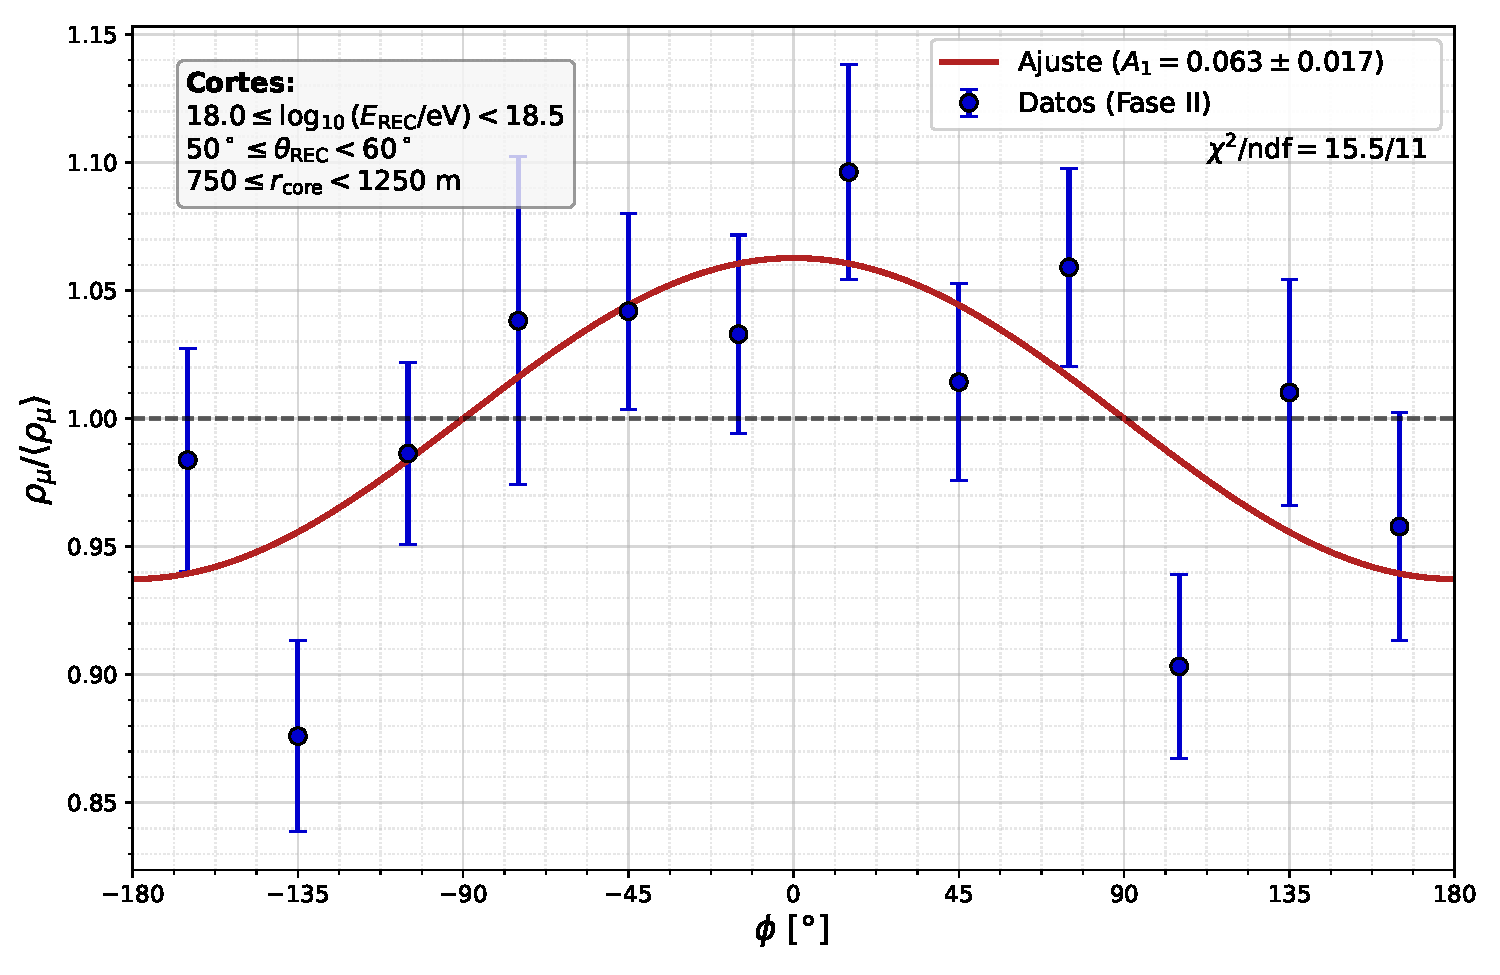
\includegraphics[width=\textwidth,height=4.2cm,keepaspectratio]{UMD_Experimental_Modulation_Corrected.pdf}
    \column{0.55\textwidth}
      \centering
      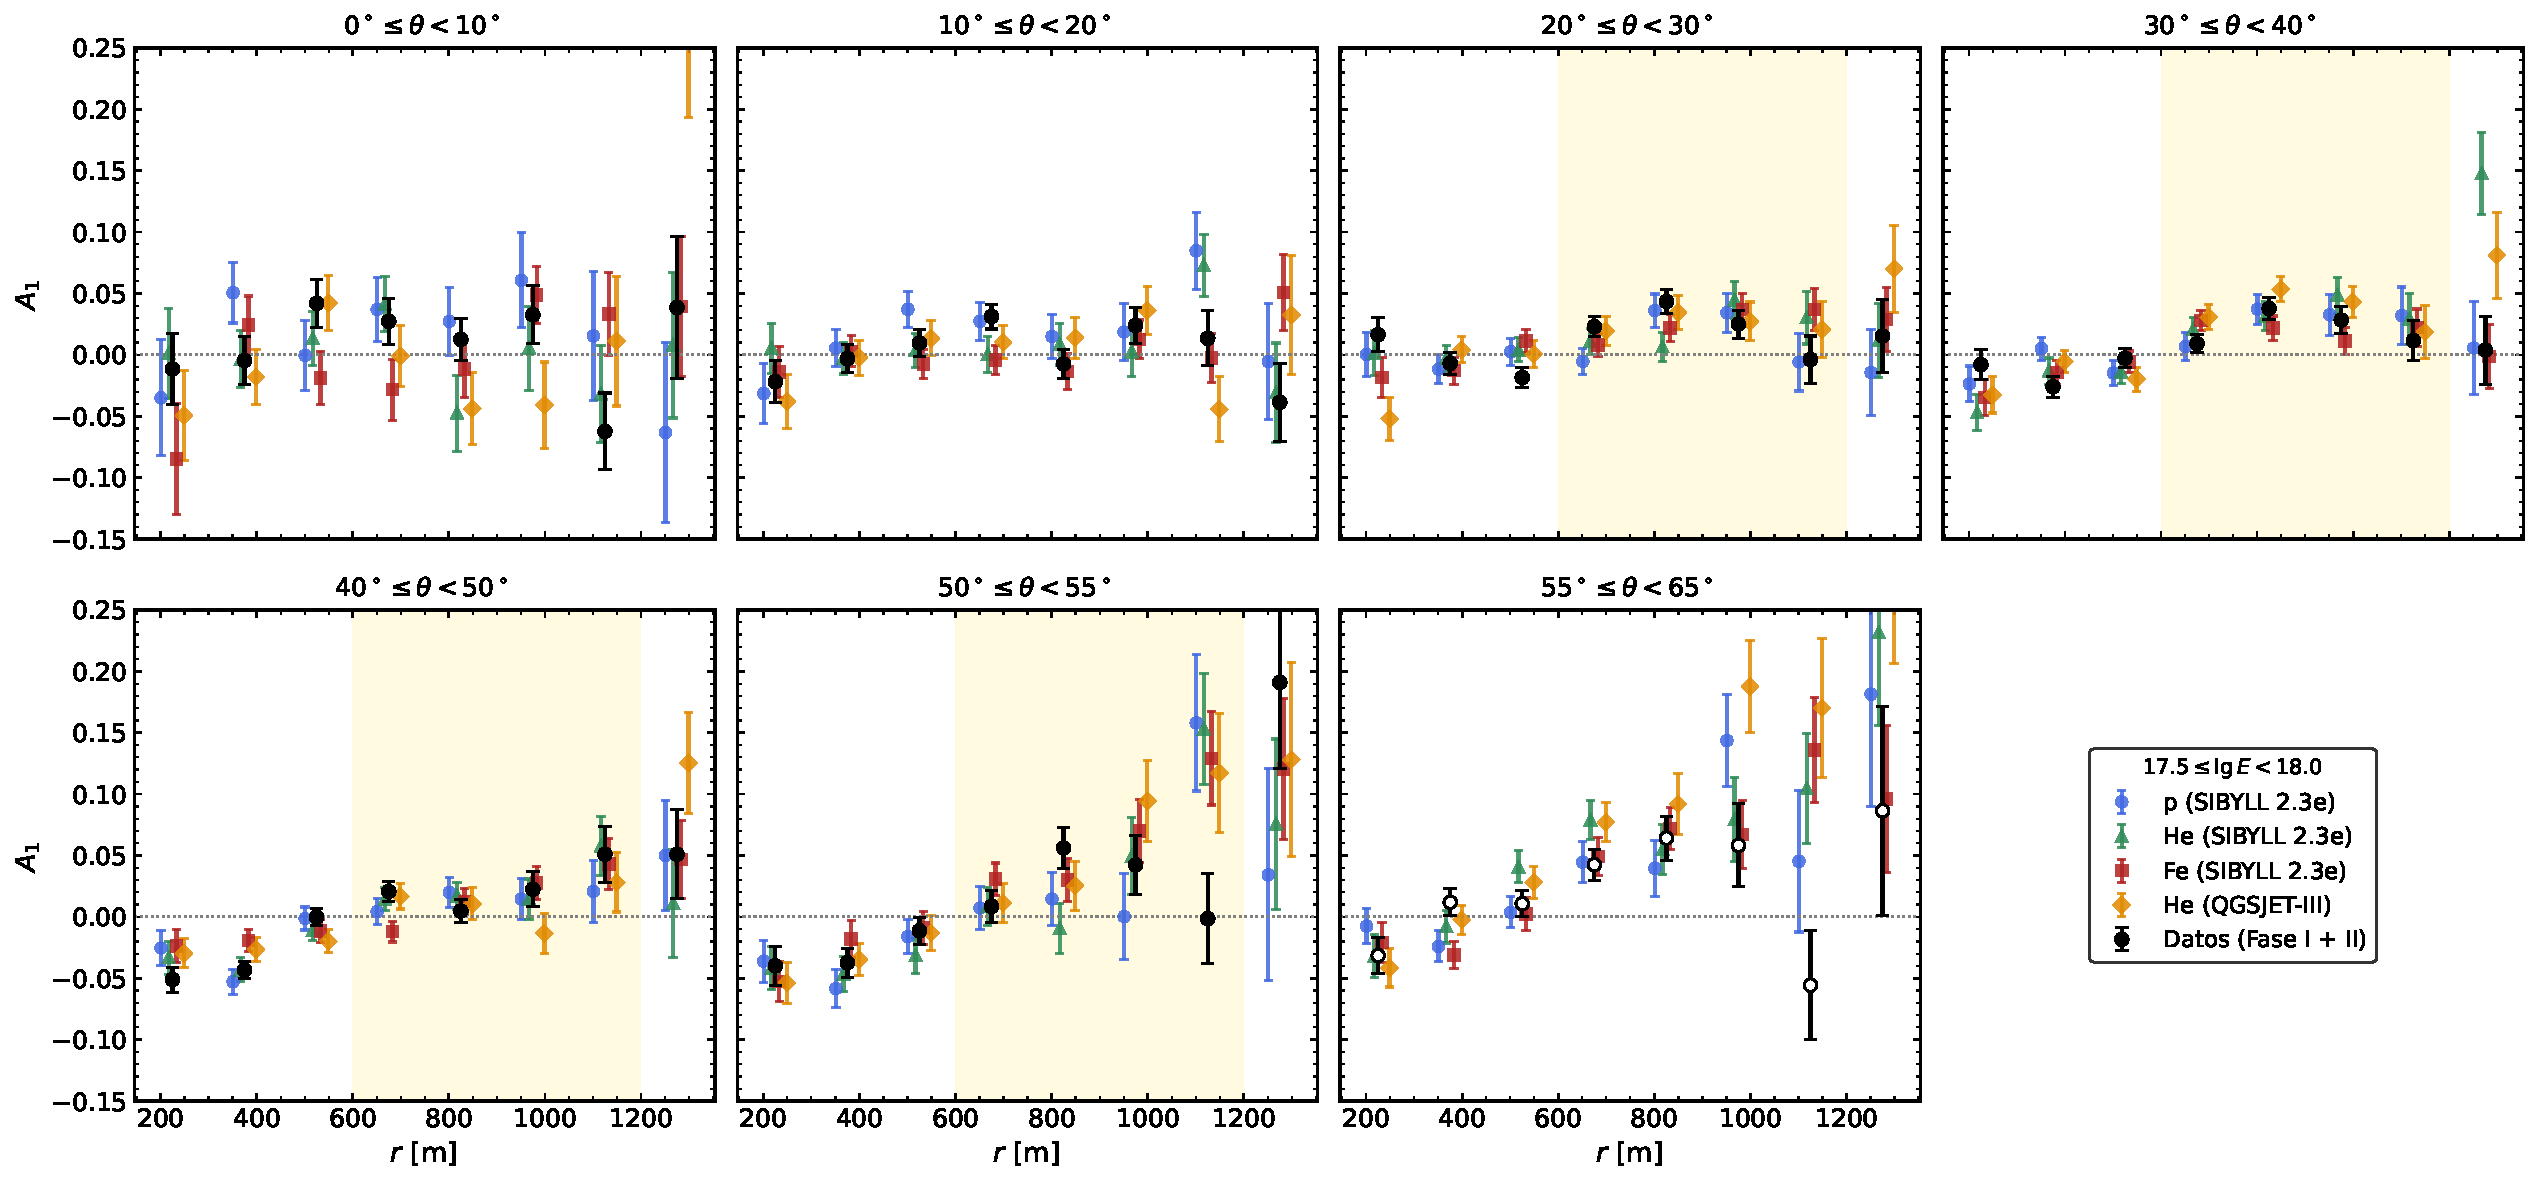
\includegraphics[width=\textwidth,height=3.5cm,keepaspectratio]{cap7_A1_vs_r_datos_vs_mc.pdf}
  \end{columns}
  \small
  \begin{itemize}
    \item UMD \emph{Infill}, producción \texttt{v4r2}, Fase~I + Fase~II, 6T5, $\lg(E/\text{eV})\ge17.5$.
    \item Fase~II, $18.0\le\lg E<18.5$, $50^\circ\le\theta<60^\circ$,
      $750\le r<1250$~m: \alert{$A_1=0.063\pm0.017$}, máximo en la región
      temprana.
    \item $A_1(r)$: los datos siguen a las simulaciones reconstruidas, incluido
      el $A_1<0$ cerca del núcleo en lluvias inclinadas (núcleo corrido).
  \end{itemize}
\end{frame}

\begin{frame}{Conclusiones}
  \setbeamerfont{itemize/enumerate body}{size=\footnotesize}
  \small
  \begin{enumerate}
    \item \textbf{Asimetría en el UMD.} Positiva y creciente con $r$ y $\theta$,
      como predice el modelo. El SD se aparta por un \textbf{sesgo de
      selección}: sobre todas las estaciones, sus muones vuelven a ser
      positivos ($+0.069\pm0.016$ frente a $-0.124\pm0.019$).
    \item \textbf{Sensibilidad a la masa.} En el Anillo Denso,
      $A_1^{\text{p}}>A_1^{\text{Fe}}$ con $S\sim2.5$ a $40^\circ$--$55^\circ$,
      y $A_1$ crece con $E$: consistente con un $X_{\max}$ más profundo. Falta
      medir la variabilidad entre submuestras para hablar de discriminación.
    \item \textbf{Modelo analítico.} Cuatro mecanismos en un modelo de juguete
      que recupera la expresión de Armbruster. Sus predicciones ($A_1>0$,
      creciente con $r$ y $\theta$, UMD por encima del SD) se
      \textbf{confirmaron en las simulaciones}: parece una descripción
      fenomenológica bastante completa del signo y de las tendencias.
  \end{enumerate}
  \begin{block}{Además}
    La reconstrucción reduce $A_1$ por dos vías: el conteo de muones (sesgo
    direccional) y el \textbf{corrimiento del núcleo},
    $\Delta A_1\simeq-\beta b/r$. Primera observación de la modulación en
    datos del UMD.
  \end{block}
\end{frame}

\begin{frame}{Trabajo futuro}
  \begin{itemize}
    \item \textbf{Datos de campo}: incertezas sistemáticas, comparación
      cuantitativa con simulaciones en todo el espacio de fases, simulaciones
      por encima de $10^{18}$~eV.
    \item \textbf{Masa y energía en el \emph{Infill}}, y variabilidad de $A_1$
      entre submuestras: ¿con cuántos eventos se distinguen dos composiciones?
    \item \textbf{Remanente} de la degradación por encima de $35^\circ$.
    \item \textbf{Selección del SD}: separar disparo, lectura y reconstrucción.
    \item \textbf{Núcleo}: una LDF con modulación azimutal, al menos en los
      eventos de mayor multiplicidad.
    \item Un \textbf{modelo cinemático} de producción y transporte (CORSIKA +
      Cazón) que prediga amplitudes, no sólo signos.
    \item El efecto del \textbf{déficit de muones} de los modelos sobre $A_1$.
  \end{itemize}
\end{frame}

\begin{frame}[plain]
  \begin{tikzpicture}[remember picture, overlay]
    % Imagen a pantalla completa (más ancha que la slide: se recorta a los costados).
    \node[anchor=center, inner sep=0pt] at (current page.center)
      {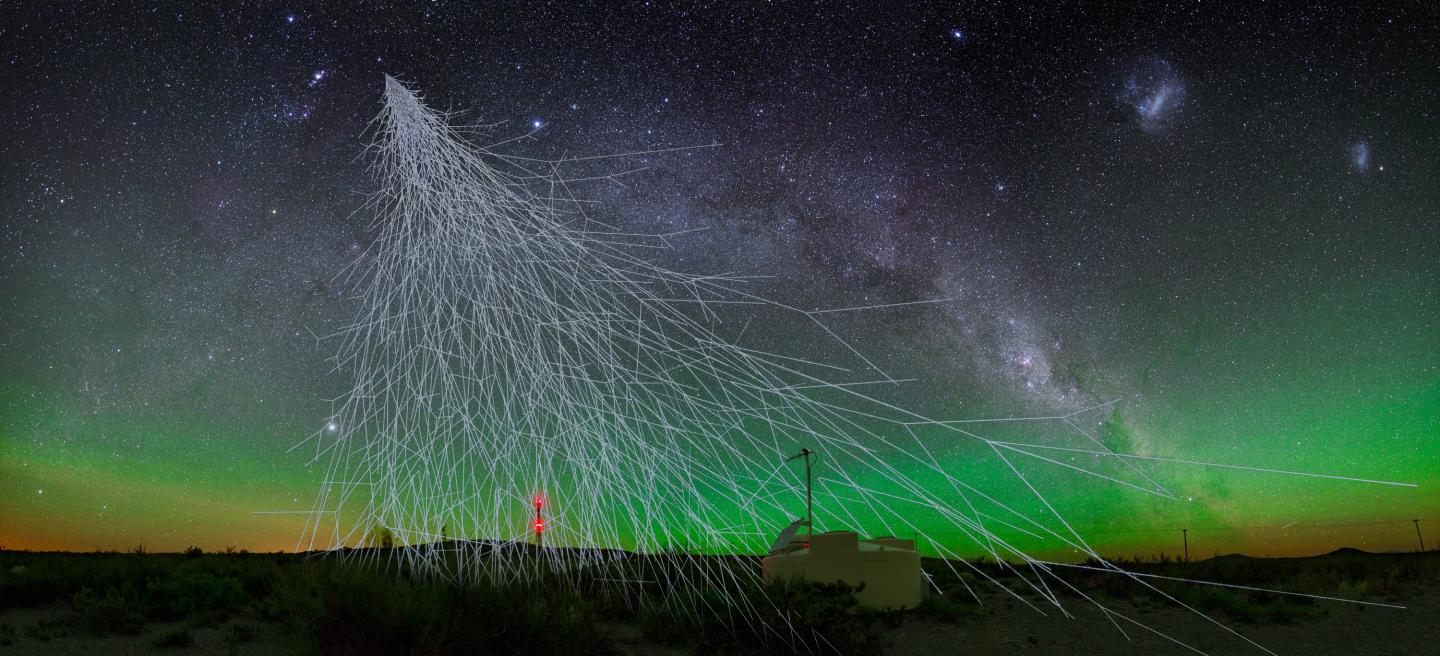
\includegraphics[height=\paperheight]{auger_cr.jpg}};
    % Texto arriba a la derecha, sobre el cielo oscuro, con una sombra suave.
    \node[anchor=north east, xshift=-0.86cm, yshift=-0.49cm, text=black, opacity=0.6,
      font=\fontsize{34}{38}\selectfont\bfseries] at (current page.north east) {¡Gracias!};
    \node[anchor=north east, xshift=-0.9cm, yshift=-0.45cm, text=white,
      font=\fontsize{34}{38}\selectfont\bfseries] at (current page.north east) {¡Gracias!};
    \node[anchor=north east, xshift=-0.91cm, yshift=-1.79cm, text=black, opacity=0.6,
      font=\LARGE\bfseries] at (current page.north east) {¿Preguntas?};
    \node[anchor=north east, xshift=-0.95cm, yshift=-1.75cm, text=itedaOrange,
      font=\LARGE\bfseries] at (current page.north east) {¿Preguntas?};
    \node[anchor=south east, xshift=-0.15cm, yshift=0.1cm, text=white, opacity=0.8,
      font=\tiny] at (current page.south east)
      {Imagen: A.~Chantelauze, S.~Staffi, L.~Bret (Observatorio Pierre Auger)};
  \end{tikzpicture}
\end{frame}

% ============================================================
\appendix
% ============================================================

\begin{frame}{Backup: incertezas de $A_1$ y significado de $S$}
  \small
  \begin{itemize}
    \item $\sigma_{A_1}$ sale del ajuste, con el error estándar de la media en
      cada bin de $\phi$ como incerteza.
    \item Ese error trata como independientes a las estaciones de una misma
      lluvia, y en el Anillo Denso cada lluvia de CORSIKA se reconstruye 5
      veces con el núcleo desplazado.
    \item $\chi^2_\nu\approx1$ no lo valida del todo: las fluctuaciones de
      normalización de cada lluvia se cancelan en la forma.
    \item En el estudio de selección del SD (Cap.~6) los errores se
      estimaron con \emph{bootstrap} sobre lluvias. Para el Anillo Denso,
      ese \emph{bootstrap} queda pendiente.
    \item $S$ mide la diferencia de \textbf{medias} con la estadística
      disponible ($\propto\sqrt{N}$); no es un factor de mérito evento a
      evento.
  \end{itemize}
\end{frame}

\begin{frame}{Backup: grillas con geometría MC y REC}
  \badgeIF
  \begin{columns}[T]
    \column{0.5\textwidth}
      \centering\footnotesize Geometría Monte Carlo, $30^\circ$--$40^\circ$\\
      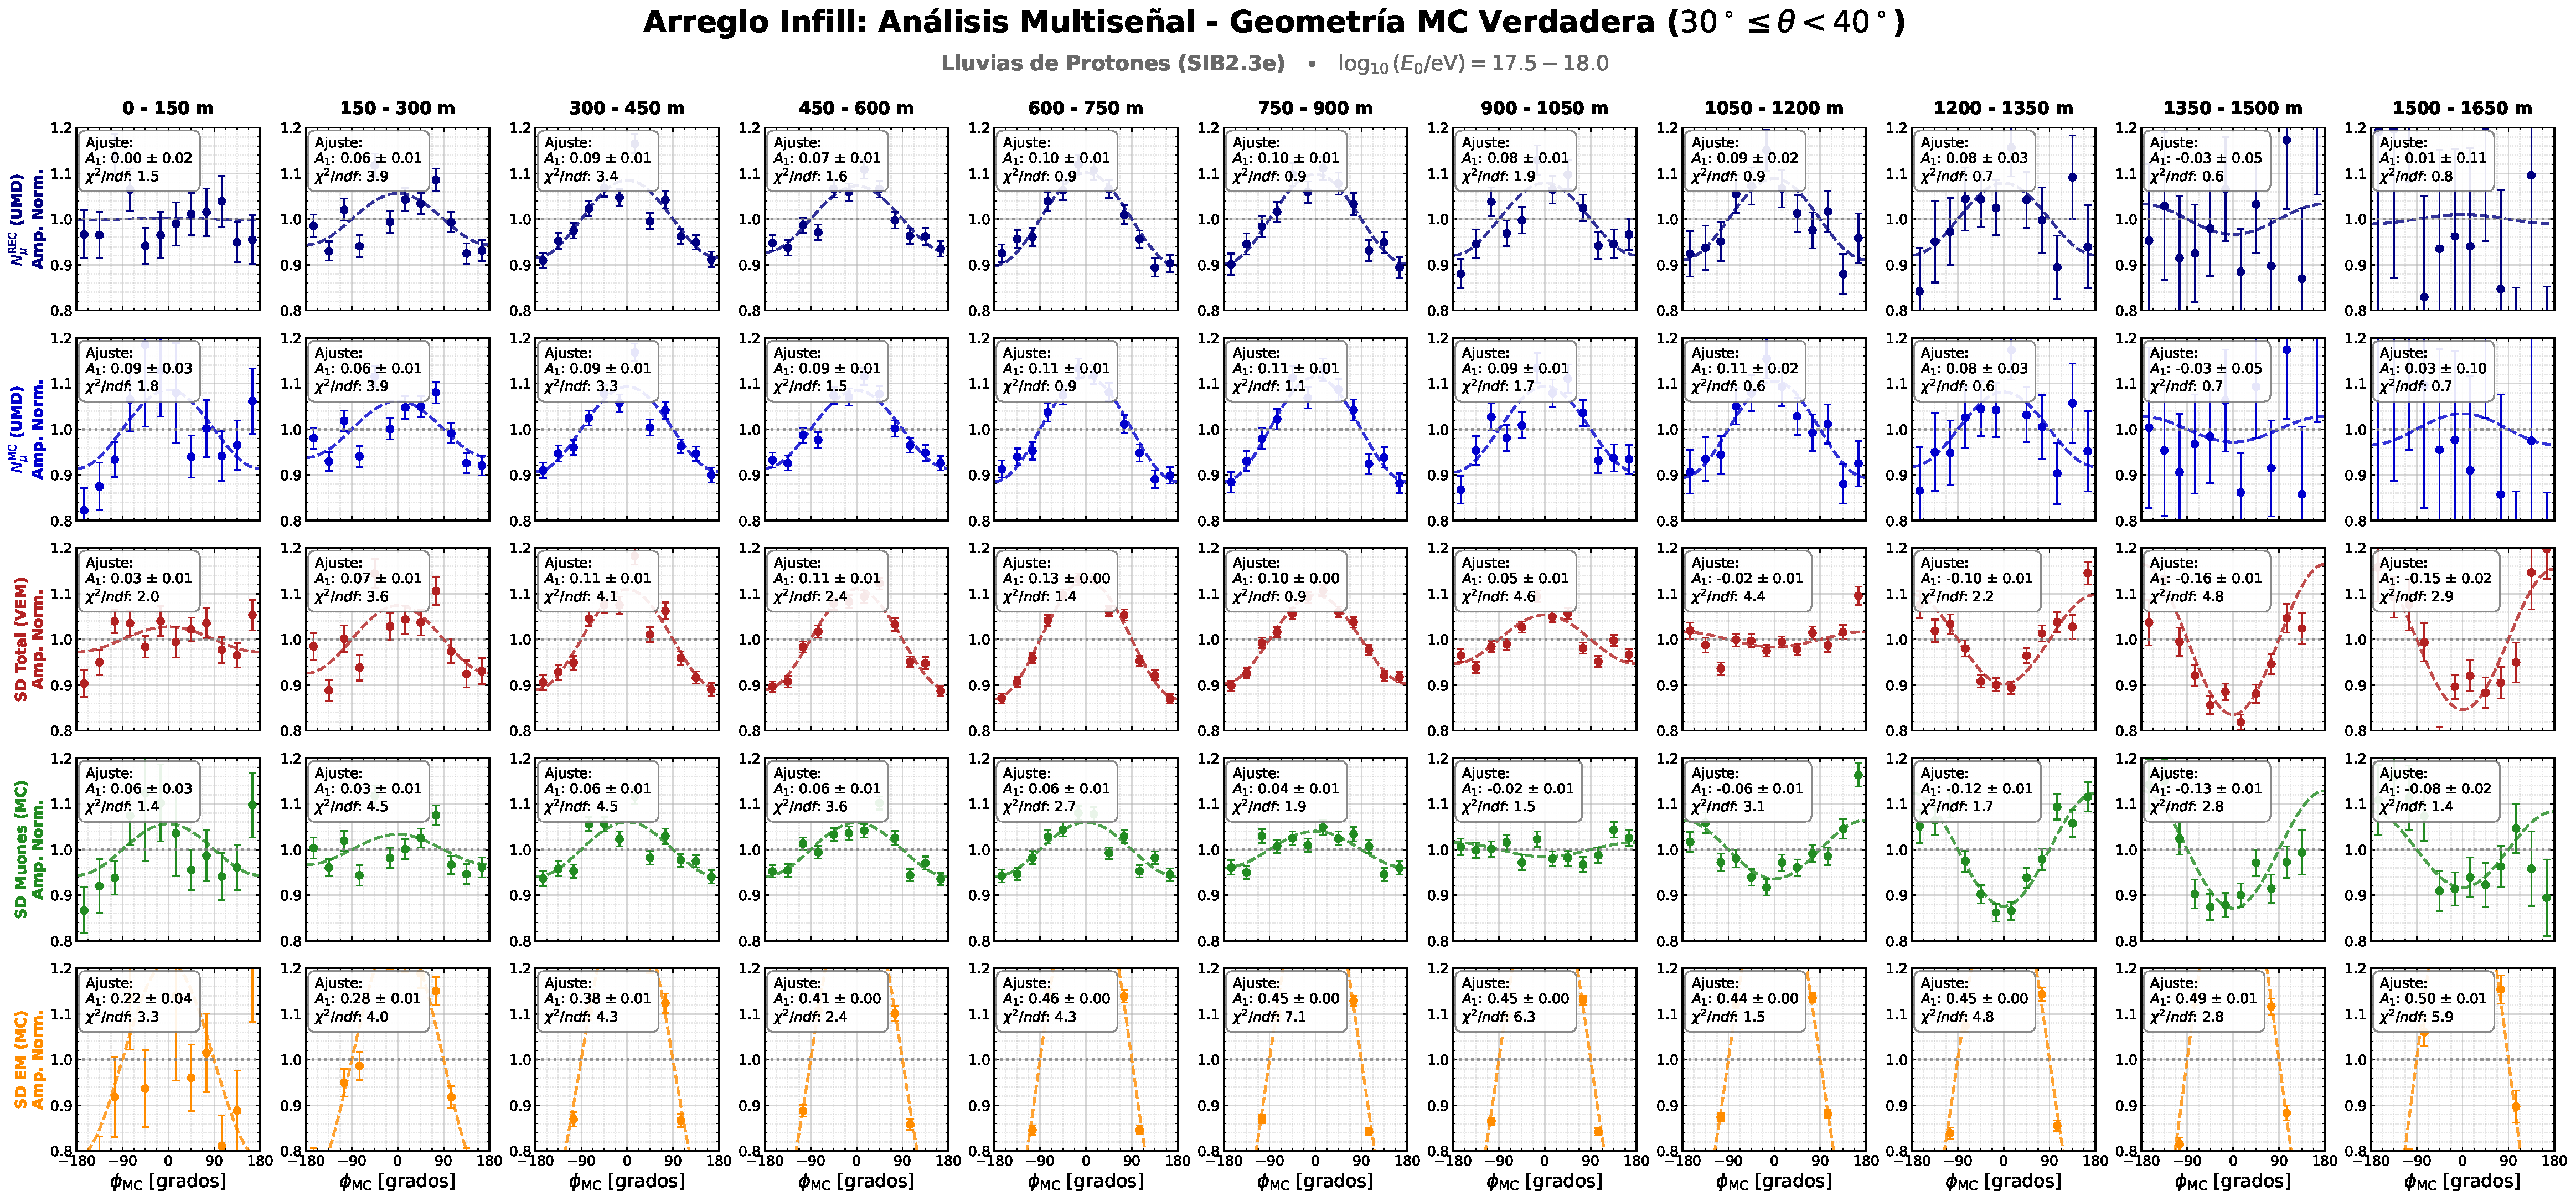
\includegraphics[width=\textwidth]{Anexo_Grilla_MC_30_40.pdf}
    \column{0.5\textwidth}
      \centering\footnotesize Geometría reconstruida, $30^\circ$--$40^\circ$\\
      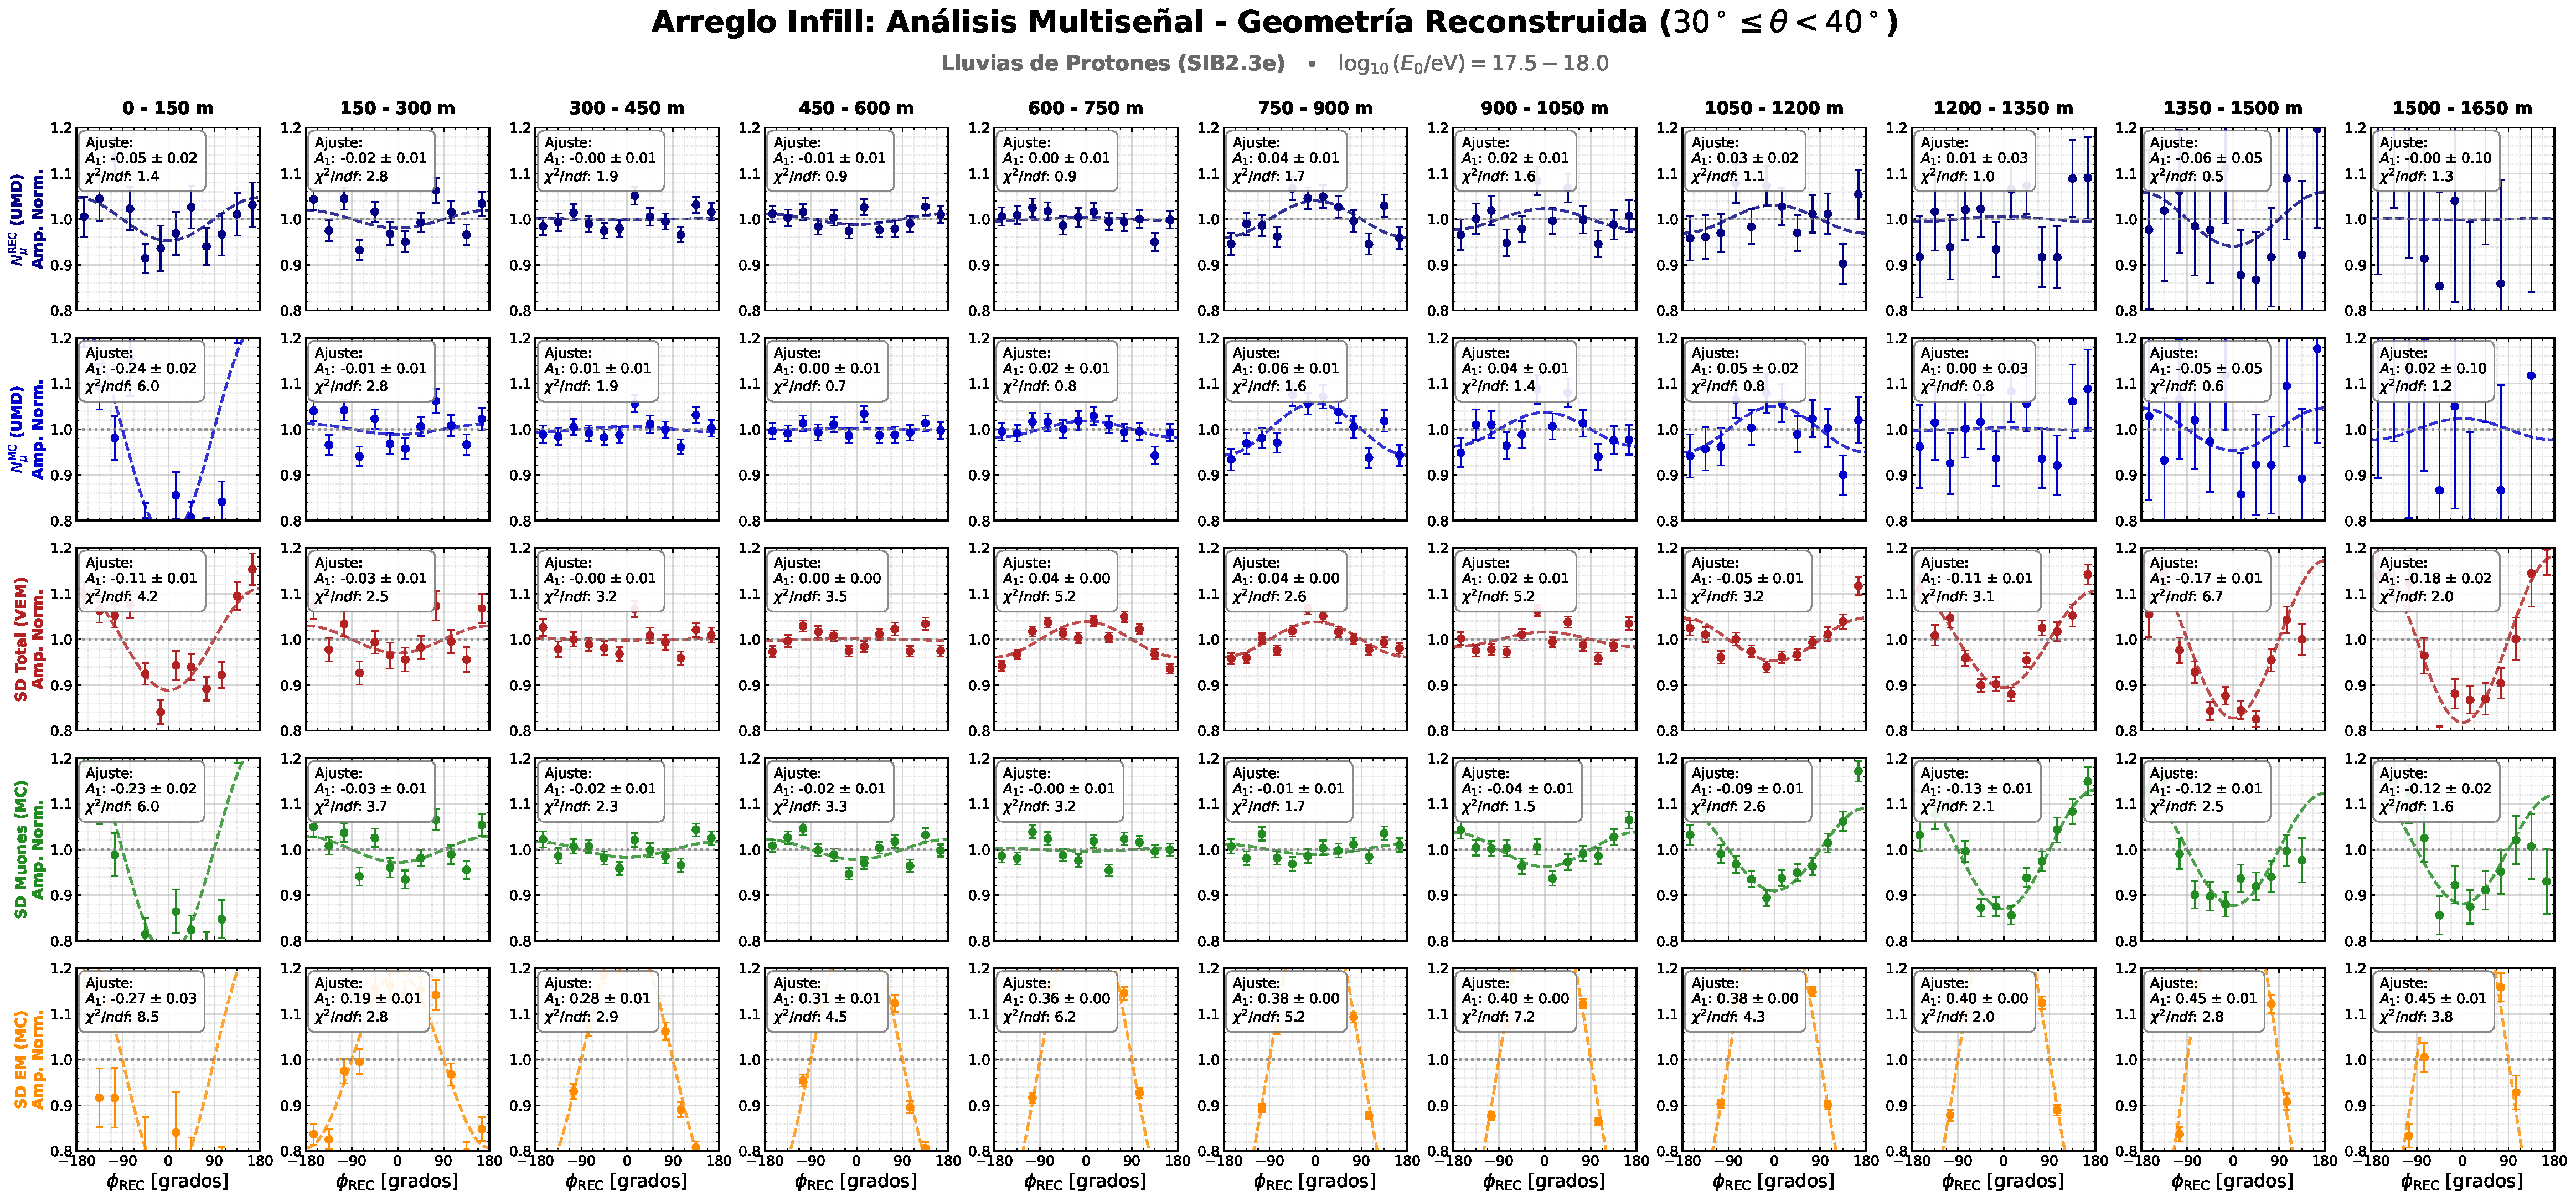
\includegraphics[width=\textwidth]{Anexo_Grilla_REC_30_40.pdf}
  \end{columns}
  \small
  \begin{itemize}
    \item Mismas lluvias y mismos módulos: con la geometría reconstruida la
      modulación se reduce en casi todos los bines radiales. A
      $40^\circ$--$50^\circ$, $A_1\lesssim0.05$ entre 600 y 1050~m frente a
      $\approx0.11$ con geometría MC.
  \end{itemize}
\end{frame}

\begin{frame}{Backup: conteo REC vs.\ MC (geometría MC)}
  \badgeIF
  \begin{columns}[c]
    \column{0.6\textwidth}
      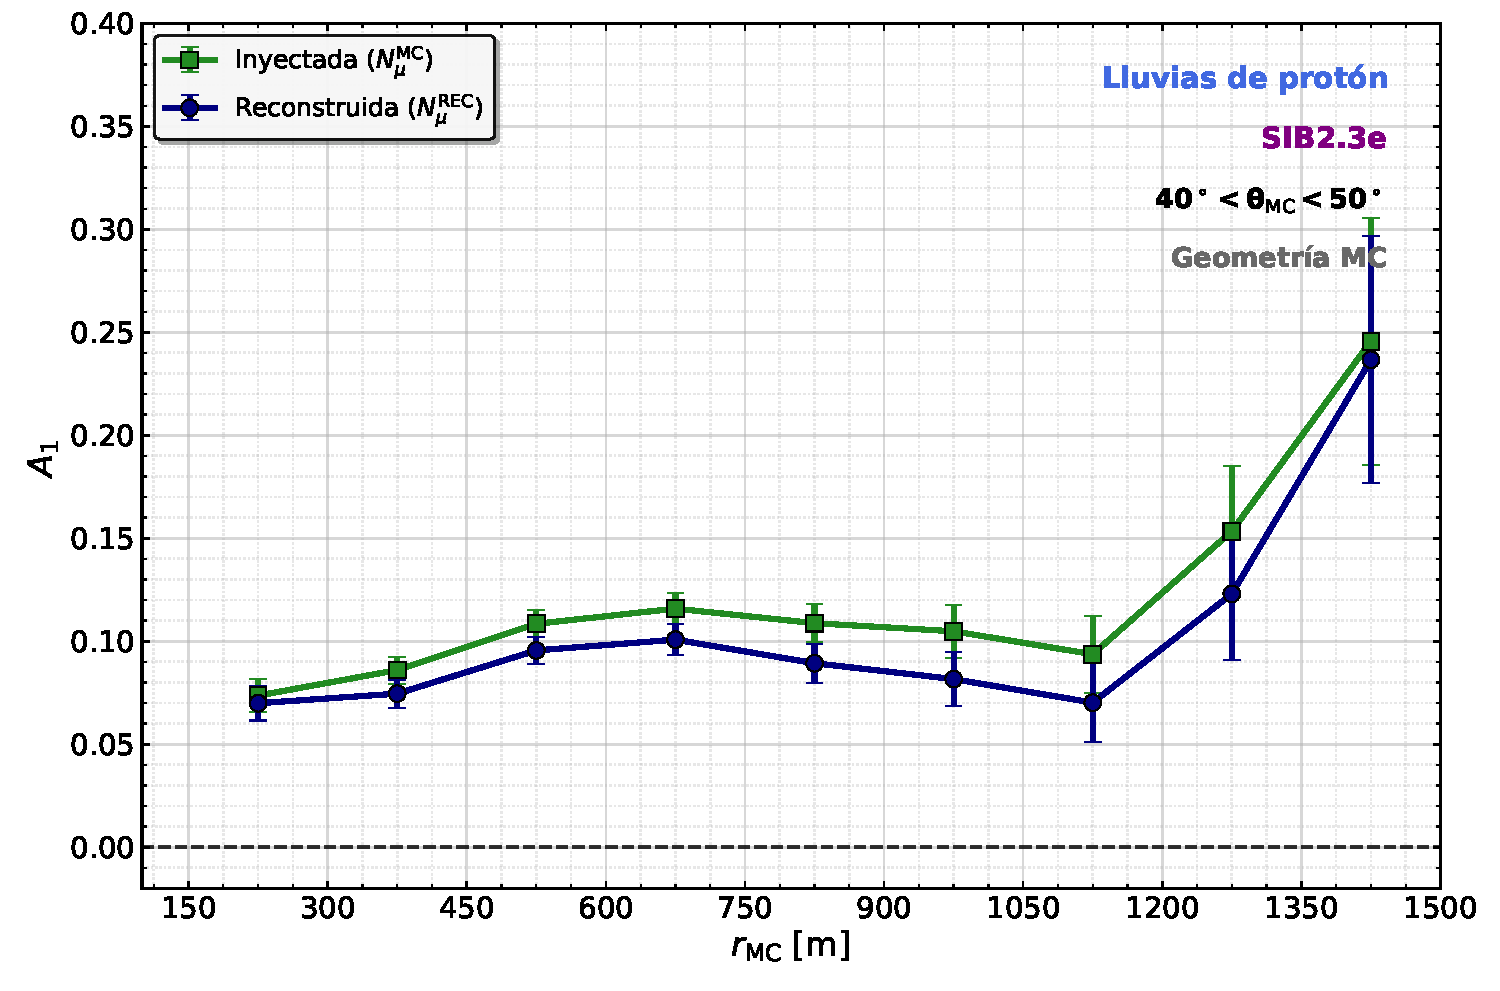
\includegraphics[width=\textwidth]{UMD_Asymmetry_MC_vs_REC.pdf}
    \column{0.37\textwidth}
      \small
      \begin{itemize}
        \item $40^\circ$--$50^\circ$, núcleo y dirección MC.
        \item El conteo reconstruido reduce $A_1$ un 5--23\% sin cambiar su
          forma.
      \end{itemize}
  \end{columns}
\end{frame}

\begin{frame}{Backup: datos de campo --- región de referencia y fases}
  \badgeDATA
  \footnotesize
  Región de referencia (franja sombreada en la slide de datos de campo): $600\le r<1200$~m, $20^\circ\le\theta<55^\circ$,
  $17.5\le\lg E<18.0$. Media de $A_1$ sobre las 16 celdas (salida de
  \texttt{Analisis\_Asimetria\_DatosCampo\_Cap7.py}; \textbf{no figura en la tesis}):
  \begin{center}
    \renewcommand{\arraystretch}{1.1}
    \begin{tabular}{lc@{\hspace{2em}}lc}
      \toprule
      Datos (Fase I + II) & $0.023\pm0.003$ & SIBYLL p & $0.017\pm0.004$\\
      Fase I & $0.010\pm0.008$ & SIBYLL He & $0.022\pm0.004$\\
      Fase II & $0.023\pm0.003$ & SIBYLL Fe & $0.019\pm0.003$\\
      & & QGSJET He & $0.028\pm0.004$\\
      \bottomrule
    \end{tabular}
  \end{center}
  \begin{itemize}
    \item Datos compatibles con las simulaciones; \textbf{sin separación
      p/Fe} con geometría REC a esta estadística.
    \item Fase I vs.\ Fase II celda a celda: $\chi^2=103/53$; Fase I tiene
      mucha menos estadística. Pendiente de entender.
    \item Exposición en $\phi$ no uniforme: su término en $\cos\phi$ es
      similar en datos y MC (0.22 y 0.24 a 900--1200~m).
  \end{itemize}
\end{frame}

\begin{frame}{Backup: muestra de datos de campo}
  \badgeDATA
  \centering
  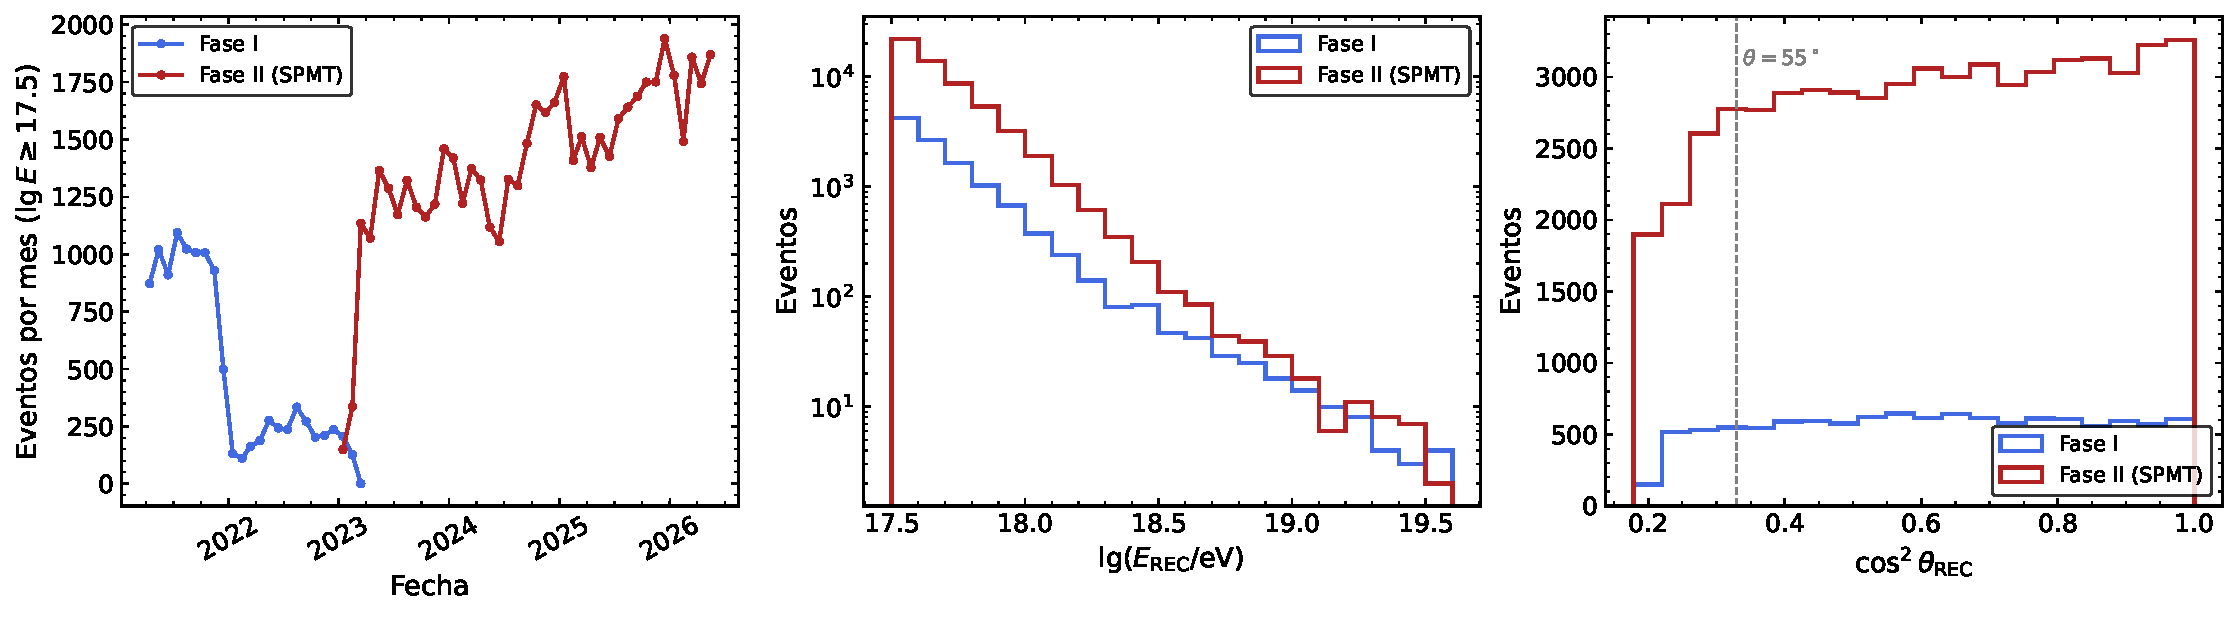
\includegraphics[width=\textwidth]{cap7_dataset.pdf}
  \small
  \begin{itemize}
    \item Fase~I (abr 2021 -- abr 2023) y Fase~II SPMT (feb 2022 -- may 2026),
      sin el período de puesta en marcha de 2022. Eventos disjuntos entre fases.
  \end{itemize}
\end{frame}

\begin{frame}{Backup: reconstrucción de energía y dirección}
  \badgeMC
  \begin{columns}[T]
    \column{0.33\textwidth}
      \centering
      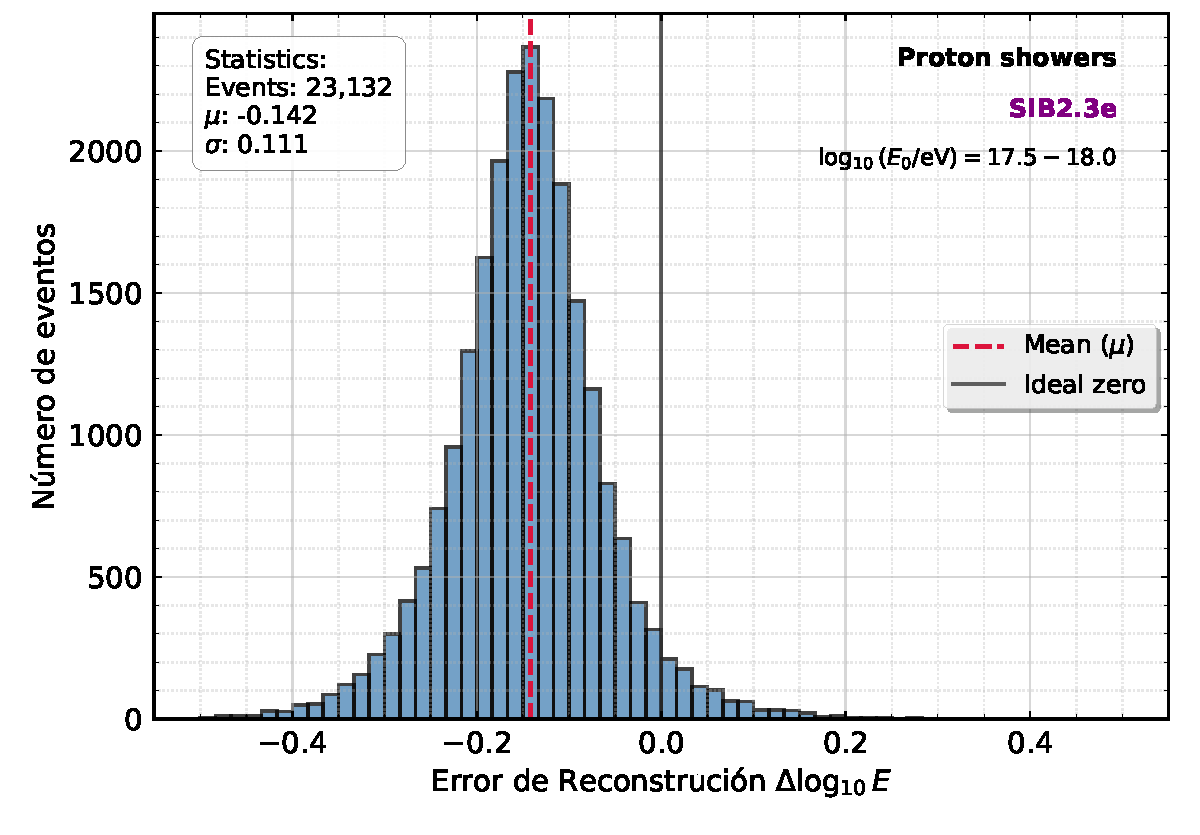
\includegraphics[width=\textwidth]{energy_bias.pdf}
    \column{0.33\textwidth}
      \centering
      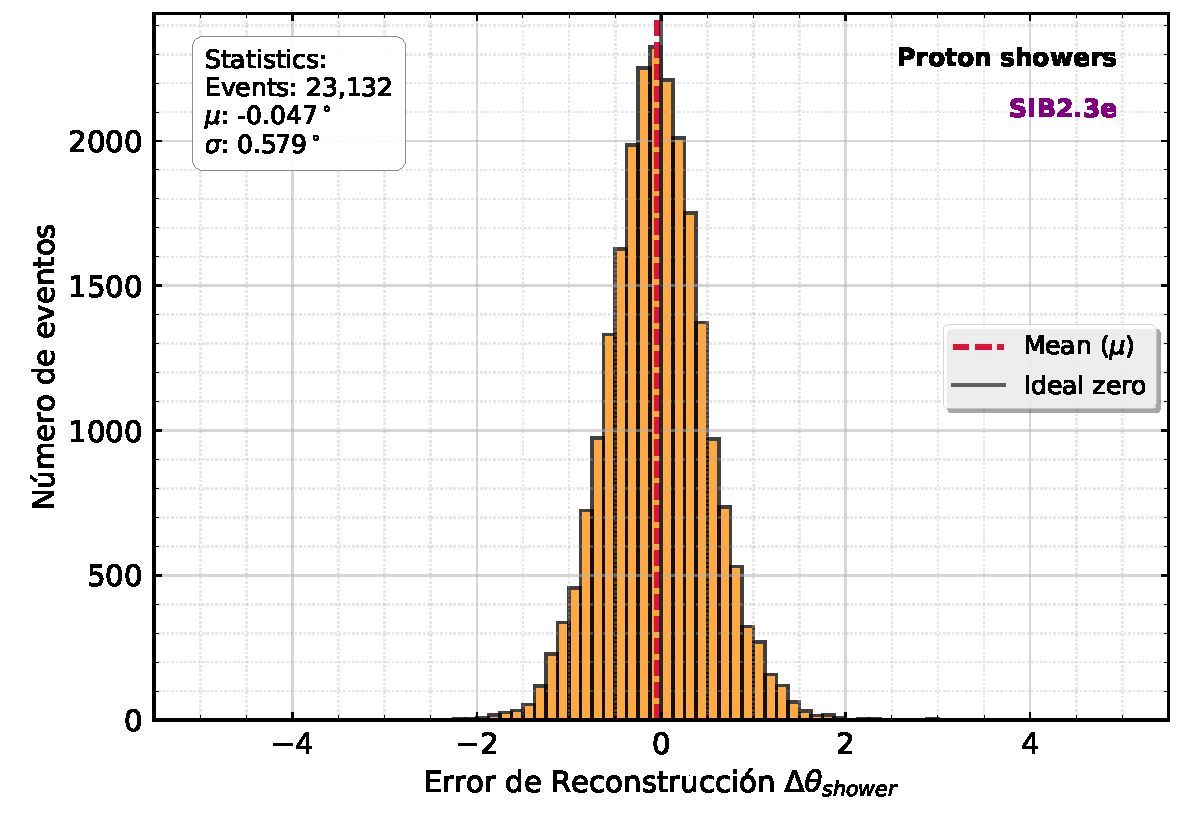
\includegraphics[width=\textwidth]{theta_bias.pdf}
    \column{0.33\textwidth}
      \centering
      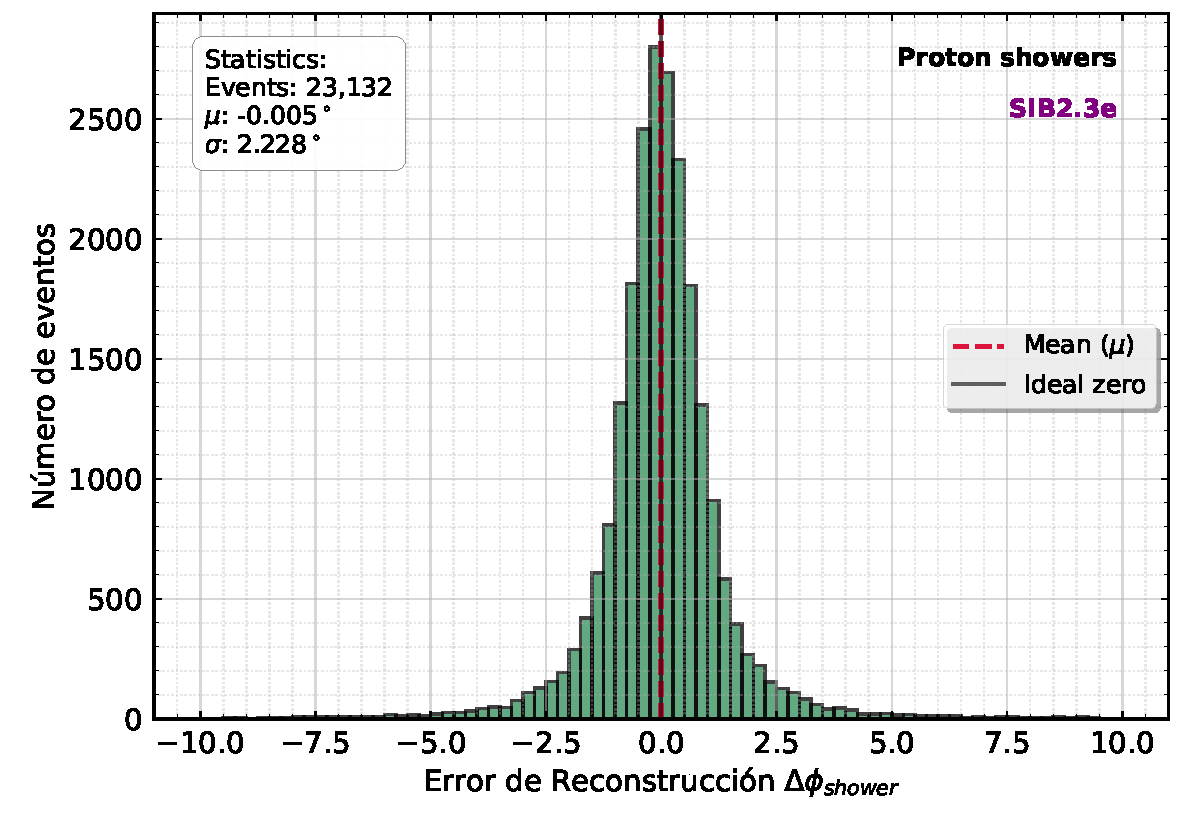
\includegraphics[width=\textwidth]{phi_bias.pdf}
  \end{columns}
  \small
  \begin{itemize}
    \item Energía: $\mu\approx-0.142$, $\sigma\approx0.111$ en
      $\Delta\log_{10}E$ ($\approx28\%$ de subestimación, déficit de muones).
    \item $\theta$: sesgo $-0.05^\circ$, $\sigma=0.58^\circ$. $\phi$: sesgo
      $-0.005^\circ$, $\sigma=2.2^\circ$.
  \end{itemize}
\end{frame}

\begin{frame}{Backup: ajuste del SD en el Anillo Denso}
  \badgeAD
  \begin{columns}[c]
    \column{0.6\textwidth}
      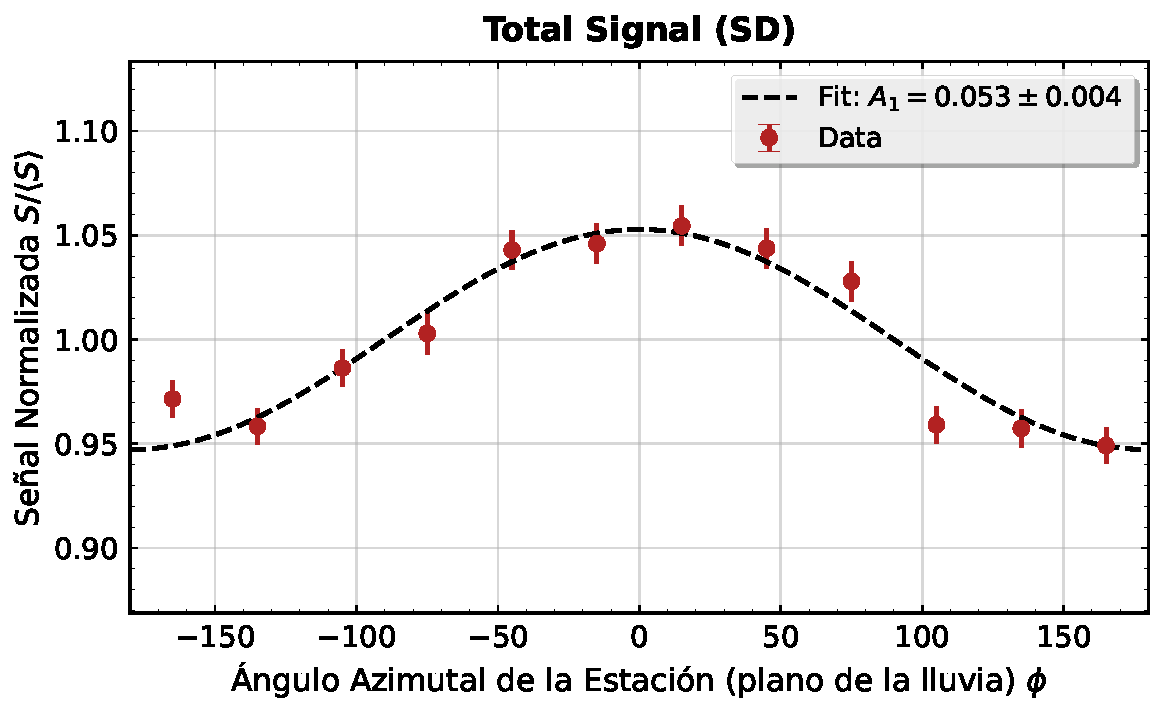
\includegraphics[width=\textwidth]{Ajuste_SD_Total_Bin9.pdf}
    \column{0.37\textwidth}
      \small
      \begin{itemize}
        \item Errores imperceptibles por la gran estadística EM.
        \item El armónico describe la tendencia; el $\chi^2_\nu$ alto refleja
          residuos de orden superior.
      \end{itemize}
  \end{columns}
\end{frame}

\end{document}
